\documentclass[12pt,a4paper]{article}
\usepackage[utf8]{inputenc}
\usepackage[portuguese]{babel}
\usepackage{geometry}
\usepackage{graphicx}
\usepackage[unicode=false]{hyperref}
\usepackage{longtable}
\usepackage{array}
\usepackage{booktabs}
\usepackage{enumitem}
\usepackage{float}
\usepackage{tikz}
\usepackage{microtype}

\geometry{
    left=3cm,
    right=2cm,
    top=3cm,
    bottom=2cm
}

\hypersetup{
    colorlinks=true,
    linkcolor=black,
    filecolor=magenta,      
    urlcolor=cyan,
    citecolor=black,
    hypertexnames=false
}

% Aumenta tolerância a quebras de linha longas e reduz overfull/underfull boxes
\emergencystretch=1em
\sloppy

\begin{document}

\begin{titlepage}
    \centering
    \vspace*{2cm}
    
    \huge
    \textbf{Laboratório de Engenharia de Software}
    
    \vspace{1.5cm}
    \Large
    \textbf{Projeto: Plataforma de Acessibilidade Urbana com IA}
    
    \vfill
    
    \large
    \textbf{São Paulo}\\
    \textbf{2025}
    
    \vspace{2cm}
\end{titlepage}

\tableofcontents
\newpage

\section{Introdução}
\label{sec:introducao}

O Projeto em questão é uma aplicação Web que tem como ponto central a sistematização do processo de relato, monitoramento e divulgação das falhas de problemas de acessibilidade, na rede de transporte público de grandes centros urbanos. A proposta é inspirada pelo Objetivo de Desenvolvimento Sustentável (ODS) de número 11, sobre Cidades e Comunidades Sustentáveis, da Organização das Nações Unidas (ONU).

A plataforma proposta utiliza tecnologias acessíveis para criar um mapa colaborativo de barreiras de acessibilidade urbana na rede pública de transporte, transformando dados enviados por cidadãos em informações estruturadas e acionáveis para gestão pública.

\section{Definição da Demanda}
\label{sec:definicao-demanda}

\subsection{Problema/Oportunidade Percebida}
\label{subsec:problema-oportunidade}

As cidades brasileiras enfrentam graves deficiências em acessibilidade urbana, impactando diretamente a qualidade de vida de pessoas com mobilidade reduzida, idosos, usuários de cadeiras de rodas, pessoas com deficiência visual e famílias com carrinhos de bebê. Os principais problemas identificados incluem:

\begin{itemize}
    \item \textbf{Falta de dados estruturados}: inexistência de base centralizada e atualizada sobre barreiras de acessibilidade
    \item \textbf{Informações fragmentadas}: relatos dispersos em redes sociais e canais isolados sem sistematização
    \item \textbf{Ausência de priorização técnica}: gestores públicos tomam decisões sem dados concretos sobre impacto e urgência
    \item \textbf{Invisibilidade do problema}: barreiras não documentadas perpetuam a exclusão social
    \item \textbf{Alto custo de mapeamento manual}: levantamentos tradicionais demandam recursos humanos e tempo excessivos
    \item \textbf{Baixa transparência social}: ausência de acesso público e acompanhamento das ações reduz a confiança e a participação cidadã
\end{itemize}

\subsection{Razão/Justificativa da Demanda}
\label{subsec:razao-justificativa}

A demanda por uma solução tecnológica de mapeamento de acessibilidade urbana se justifica pelos seguintes fatores:

\begin{itemize}
    \item \textbf{Impacto social}: 17,2 milhões de brasileiros com dificuldade de locomoção (IBGE 2019) enfrentam perda de autonomia e dignidade
    \item \textbf{Conformidade legal}: Necessidade de cumprimento da Lei Brasileira de Inclusão (Lei 13.146/2015)
    \item \textbf{Eficiência na gestão pública}: Má alocação de recursos públicos em intervenções não prioritárias devido à falta de dados
    \item \textbf{Inclusão social}: Barreiras arquitetônicas perpetuam a exclusão de uma parcela significativa da população
    \item \textbf{Sustentabilidade urbana}: Alinhamento com os Objetivos de Desenvolvimento Sustentável da ONU
\end{itemize}

\subsection{Descrição do Produto de Software}
\label{subsec:descricao-produto}

A solução proposta é uma plataforma open-source que utiliza tecnologias acessíveis para criar um mapa colaborativo e inteligente de barreiras de acessibilidade urbana. Os componentes principais incluem:

Principais componentes:
\begin{itemize}
    \item \textbf{Sistema de Coleta Colaborativa:} cidadãos reportam problemas com fotos e geolocalização.
    \item \textbf{Plataforma de Dados Abertos:} disponibilização pública dos dados.
    \item \textbf{Mapa Interativo:} visualização em tempo real das barreiras.
    \item \textbf{Painel de Gestão:} dashboard para gestores públicos e sociedade civil acompanharem indicadores.
\end{itemize}

\subsection{Clientes, Usuários e Demais Grupos de Interesse}
\label{subsec:clientes-usuarios}

\textbf{Usuários Primários:}
\begin{itemize}
    \item Pessoas com deficiência física, visual ou mobilidade reduzida
    \item Idosos
    \item Famílias com crianças pequenas (carrinhos de bebê)
    \item Cidadãos engajados em causas de acessibilidade
\end{itemize}

\textbf{Clientes/Beneficiários:}
\begin{itemize}
    \item Prefeituras e órgãos de gestão urbana
    \item Secretarias de mobilidade e acessibilidade
    \item Organizações da sociedade civil
    \item Pesquisadores e acadêmicos
\end{itemize}

\textbf{Grupos de Interesse:}
\begin{itemize}
    \item Conselhos municipais de pessoas com deficiência
    \item Empresas de tecnologia assistiva
    \item Mídia e formadores de opinião
    \item Organismos internacionais (ONU, Banco Mundial)
\end{itemize}

\subsection{Etapas de Desenvolvimento}
\label{subsec:etapas-desenvolvimento}

Visão geral: o semestre (\(\approx\) 16 semanas) será dividido em fases iterativas com entregáveis claros para garantir validação contínua e integração entre front, back e dados.

\begin{itemize}
    \item \textbf{Fase 0 — Preparação (Semana 1)}
    \begin{itemize}
        \item Atividades: alinhamento de requisitos, definição do escopo do MVP e critérios de sucesso.
        \item Entregáveis: backlog priorizado, cronograma detalhado e ambiente de desenvolvimento inicial.
    \end{itemize}
    
    \item \textbf{Fase 1 — Protótipo Web Mockado (Semanas 2–4)}
    \begin{itemize}
        \item Atividades: criar protótipo PWA simples (mock de dados) para fluxos principais (cadastro de ocorrência, mapa, painel gestor).
        \item Entregáveis: protótipo navegável (Figma/React básico) e roteiro de testes de usabilidade.
    \end{itemize}
    
    \item \textbf{Fase 2 — Análise de Casos de Uso e Entidades (Semanas 4–6)}
    \begin{itemize}
        \item Atividades: mapear atores e casos de uso prioritários; identificar entidades, atributos e relacionamentos.
        \item Entregáveis: lista de casos de uso, dicionário de dados e modelo conceitual (ER alto nível).
    \end{itemize}
    
    \item \textbf{Fase 3 — Diagrama de Classes de Domínio e Modelagem (Semanas 6–8)}
    \begin{itemize}
        \item Atividades: construir diagrama de classes do domínio com responsabilidades e agregados; definir serviços de domínio.
        \item Entregáveis: diagrama de classes e especificação de métodos principais por classe/domain service.
    \end{itemize}
    
    \item \textbf{Fase 4 — Diagramas de Sequência e Identificação de Métodos (Semanas 8–9)}
    \begin{itemize}
        \item Atividades: criar diagramas de sequência para fluxos críticos (reportar barreira, validar, atualizar status); derivar APIs e métodos necessários.
        \item Entregáveis: diagramas de sequência e lista de endpoints/métodos com contratos iniciais.
    \end{itemize}
    
    \item \textbf{Fase 5 — Definição da Estrutura do Banco de Dados (Semanas 9–10)}
    \begin{itemize}
        \item Atividades: converter modelo conceitual em esquema físico (PostGIS), definir índices geoespaciais, políticas de privacidade/anonimização.
        \item Entregáveis: script DDL inicial, diagrama ER físico e plano de migração.
    \end{itemize}
    
    \item \textbf{Fase 6 — Implementação da API CRUD e Integração (Semanas 10–13)}
    \begin{itemize}
        \item Atividades: desenvolver API REST/GraphQL com endpoints CRUD para entidades principais; conectar ao banco; autenticação básica JWT.
        \item Entregáveis: API funcional com testes automatizados, documentação OpenAPI e pipeline CI básico.
    \end{itemize}
    
    \item \textbf{Fase 7 — Integração Frontend-Backend e Testes (Semanas 13–14)}
    \begin{itemize}
        \item Atividades: integrar protótipo web com APIs reais; validar fluxos fim-a-fim; testes de performance e acessibilidade (WCAG AA).
        \item Entregáveis: versão integrada do MVP, relatórios de testes e correções prioritárias.
    \end{itemize}
    
    \item \textbf{Fase 8 — Finalização, Documentação e Entrega (Semanas 15–16)}
    \begin{itemize}
        \item Atividades: documentação do projeto (arquitetura, API, como rodar), preparar demonstração para stakeholders, planejar próximos ciclos.
        \item Entregáveis: release do MVP em ambiente de staging, guia de contribuição e lista de trabalhos futuros priorizados.
    \end{itemize}
\end{itemize}

\textbf{Observações operacionais:}
\begin{itemize}
    \item Iterar com validação de usuários durante cada fase curta (sprints de 1 semana).
    \item Deixar o projeto aberto para evolução: APIs versionadas, dados exportáveis e roadmap para IA e integrações externas.
\end{itemize}

\subsection{Critérios de Qualidade}
\label{subsec:criterios-qualidade}

\textbf{Confiabilidade:}
\begin{itemize}
    \item Detecção de barreiras com acurácia superior a 85\% e menos de 5\% de falsos positivos
    \item Disponibilidade do sistema \textgreater{} 99\%
\end{itemize}

\textbf{Usabilidade:}
\begin{itemize}
    \item Interface simples, inclusiva e responsiva
    \item Interface acessível seguindo WCAG 2.1 nível AA
    \item Compatibilidade com leitores de tela
    \item Design responsivo para diversos dispositivos
\end{itemize}

\textbf{Performance:}
\begin{itemize}
    \item Tempo de resposta da API \textless{} 2 segundos
    \item Sistema deve processar e validar, via IA, até 1000 relatórios por hora
\end{itemize}

\textbf{Transparência:}
\begin{itemize}
    \item Algoritmos auditáveis e documentação pública
\end{itemize}

\textbf{Segurança e privacidade:}
\begin{itemize}
    \item Conformidade com a LGPD
\end{itemize}

\textbf{Escalabilidade:}
\begin{itemize}
    \item Suporte a múltiplas cidades e grandes volumes de dados
    \item Sistema deve ser escalável para suportar um aumento de 50\% no número de usuários
\end{itemize}

\textbf{Engajamento:}
\begin{itemize}
    \item Incentivo à participação cidadã com feedback sobre impacto
    \item Mínimo de 1000 usuários ativos/mês por cidade
\end{itemize}

\section{Requisitos do Produto}
\label{sec:requisitos}

\subsection{Requisitos Funcionais}

% Ajuste: aumentar um pouco as colunas de ID/Tipo/Prioridade para evitar overfulls
\begin{longtable}{|>{\raggedright\arraybackslash}p{1.2cm}|>{\raggedright\arraybackslash}p{1.1cm}|>{\centering\arraybackslash}p{2.2cm}|>{\raggedright\arraybackslash}p{7.6cm}|}
\hline
\textbf{ID} & \textbf{Tipo} & \textbf{Prioridade} & \textbf{Descrição do Requisito} \\
\hline
\endfirsthead

\hline
\textbf{ID} & \textbf{Tipo} & \textbf{Prioridade} & \textbf{Descrição do Requisito} \\
\hline
\endhead

RF01 & RF & Alta & O sistema deve permitir visualizar mapa com geolocalização de problemas de acessibilidade \\
\hline
RF02 & RF & Alta & O usuário deve gerar relatório com descrição de novo problema \\
\hline
RF03 & RF & Alta & O problema deve aparecer no mapa após criação e aprovação do relatório \\
\hline
RF04 & RF & Alta & O administrador deve poder atualizar status do problema e comentar sobre esse status \\
\hline
RF05 & RF & Média & O usuário pode filtrar região específica no mapa \\
\hline
RF06 & RF & Média & Permitir validação manual das classificações automáticas \\
\hline
\end{longtable}

\subsection{Requisitos Não-Funcionais}

% Ajuste RNF: usar raggedright nas colunas iniciais e ajustar larguras para reduzir overfulls
\begin{longtable}{|>{\raggedright\arraybackslash}p{1.4cm}|>{\raggedright\arraybackslash}p{1.1cm}|>{\centering\arraybackslash}p{2.4cm}|>{\raggedright\arraybackslash}p{6.8cm}|}
\hline
\textbf{ID} & \textbf{Tipo} & \textbf{Prioridade} & \textbf{Descrição do Requisito} \\
\hline
\endfirsthead

\hline
\textbf{ID} & \textbf{Tipo} & \textbf{Prioridade} & \textbf{Descrição do Requisito} \\
\hline
\endhead

RNF01 & RNF & Alta & Tempo de resposta \textless{}2s para carregar mapa \\
\hline
RNF02 & RNF & Média & Compatível com Chrome, Edge e Firefox \\
\hline
RNF03 & RNF & Média & Disponibilidade 99\% do tempo \\
\hline
RNF04 & RNF & Média & Escalável para 50\% aumento de usuários \\
\hline
RNF05 & RNF & Baixa & Segurança e proteção de dados \\
\hline
RNF06 & RNF & Baixa & Interface intuitiva e acessível \\
\hline
RNF07 & RNF & Alta & Conformidade WCAG 2.1 AA \\
\hline
RNF08 & RNF & Alta & Conformidade LGPD \\
\hline
\end{longtable}

\subsection{Categorias de Barreiras Detectáveis}

\begin{enumerate}
    \item \textbf{Infraestrutura Física}
    \begin{itemize}
        \item Escadas sem alternativa acessível
    \item Rampas fora de norma (\textgreater{}8,33\% inclinação)
    \item Calçadas danificadas ou estreitas (\textless{}1,20m)
        \item Desníveis e buracos
    \end{itemize}
    
    \item \textbf{Sinalização e Orientação}
    \begin{itemize}
        \item Ausência de piso tátil
        \item Falta de sinalização visual/sonora
        \item Semáforos sem recurso sonoro
    \end{itemize}
    
    \item \textbf{Obstáculos}
    \begin{itemize}
        \item Mobiliário urbano mal posicionado
        \item Veículos estacionados irregularmente
        \item Obras sem passagem alternativa
        \item Comércio informal obstruindo passagem
    \end{itemize}
\end{enumerate}

\section{Wireframes}
\label{sec:wireframes}

\subsection{Página Principal}
Resumo inicial do sistema com estatísticas de locais, reports ativos e categorias de problemas mais comuns.

\begin{figure}[H]
\centering
\IfFileExists{../imgs/pagina_principal.png}{%
    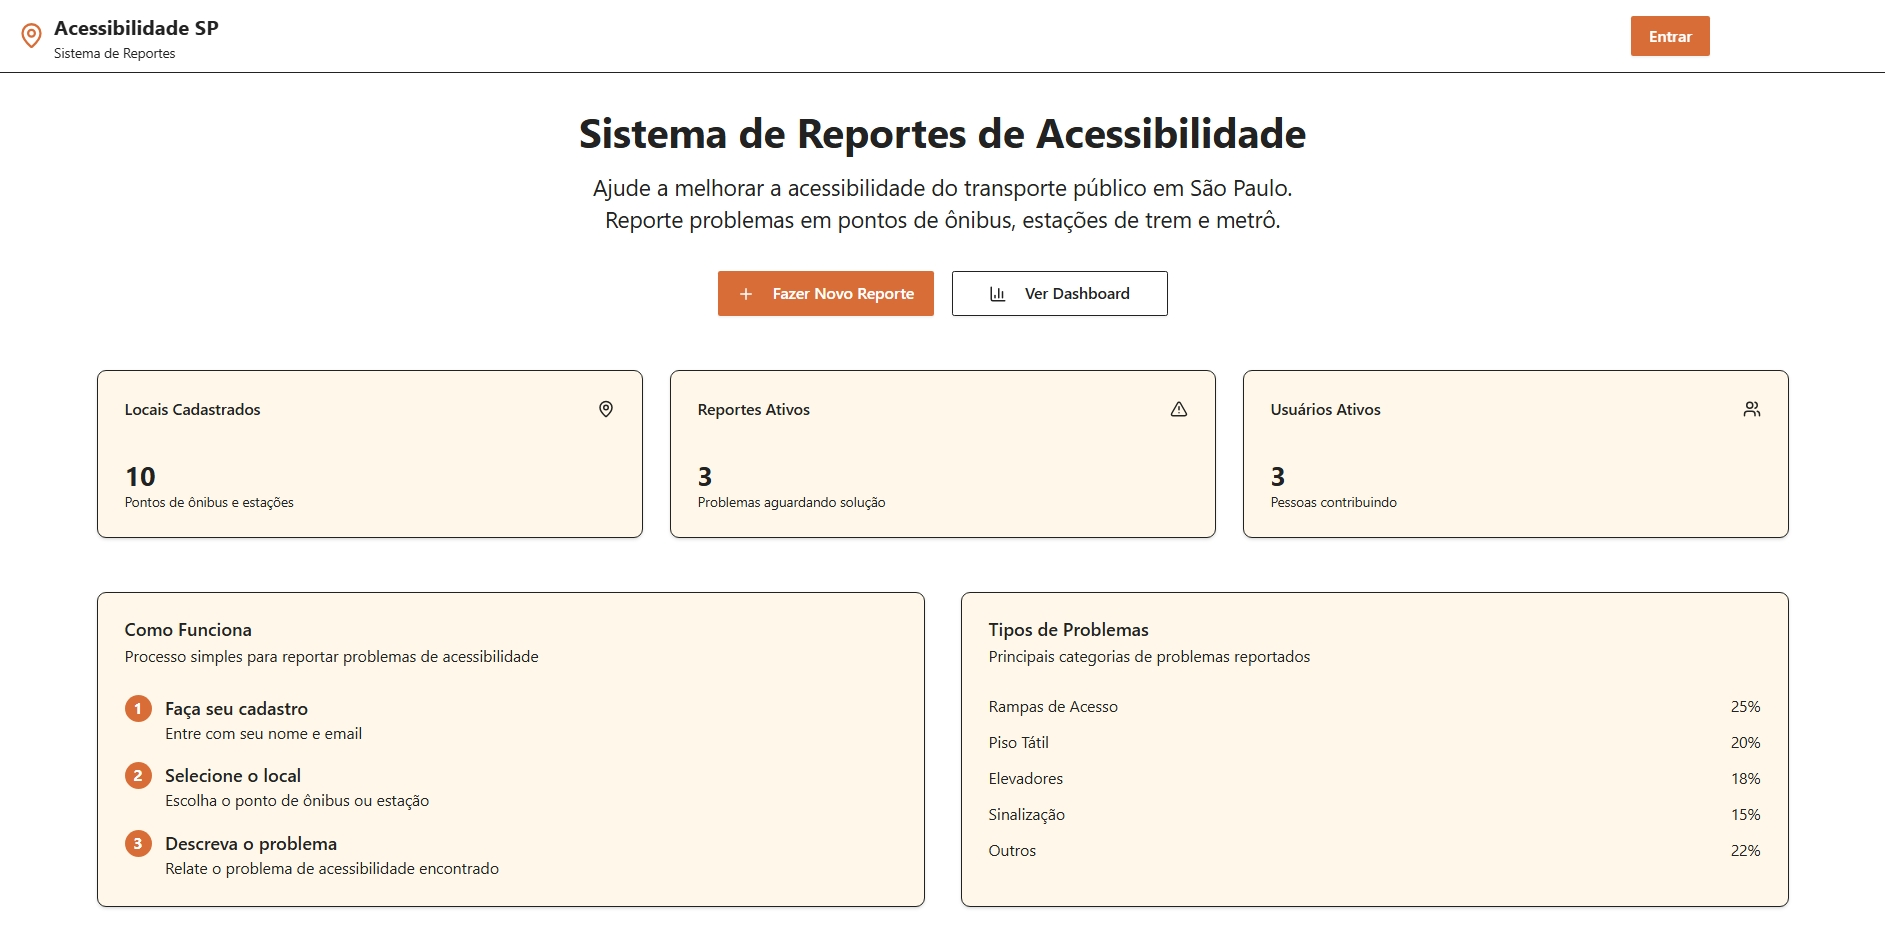
\includegraphics[width=0.8\textwidth]{../imgs/pagina_principal.png}
}{%
    \fbox{\parbox[c][3cm][c]{0.8\textwidth}{\centering Imagem \texttt{pagina\_principal.png} não encontrada}}
}
\caption{Página Principal}
\end{figure}

\subsection{Área do Cliente (Login/Cadastro)}
Tela de acesso ao sistema, onde o usuário entra com nome e e-mail para começar a reportar.

\begin{figure}[H]
\centering
\IfFileExists{../imgs/area_cliente.png}{%
    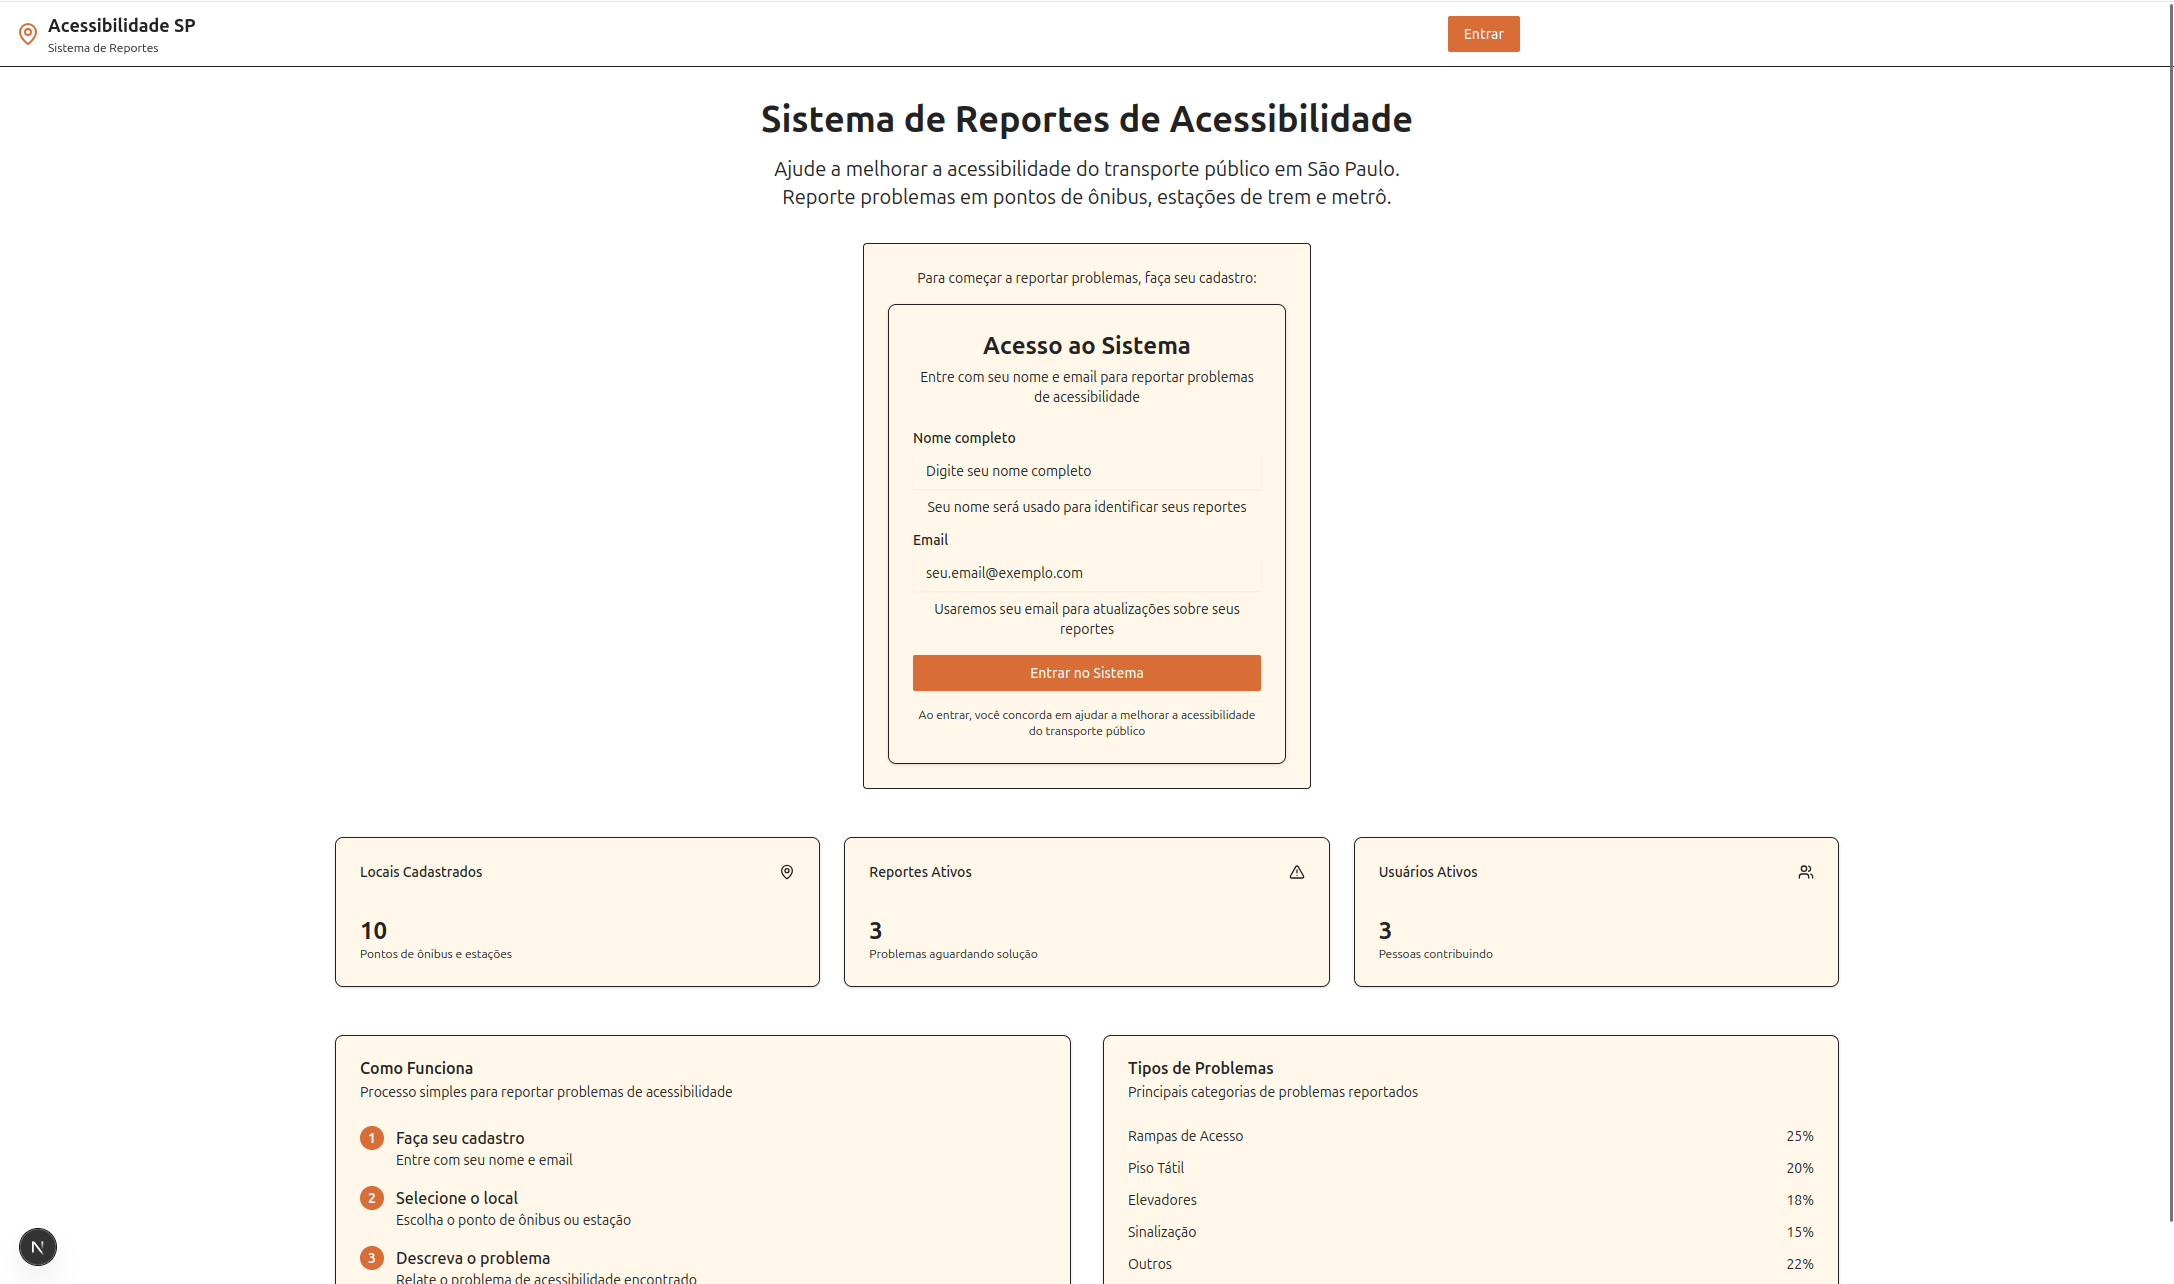
\includegraphics[width=0.8\textwidth]{../imgs/area_cliente.png}
}{%
    \fbox{\parbox[c][3cm][c]{0.8\textwidth}{\centering Imagem \texttt{area\_cliente.png} não encontrada}}
}
\caption{Área do cliente}
\end{figure}

\subsection{Selecionar Local}
Etapa onde o usuário escolhe o ponto de ônibus ou estação onde identificou o problema.

\begin{figure}[H]
\centering
\IfFileExists{../imgs/selecionar_local.png}{%
    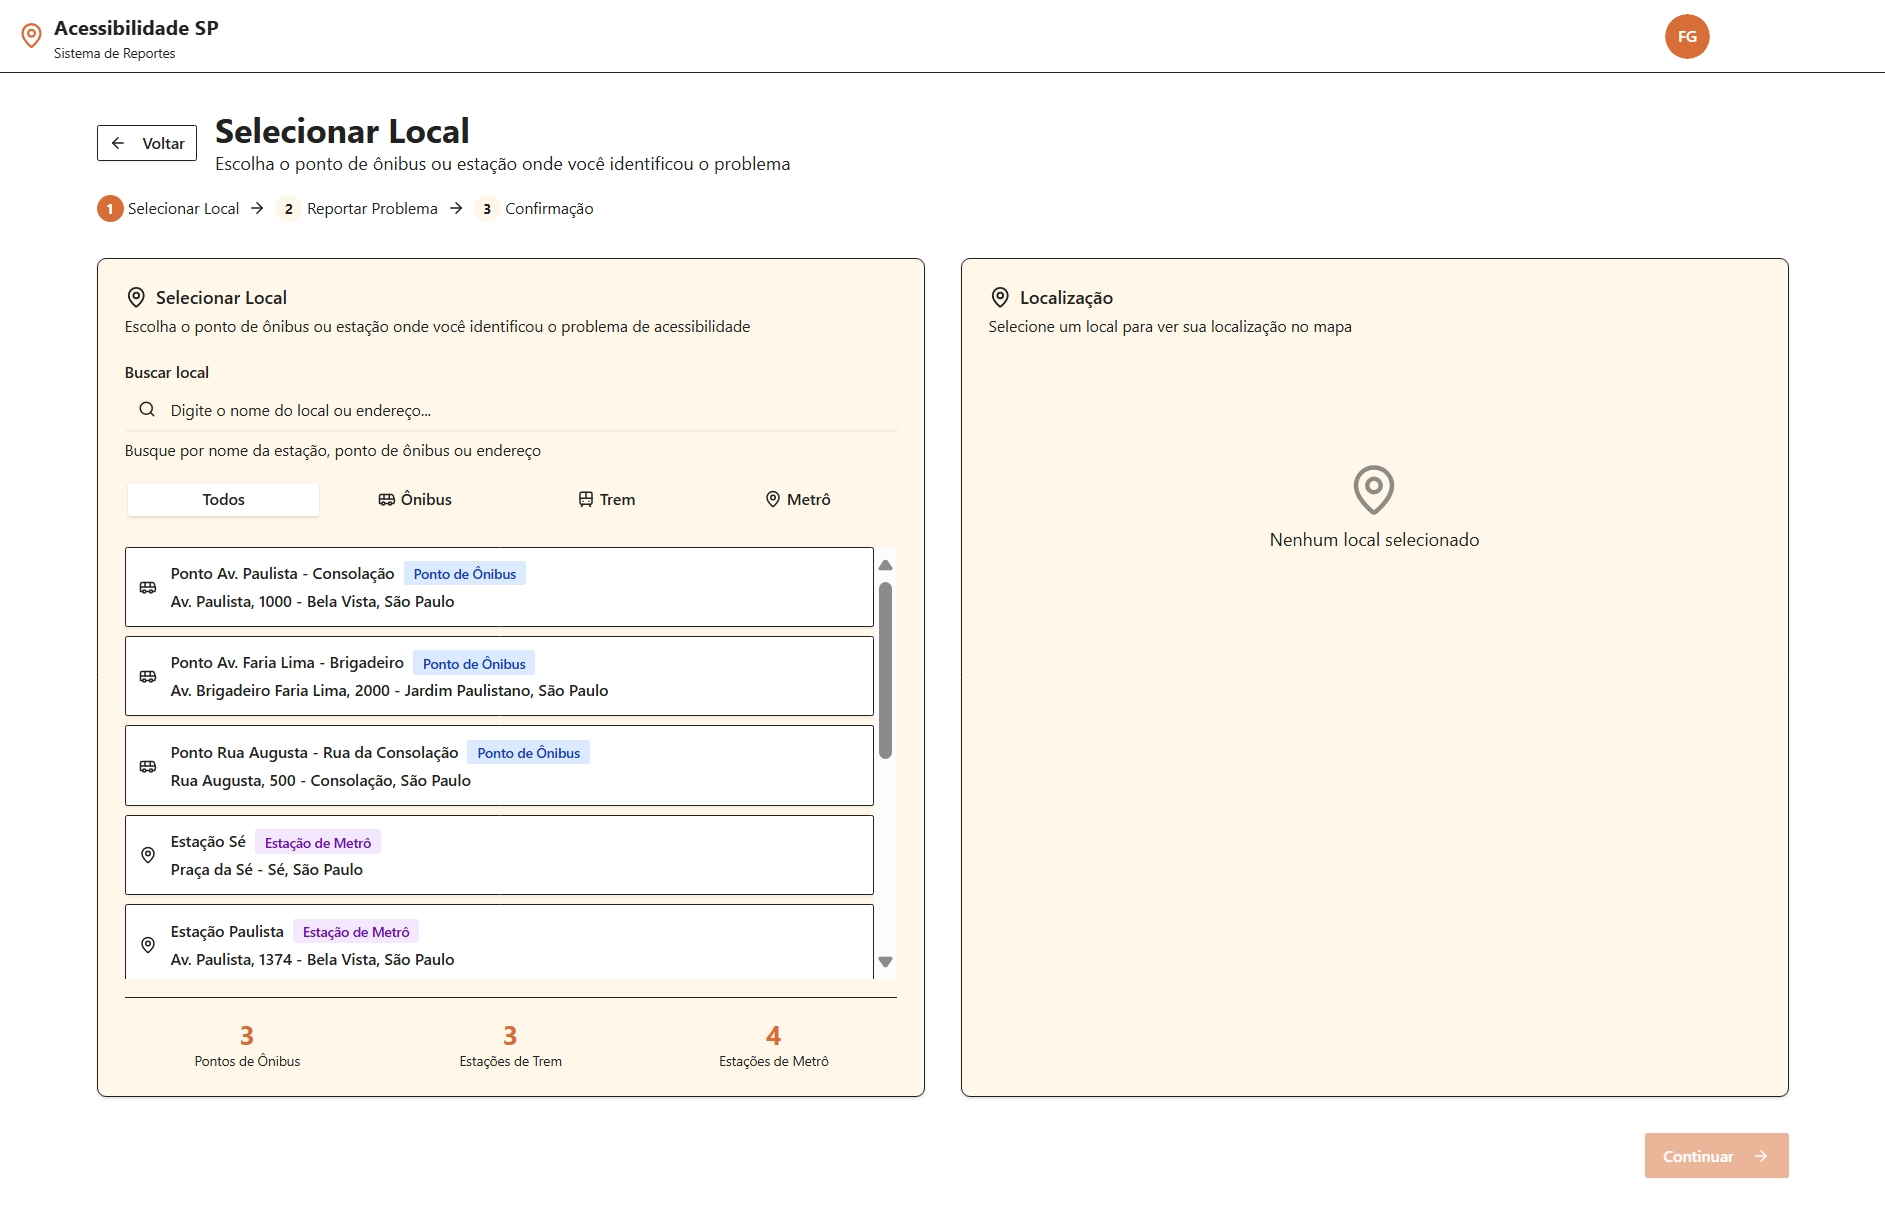
\includegraphics[width=0.8\textwidth]{../imgs/selecionar_local.png}
    }{%
    \fbox{\parbox[c][3cm][c]{0.8\textwidth}{\centering Imagem \texttt{selecionar\_local.png} não encontrada}}
}
\caption{Adicionar um reports}
\end{figure}

\subsection{Reportar Problema – Tipo}
Seleção da categoria do problema (rampa, piso tátil, elevador, etc.).

\begin{figure}[H]
\centering
\IfFileExists{../imgs/reportar_tipo.png}{%
    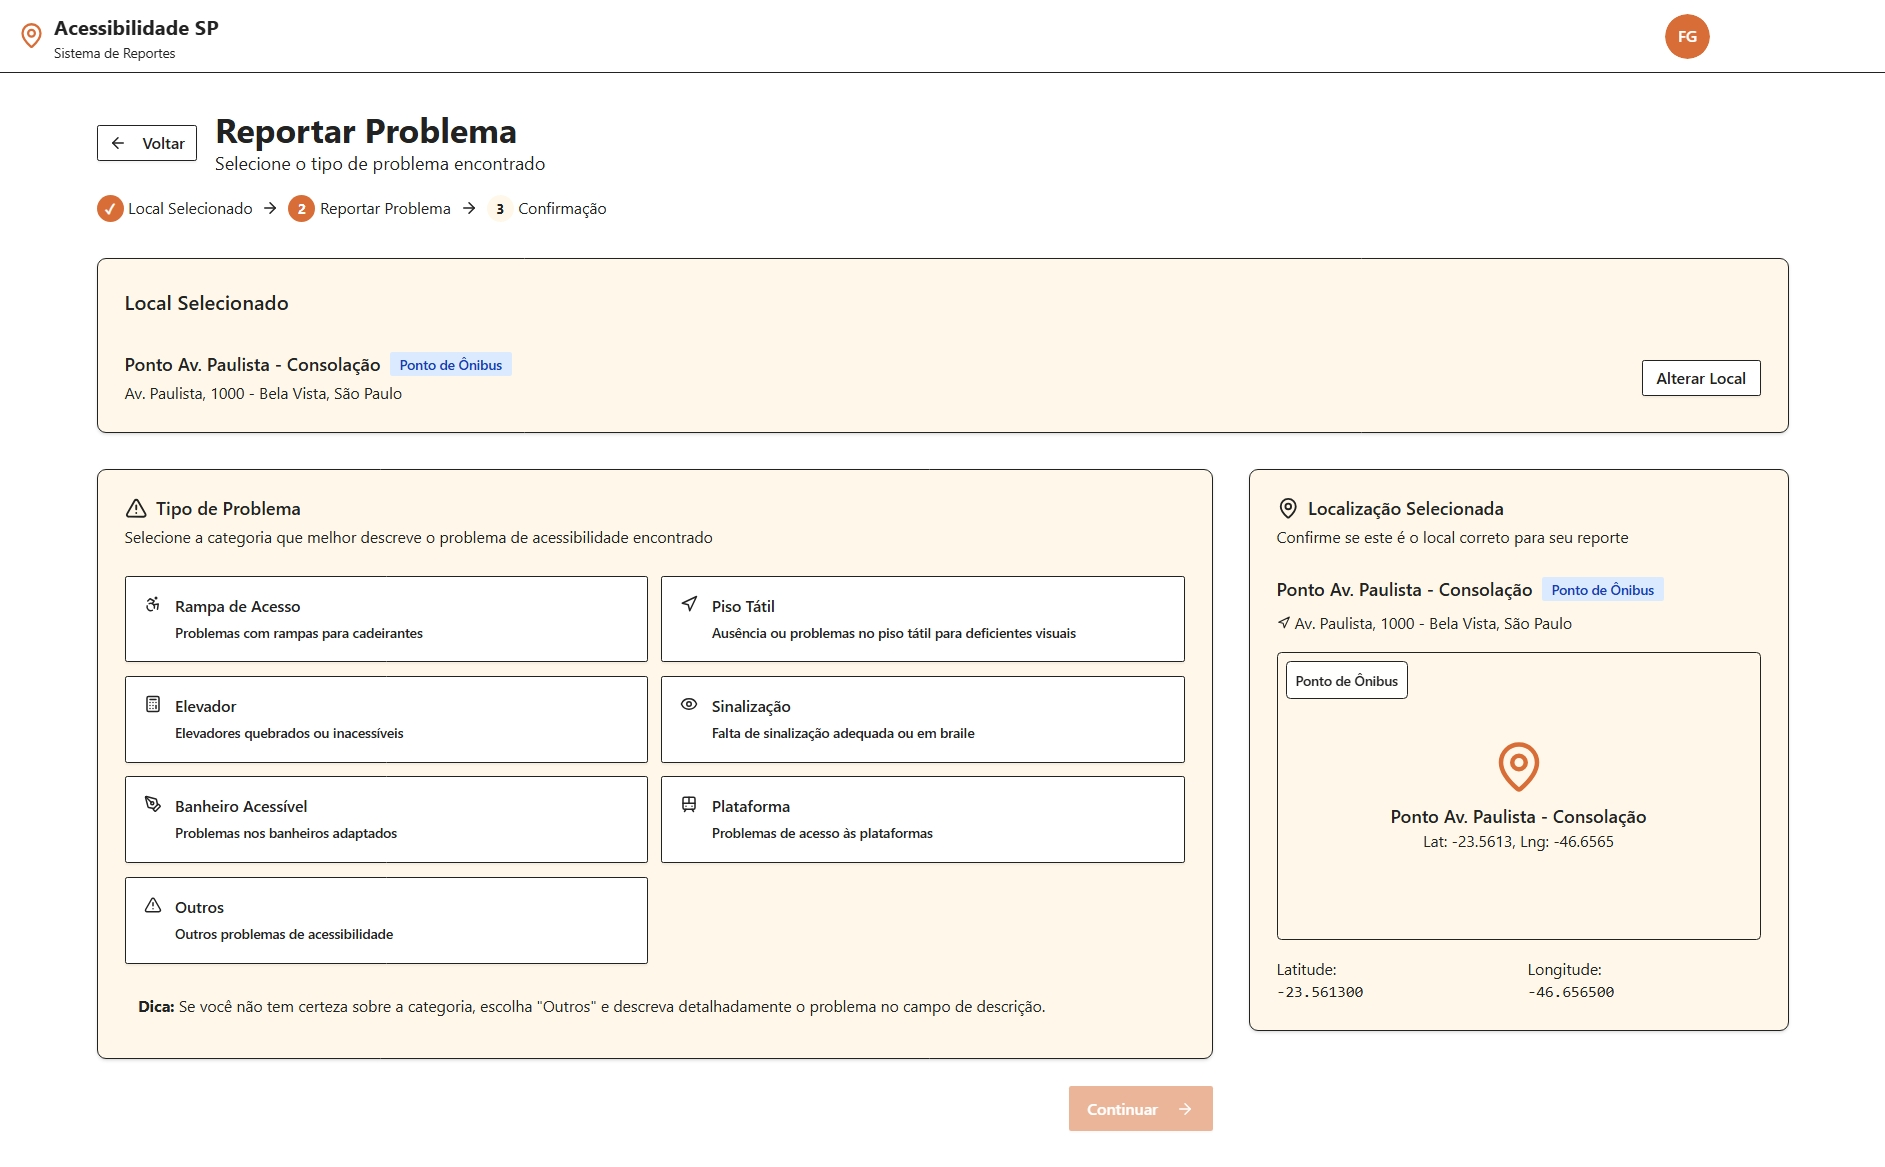
\includegraphics[width=0.8\textwidth]{../imgs/reportar_tipo.png}
}{%
    \fbox{\parbox[c][3cm][c]{0.8\textwidth}{\centering Imagem \texttt{reportar\_tipo.png} não encontrada}}
}
\caption{Reportar problema}
\end{figure}

\subsection{Reportar Problema – Descrição}
Formulário para detalhar o problema, com título e descrição completa.

\begin{figure}[H]
\centering
\IfFileExists{../imgs/reportar_descricao.png}{%
    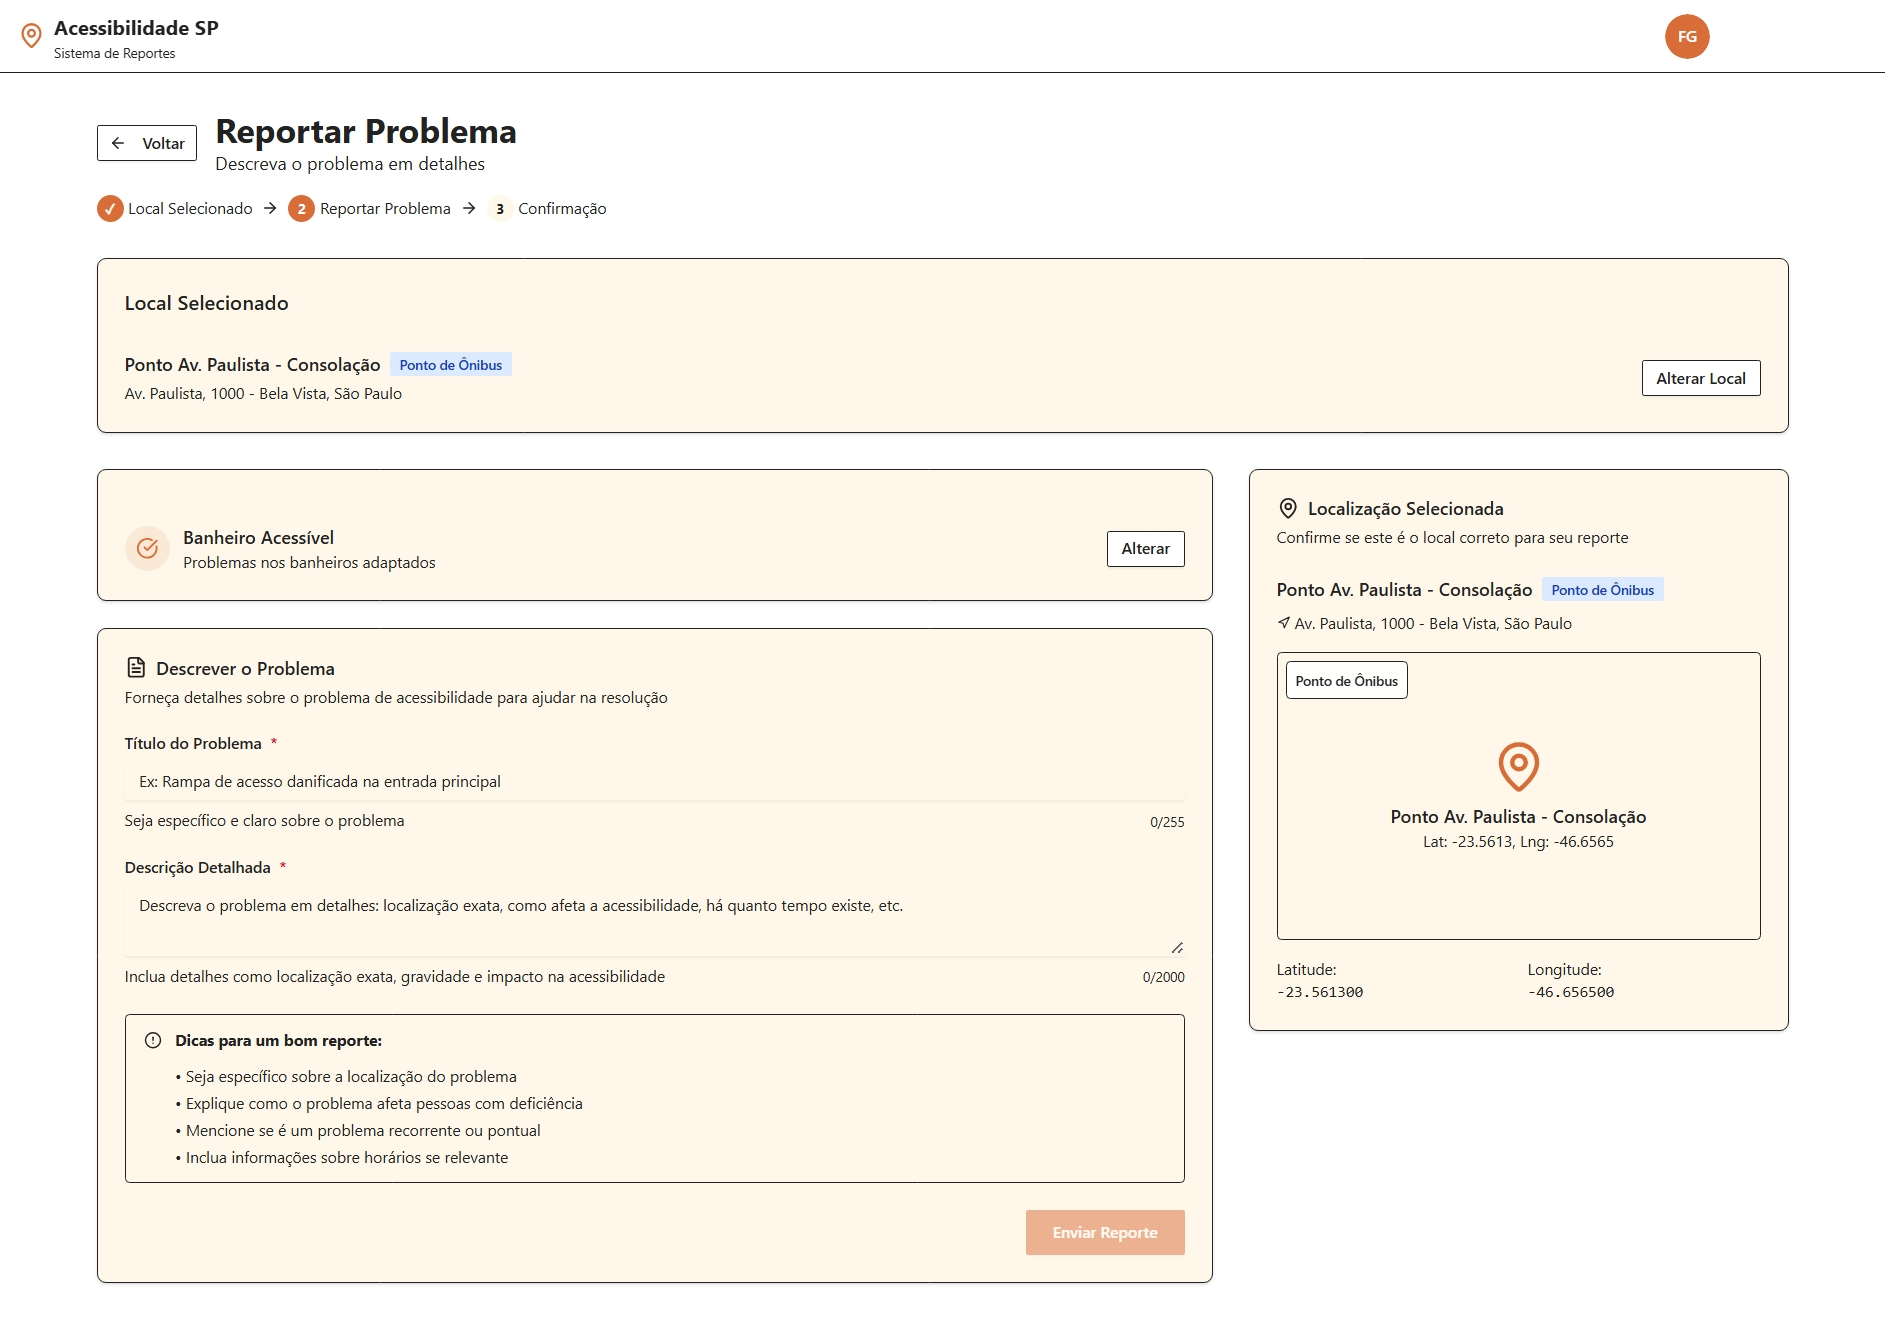
\includegraphics[width=0.8\textwidth]{../imgs/reportar_descricao.png}
}{%
    \fbox{\parbox[c][3cm][c]{0.8\textwidth}{\centering Imagem \texttt{reportar\_descricao.png} não encontrada}}
}
\caption{Descrição do report}
\end{figure}

\subsection{Dashboard – Visão Geral}
Painel com estatísticas globais: número de reports, status, categorias e taxa de resolução.

\begin{figure}[H]
\centering
\IfFileExists{../imgs/dashboard_geral.png}{%
    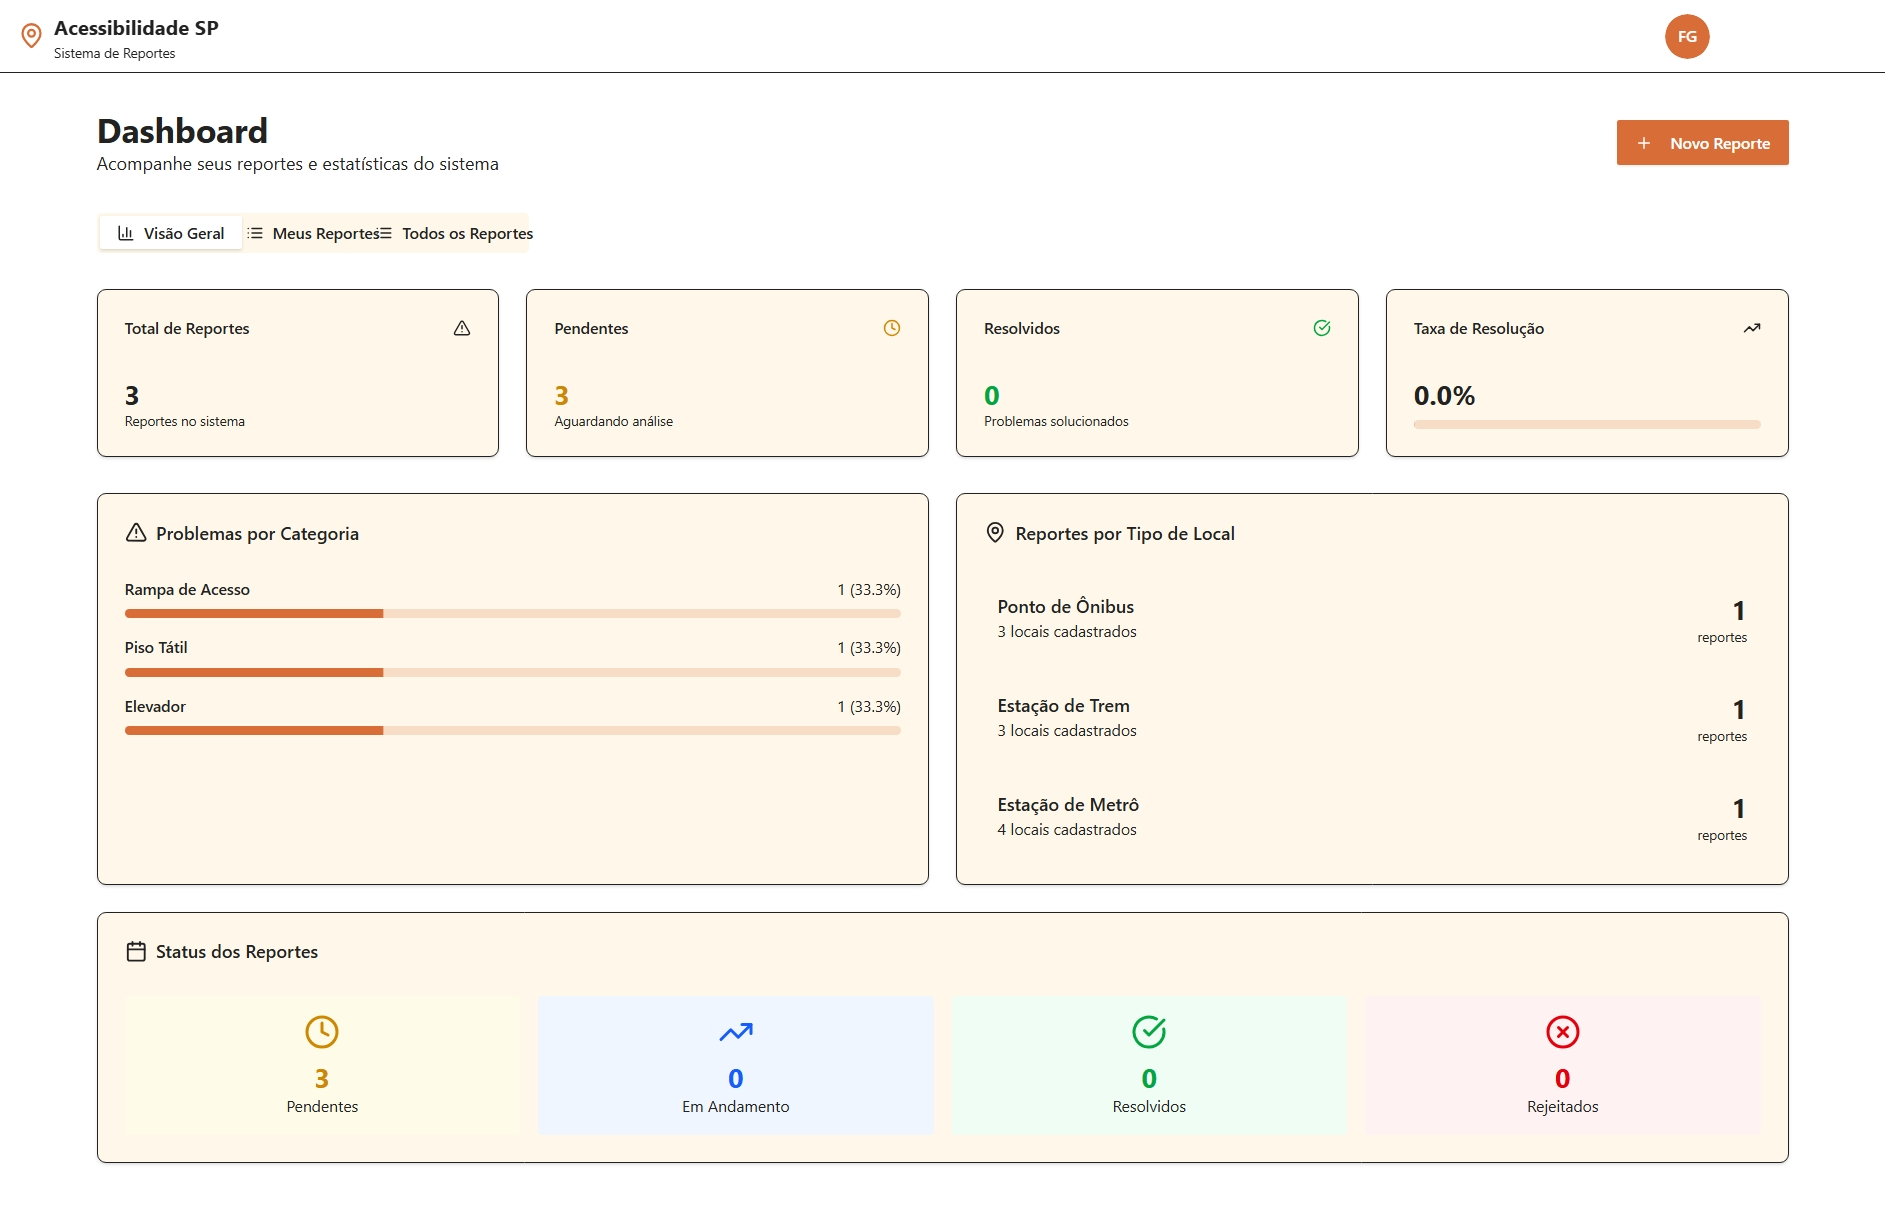
\includegraphics[width=0.8\textwidth]{../imgs/dashboard_geral.png}
}{%
    \fbox{\parbox[c][3cm][c]{0.8\textwidth}{\centering Imagem \texttt{dashboard\_geral.png} não encontrada}}
}
\caption{Dashboards}
\end{figure}

\subsection{Dashboard – Meus Reports}
Lista dos problemas reportados pelo próprio usuário, com seus status.

\begin{figure}[H]
\centering
\IfFileExists{../imgs/dashboard_meus.png}{%
    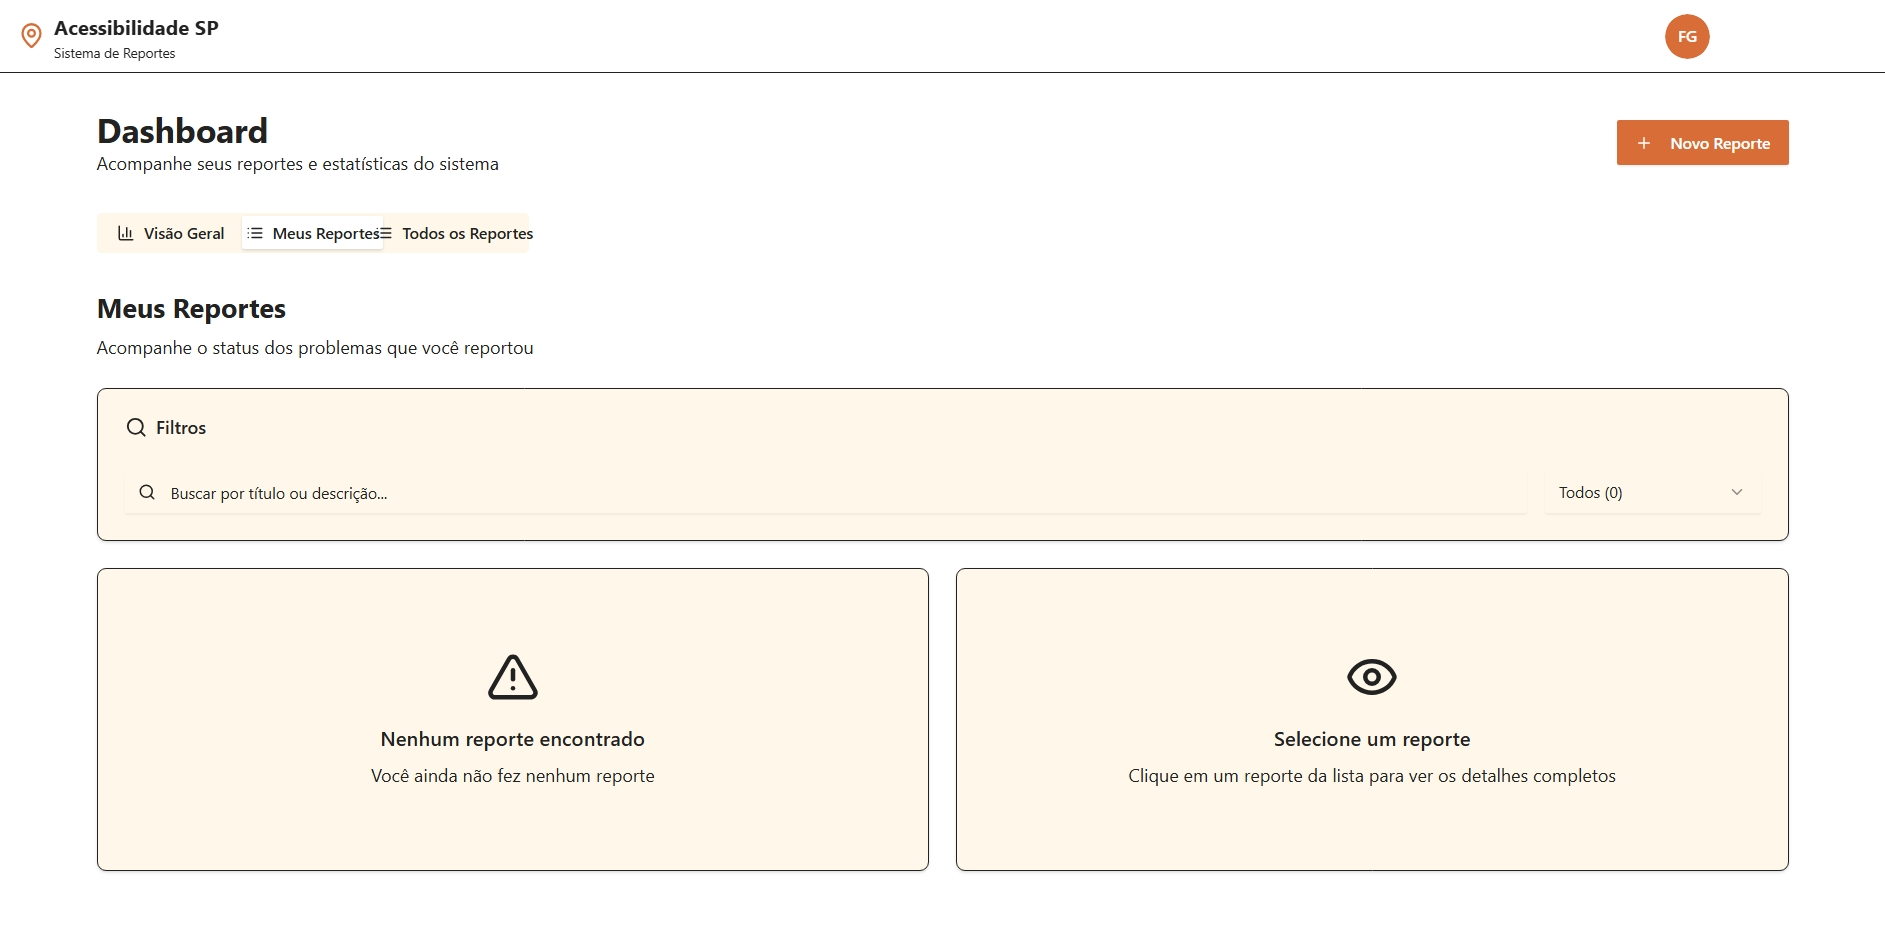
\includegraphics[width=0.8\textwidth]{../imgs/dashboard_meus.png}
}{%
    \fbox{\parbox[c][3cm][c]{0.8\textwidth}{\centering Imagem \texttt{dashboard\_meus.png} não encontrada}}
}
\caption{Dashboards - Meus reports}
\end{figure}

\subsection{Dashboard – Todos os Reports}
Exibe todos os reports do sistema, permitindo visualizar detalhes e acompanhar pendências.

\begin{figure}[H]
\centering
\IfFileExists{../imgs/dashboard_todos.png}{%
    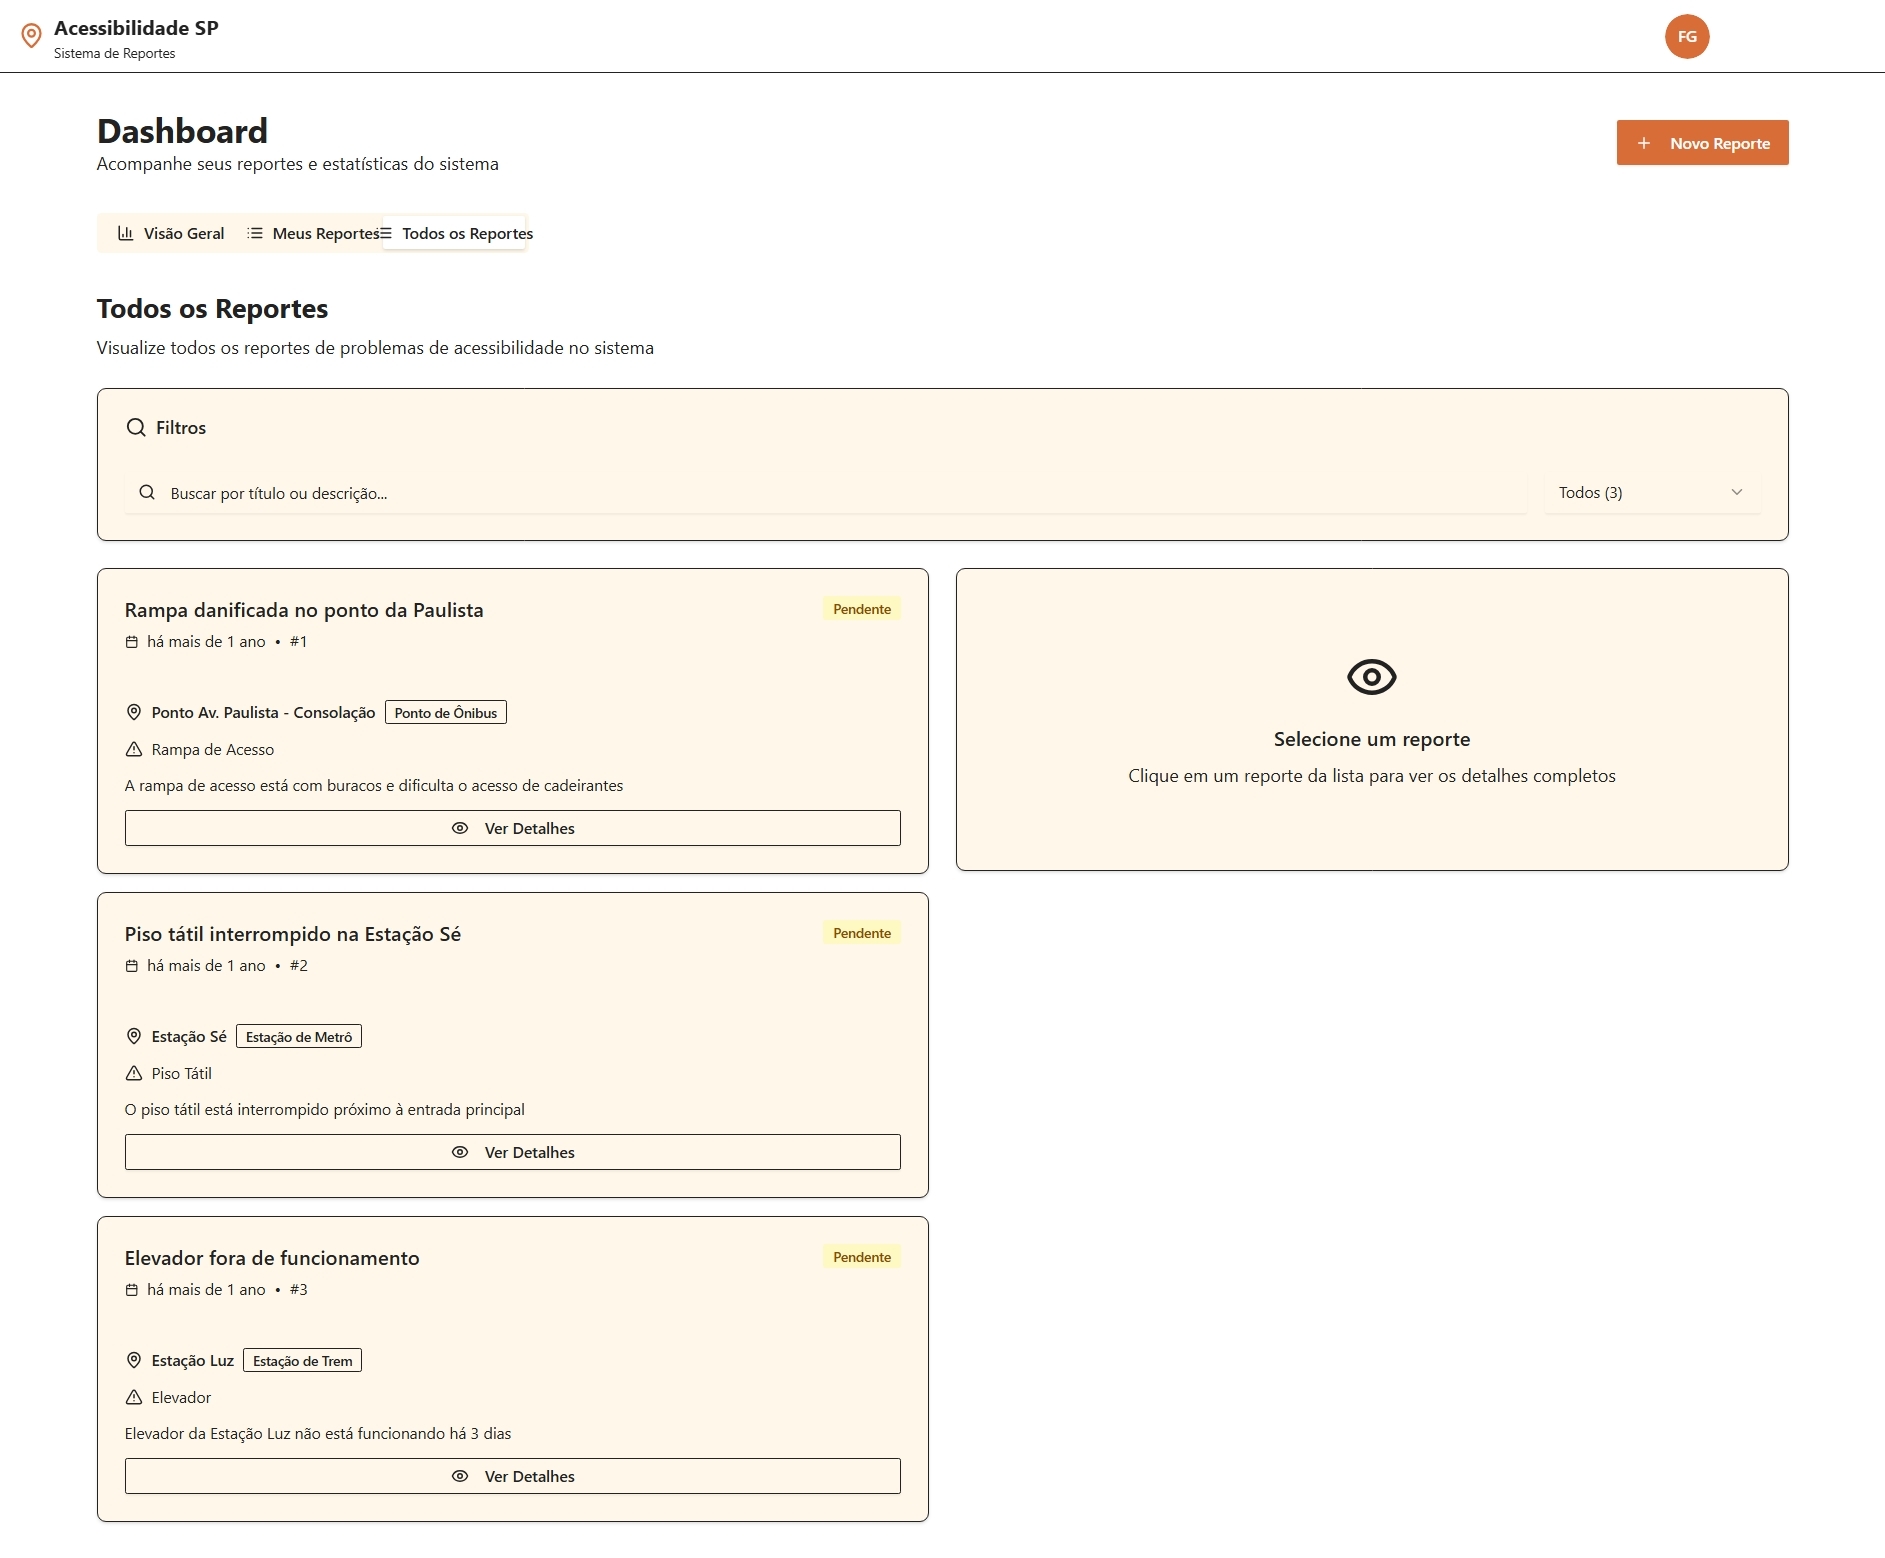
\includegraphics[width=0.8\textwidth]{../imgs/dashboard_todos.png}
}{%
    \fbox{\parbox[c][3cm][c]{0.8\textwidth}{\centering Imagem \texttt{dashboard\_todos.png} não encontrada}}
}
 
\caption{Dashboards - Todos os Reports}
\end{figure}

\section{Modelagem ``Leve do Sistema''}
\label{sec:modelagem}

\subsection{UML - Casos de Uso}

\begin{figure}[H]
\centering
% generated by Plantuml 1.2025.7       
\definecolor{plantucolor0000}{RGB}{0,0,0}
\definecolor{plantucolor0001}{RGB}{241,241,241}
\definecolor{plantucolor0002}{RGB}{24,24,24}
\begin{tikzpicture}[yscale=-1
,pstyle0/.style={color=black,line width=1.5pt}
,pstyle1/.style={color=plantucolor0002,fill=plantucolor0001,line width=0.5pt}
,pstyle2/.style={color=plantucolor0002,line width=0.5pt}
,pstyle3/.style={color=plantucolor0002,line width=1.0pt}
,pstyle4/.style={color=plantucolor0002,fill=plantucolor0002,line width=1.0pt}
]
\draw[pstyle0] (115.5pt,6pt) -- (167.55pt,6pt) arc(270:360:3.75pt)  -- (177.05pt,22pt) -- (287.5pt,22pt) arc(270:360:2.5pt)  -- (290pt,209.5pt) arc(0:90:2.5pt)  -- (115.5pt,212pt) arc(90:180:2.5pt)  -- (113pt,8.5pt) arc(180:270:2.5pt) ;
\draw[pstyle0] (113pt,22pt) -- (177.05pt,22pt);
\node at (117pt,8pt)[below right,color=black,inner sep=0]{\textbf{MoveFácil}};
\draw[pstyle1] (201.6926pt,116.9385pt) ellipse (50.1926pt and 12.4385pt);
\node at (160.0476pt,110.9385pt)[below right,color=black,inner sep=0]{Reportar problema};
\draw[pstyle1] (201.4002pt,179.78pt) ellipse (64.4002pt and 15.28pt);
\node at (144.3702pt,173.67pt)[below right,color=black,inner sep=0]{Atualizar status problema};
\draw[pstyle1] (201.3811pt,51.8762pt) ellipse (72.3811pt and 16.8762pt);
\node at (135.7411pt,45.8212pt)[below right,color=black,inner sep=0]{Consultar mapa de problemas};
\draw[pstyle1] (37.275pt,37.5pt) ellipse (8pt and 8pt);
\draw[pstyle2] (37.275pt,45.5pt) -- (37.275pt,72.5pt)(24.275pt,53.5pt) -- (50.275pt,53.5pt)(37.275pt,72.5pt) -- (24.275pt,87.5pt)(37.275pt,72.5pt) -- (50.275pt,87.5pt);
\node at (14.5pt,89pt)[below right,color=black,inner sep=0]{Passageiro};
\draw[pstyle1] (37.73pt,153.5pt) ellipse (8pt and 8pt);
\draw[pstyle2] (37.73pt,161.5pt) -- (37.73pt,188.5pt)(24.73pt,169.5pt) -- (50.73pt,169.5pt)(37.73pt,188.5pt) -- (24.73pt,203.5pt)(37.73pt,188.5pt) -- (50.73pt,203.5pt);
\node at (6pt,205pt)[below right,color=black,inner sep=0]{Administrador};
\draw[pstyle3] (60.66pt,71.36pt) ..controls (73.58pt,75.65pt) and (90.21pt,81.15pt) .. (105pt,86pt) ..controls (126.7pt,93.11pt) and (145.4917pt,99.212pt) .. (164.2417pt,105.282pt);
\draw[pstyle4] (169.95pt,107.13pt) -- (162.6195pt,100.5525pt) -- (165.1931pt,105.59pt) -- (160.1555pt,108.1636pt) -- (169.95pt,107.13pt) -- cycle;
\draw[pstyle3] (60.69pt,62.36pt) ..controls (79.14pt,60.99pt) and (100.4565pt,59.4143pt) .. (126.0465pt,57.5143pt);
\draw[pstyle4] (132.03pt,57.07pt) -- (122.7585pt,53.7474pt) -- (127.0437pt,57.4402pt) -- (123.3509pt,61.7254pt) -- (132.03pt,57.07pt) -- cycle;
\draw[pstyle3] (69.35pt,180pt) ..controls (88.45pt,180pt) and (107.67pt,180pt) .. (130.89pt,180pt);
\draw[pstyle4] (136.89pt,180pt) -- (127.89pt,176pt) -- (131.89pt,180pt) -- (127.89pt,184pt) -- (136.89pt,180pt) -- cycle;
\end{tikzpicture}

\caption{Diagrama de Casos de Uso}
\end{figure}

\subsubsection{Especificações dos Casos de Uso}

\paragraph{5.1.1.1 Reportar Problema}

\begin{longtable}{|>{\raggedright\arraybackslash}p{3.5cm}|>{\raggedright\arraybackslash}p{10cm}|}
\hline
\textbf{Identificador} & UC001 – Reportar Problema \\
\hline
\textbf{Nome} & Reportar Problema \\
\hline
\textbf{Atores} & Primário: Pedestre utilizando o Sistema de Reportes de Acessibilidade. \newline Secundário: Administrador de um ponto registrado no Sistema. \\
\hline
\textbf{Sumário} & Um pedestre cria na plataforma um reporte para um problema de acessibilidade, visto em ponto de transporte público \\
\hline
\textbf{Complexidade} & Média \\
\hline
\textbf{Regras de Negócio} & - RN001: Apenas usuários autenticados podem registrar reportes. \newline - RN002: Todo reporte deve estar vinculado a um local existente no sistema. \newline - RN003: O reporte deve conter obrigatoriamente um título e uma descrição mínima. \newline - RN004: O sistema deve registrar data, hora e usuário responsável pelo reporte. \newline - RN005: O reporte pode conter evidências (foto ou vídeo), mas estas não são obrigatórias. \newline - RN006: O reporte não pode exceder o limite máximo de caracteres definidos pelo sistema (para título e descrição). \\
\hline
\textbf{Pré-condições} & O pedestre deve possuir informações do problema (foto, vídeo). \newline O pedestre deverá disponibiliza sua localização. \newline O pedestre deve ter um cadastro para registrar um reporte. \\
\hline
\textbf{Pós-condição} & O Sistema terá um reporte com todas as informações do problema registrado em seu banco de dados \newline O Sistema registrará o reporte e atualizará o mapa para que o reporte conste para a localização \\
\hline
\textbf{Pontos de Inclusão} & UC004 – Autenticar Usuário (quando necessário). \\
\hline
\textbf{Pontos de Extensão} & UC005 – Notificar Administrador (para pontos monitorados). \\
\hline
\end{longtable}

\textbf{Fluxo Principal}

\begin{longtable}{|>{\raggedright\arraybackslash}p{7cm}|>{\raggedright\arraybackslash}p{7cm}|}
\hline
\textbf{Ações do Ator} & \textbf{Ações do Sistema} \\
\hline
1. O Pedestre seleciona que deseja reportar um problema na página principal & 2. O Sistema exibe uma listagem dos pontos e estações e o mapa \\
\hline
3. Escolhe a localização através da busca pelo nome ou endereço, ou ainda através do mapa & 4. O Sistema retorna e solicita a confirmação do pedestre para que ele prossiga \\
\hline
5. O pedestre verifica as informações do local selecionado e confirma & 6. O Sistema exibe uma lista de categorias problemas e oferece outro passo de confirmação para o pedestre \\
\hline
7. O pedestre confirma a seleção da categoria e local & 8. O Sistema solicita informações sobre o problema e oferece dicas para que o reporte tenha boa qualidade \\
\hline
9. O Pedestre registra um título para o problema e uma descrição que dê mais detalhes sobre a natureza dele e ao checar as informações envia o reporte & 10. O Sistema informa o envio do reporte e solicita se o pedestre deseja criar um novo reporte ou visualizar o reporte publicado. \\
\hline
\end{longtable}

\textbf{Fluxo Alternativo – Pedestre não está logado no sistema}

\begin{longtable}{|>{\raggedright\arraybackslash}p{7cm}|>{\raggedright\arraybackslash}p{7cm}|}
\hline
\textbf{Ações do Ator} & \textbf{Ações do Sistema} \\
\hline
1a. O pedestre seleciona a opção de reportar sem estar logado & 2a. O Sistema redireciona para a tela de login/cadastro (UC004 – Autenticar Usuário). \\
\hline
3a. Após login/cadastro concluído & 4a. O Sistema retorna ao ponto em que o fluxo principal estava, permitindo prosseguir do passo 3. \\
\hline
\end{longtable}

\textbf{Fluxos de Exceção}

\begin{longtable}{|>{\raggedright\arraybackslash}p{7cm}|>{\raggedright\arraybackslash}p{7cm}|}
\hline
\textbf{Ações do Ator} & \textbf{Ações do Sistema} \\
\hline
1e. O pedestre seleciona uma localização inexistente ou inválida & 2e. O sistema exibe mensagem de erro e solicita nova seleção de localização. \\
\hline
2e. O pedestre não insere título ou descrição & 3e. O sistema informa que os campos são obrigatórios e impede o envio até que sejam preenchidos. \\
\hline
3e. O pedestre tenta anexar arquivo em formato não suportado & 4e. O sistema rejeita o upload e informa quais formatos são permitidos. \\
\hline
4e. O sistema encontra falha de conexão no envio do reporte & 5e. O sistema notifica falha técnica e oferece a opção de salvar localmente para tentar enviar depois. \\
\hline
\end{longtable}

\paragraph{5.1.1.2 Consultar o Mapa de Problemas}

\begin{longtable}{|p{3.5cm}|p{10cm}|}
\hline
\textbf{Identificador} & UC002 – Consultar Mapa de Problemas \\
\hline
\textbf{Nome} & Consultar Mapa de Problemas \\
\hline
\textbf{Atores} & Primário: Pedestre (usuário do sistema). \newline Secundário: Administrador (para análise de ocorrências). \\
\hline
\textbf{Sumário} & O pedestre acessa o sistema para visualizar, no mapa, os problemas de acessibilidade reportados em pontos de transporte público. \\
\hline
\textbf{Complexidade} & Baixa \\
\hline
\textbf{Regras de Negócio} & - RN007: O mapa deve exibir apenas problemas confirmados e devidamente registrados.\newline - RN008: O usuário pode aplicar filtros (categoria, data, status).\newline - RN009: Cada problema deve estar associado a uma localização válida.\newline - RN010: O sistema deve mostrar a data de registro e a situação do problema (pendente, em análise, resolvido).\newline - RN011: Problemas com mais de 1 ano podem ser arquivados, mas ainda disponíveis mediante filtro avançado. \\
\hline
\textbf{Pré-condições} & O sistema deve conter reportes cadastrados.\newline O pedestre precisa ter acesso à plataforma (não é obrigatório login apenas para consulta). \\
\hline
\textbf{Pós-condição} & O usuário terá acesso visual aos problemas existentes no mapa e poderá selecionar pontos para ver detalhes. \\
\hline
\textbf{Pontos de Inclusão} & UC006 – Visualizar Detalhes de Problema (quando o usuário seleciona um ponto específico). \\
\hline
\textbf{Pontos de Extensão} & UC001 – Reportar Problema (usuário pode criar um novo reporte a partir do mapa). \\
\hline
\end{longtable}

\textbf{Fluxo Principal}

\begin{longtable}{|>{\raggedright\arraybackslash}p{7cm}|>{\raggedright\arraybackslash}p{7cm}|}
\hline
\textbf{Ações do Ator} & \textbf{Ações do Sistema} \\
\hline
1. O pedestre acessa a opção "Consultar mapa de problemas". & 2. O sistema carrega o mapa com todos os pontos e marcadores de problemas registrados. \\
\hline
3. O pedestre pode aplicar filtros (categoria, data, status). & 4. O sistema atualiza o mapa exibindo apenas os problemas que atendem ao filtro. \\
\hline
5. O pedestre navega pelo mapa e seleciona um marcador específico. & 6. O sistema exibe informações resumidas do problema e opção de ver detalhes (UC006). \\
\hline
\end{longtable}

\textbf{Fluxo Alternativo – Sem problemas cadastrados}

\begin{longtable}{|>{\raggedright\arraybackslash}p{7cm}|>{\raggedright\arraybackslash}p{7cm}|}
\hline
\textbf{Ações do Ator} & \textbf{Ações do Sistema} \\
\hline
1a. O pedestre acessa o mapa sem que haja reportes cadastrados. & 2a. O sistema exibe mensagem "Nenhum problema cadastrado até o momento" e mostra apenas os pontos sem ocorrências. \\
\hline
\end{longtable}

\textbf{Fluxos de Exceção}

\begin{longtable}{|>{\raggedright\arraybackslash}p{7cm}|>{\raggedright\arraybackslash}p{7cm}|}
\hline
\textbf{Ações do Ator} & \textbf{Ações do Sistema} \\
\hline
1e. O sistema não consegue carregar o mapa (falha na API de mapas ou conexão). & 2e. O sistema exibe mensagem de erro "Não foi possível carregar o mapa. Tente novamente mais tarde". \\
\hline
2e. O usuário aplica um filtro inválido ou inexistente. & 3e. O sistema exibe mensagem "Filtro inválido" e mantém a última visualização correta. \\
\hline
3e. O marcador selecionado não possui dados válidos (erro no registro). & 4e. O sistema exibe mensagem de inconsistência e oculta o marcador defeituoso. \\
\hline
\end{longtable}

\paragraph{5.1.1.3 Atualizar Status de Problema}

\begin{longtable}{|p{3.5cm}|p{10cm}|}
\hline
\textbf{Identificador} & UC003 – Atualizar Status de Problema \\
\hline
\textbf{Nome} & Atualizar Status de Problema \\
\hline
\textbf{Atores} & Primário: Administrador (responsável por um ponto de transporte público). \newline Secundário: Pedestre autor do reporte. \\
\hline
\textbf{Sumário} & O administrador acessa o sistema para alterar o status de um problema reportado, e o pedestre autor do reporte deve confirmar a resolução antes do status ser consolidado como "Resolvido". \\
\hline
\textbf{Complexidade} & Alta \\
\hline
\textbf{Regras de Negócio} & - RN012: Apenas administradores autenticados podem atualizar status.\newline - RN013: O status pode assumir: \textbf{Pendente}, \textbf{Em Análise}, \textbf{Resolvido Provisório}, \textbf{Resolvido Confirmado}, \textbf{Arquivado}.\newline - RN014: Toda atualização deve registrar data, hora e autor da alteração.\newline - RN015: Ao alterar para "Resolvido Provisório", o sistema notifica o pedestre autor para validação.\newline - RN016: O pedestre tem um prazo (ex.: 7 dias) para confirmar a resolução; se não houver resposta, o sistema automaticamente consolida como "Resolvido Confirmado".\newline - RN017: Caso o pedestre rejeite a resolução, o status volta para \textbf{Em Análise}. \\
\hline
\textbf{Pré-condições} & O administrador deve estar autenticado.\newline Deve existir pelo menos um problema reportado no ponto administrado.\newline O pedestre autor deve estar vinculado ao reporte. \\
\hline
\textbf{Pós-condição} & O status do problema será atualizado no sistema, refletindo tanto a ação do administrador quanto a validação do pedestre. \\
\hline
\textbf{Pontos de Inclusão} & UC002 – Consultar Mapa de Problemas (para localizar o problema). \\
\hline
\textbf{Pontos de Extensão} & UC006 – Visualizar Detalhes de Problema (para acompanhar histórico e status detalhado). \\
\hline
\end{longtable}

\textbf{Fluxo Principal}

\begin{longtable}{|>{\raggedright\arraybackslash}p{7cm}|>{\raggedright\arraybackslash}p{7cm}|}
\hline
\textbf{Ações do Ator} & \textbf{Ações do Sistema} \\
\hline
1. O administrador acessa a lista/mapa de problemas reportados. & 2. O sistema exibe os problemas associados ao ponto. \\
\hline
3. O administrador seleciona um problema específico. & 4. O sistema exibe detalhes do problema e status atual. \\
\hline
5. O administrador escolhe a opção de atualizar status para "Resolvido Provisório". & 6. O sistema registra a alteração e envia notificação ao pedestre autor. \\
\hline
7. O pedestre recebe a notificação e abre o problema. & 8. O sistema exibe detalhes da resolução e opções de confirmar ou rejeitar. \\
\hline
9. O pedestre confirma a resolução. & 10. O sistema altera o status para "Resolvido Confirmado", registra histórico e atualiza o mapa. \\
\hline
\end{longtable}

\textbf{Fluxo Alternativo - Pedestre rejeita a resolução}

\begin{longtable}{|>{\raggedright\arraybackslash}p{7cm}|>{\raggedright\arraybackslash}p{7cm}|}
\hline
\textbf{Ações do Ator} & \textbf{Ações do Sistema} \\
\hline
9a. O pedestre rejeita a resolução. & 10a. O sistema altera o status de volta para \textbf{Em Análise} e notifica o administrador. \\
\hline
\end{longtable}

\textbf{Fluxo Alternativo – Pedestre não responde}

\begin{longtable}{|>{\raggedright\arraybackslash}p{7cm}|>{\raggedright\arraybackslash}p{7cm}|}
\hline
\textbf{Ações do Ator} & \textbf{Ações do Sistema} \\
\hline
9b. O pedestre não responde dentro do prazo (ex.: 7 dias). & 10b. O sistema consolida automaticamente o status como \textbf{Resolvido Confirmado} e registra no histórico. \\
\hline
\end{longtable}

\textbf{Fluxo de Exceção}

% Ajuste: usar raggedright nas colunas desta longtable de exceção
\begin{longtable}{|>{\raggedright\arraybackslash}p{7cm}|>{\raggedright\arraybackslash}p{7cm}|}
\hline
\textbf{Ações do Ator} & \textbf{Ações do Sistema} \\
\hline
1e. O administrador não está autenticado. & 2e. O sistema bloqueia e redireciona para login. \\
\hline
2e. O pedestre não consegue abrir o reporte (erro técnico). & 3e. O sistema exibe mensagem de erro e orienta tentar novamente. \\
\hline
3e. O administrador tenta alterar status de problema fora de sua jurisdição. & 4e. O sistema impede a ação e informa falta de permissão. \\
\hline
\end{longtable}

\subsection{UML - Diagrama de Classe de Domínio}

\begin{figure}[H]
\centering
% generated by Plantuml 1.2025.7       
\definecolor{plantucolor0000}{RGB}{241,241,241}
\definecolor{plantucolor0001}{RGB}{24,24,24}
\definecolor{plantucolor0002}{RGB}{169,220,223}
\definecolor{plantucolor0003}{RGB}{0,0,0}
\definecolor{plantucolor0004}{RGB}{173,209,178}
\definecolor{plantucolor0005}{RGB}{235,147,127}
\begin{tikzpicture}[yscale=-1
,pstyle0/.style={color=plantucolor0001,fill=plantucolor0000,line width=0.5pt}
,pstyle1/.style={color=plantucolor0001,fill=plantucolor0002,line width=1.0pt}
,pstyle2/.style={color=plantucolor0001,line width=0.5pt}
,pstyle3/.style={color=plantucolor0001,fill=plantucolor0004,line width=1.0pt}
,pstyle4/.style={color=plantucolor0001,fill=plantucolor0005,line width=1.0pt}
,pstyle5/.style={color=plantucolor0001,line width=1.0pt}
]
\draw[pstyle0] (565pt,212pt) arc (180:270:5pt) -- (570pt,207pt) -- (683.67pt,207pt) arc (270:360:5pt) -- (688.67pt,212pt) -- (688.67pt,300pt) arc (0:90:5pt) -- (683.67pt,305pt) -- (570pt,305pt) arc (90:180:5pt) -- (565pt,300pt) -- cycle;
\draw[pstyle1] (606.001pt,223pt) ellipse (11pt and 11pt);
\node at (606.001pt,223pt)[]{\textbf{\Large A}};
\node at (625.779pt,218pt)[below right,color=black,inner sep=0]{\textit{Usuario}};
\draw[pstyle2] (566pt,239pt) -- (687.67pt,239pt);
\node at (571pt,243pt)[below right,color=black,inner sep=0]{+id: UUID};
\node at (571pt,253pt)[below right,color=black,inner sep=0]{+nome: string};
\node at (571pt,263pt)[below right,color=black,inner sep=0]{+email: string};
\node at (571pt,273pt)[below right,color=black,inner sep=0]{+senhaHash: string};
\node at (571pt,283pt)[below right,color=black,inner sep=0]{+ultimoLogin: DateTime};
\draw[pstyle2] (566pt,297pt) -- (687.67pt,297pt);
\draw[pstyle0] (582pt,386pt) arc (180:270:5pt) -- (587pt,381pt) -- (667.42pt,381pt) arc (270:360:5pt) -- (672.42pt,386pt) -- (672.42pt,444pt) arc (0:90:5pt) -- (667.42pt,449pt) -- (587pt,449pt) arc (90:180:5pt) -- (582pt,444pt) -- cycle;
\draw[pstyle3] (602.7915pt,397pt) ellipse (11pt and 11pt);
\node at (602.7915pt,397pt)[]{\textbf{\Large C}};
\node at (618.0785pt,392pt)[below right,color=black,inner sep=0]{Passageiro};
\draw[pstyle2] (583pt,413pt) -- (671.42pt,413pt);
\node at (588pt,417pt)[below right,color=black,inner sep=0]{+cpf: string};
\node at (588pt,427pt)[below right,color=black,inner sep=0]{+telefone?: string};
\draw[pstyle2] (583pt,441pt) -- (671.42pt,441pt);
\draw[pstyle0] (421.5pt,576pt) arc (180:270:5pt) -- (426.5pt,571pt) -- (511.96pt,571pt) arc (270:360:5pt) -- (516.96pt,576pt) -- (516.96pt,634pt) arc (0:90:5pt) -- (511.96pt,639pt) -- (426.5pt,639pt) arc (90:180:5pt) -- (421.5pt,634pt) -- cycle;
\draw[pstyle3] (436.5pt,587pt) ellipse (11pt and 11pt);
\node at (436.5pt,587pt)[]{\textbf{\Large C}};
\node at (450.5pt,582pt)[below right,color=black,inner sep=0]{Administrador};
\draw[pstyle2] (422.5pt,603pt) -- (515.96pt,603pt);
\node at (427.5pt,607pt)[below right,color=black,inner sep=0]{+cargo: string};
\node at (427.5pt,617pt)[below right,color=black,inner sep=0]{+ativo: boolean};
\draw[pstyle2] (422.5pt,631pt) -- (515.96pt,631pt);
\draw[pstyle0] (128.5pt,371pt) arc (180:270:5pt) -- (133.5pt,366pt) -- (262.44pt,366pt) arc (270:360:5pt) -- (267.44pt,371pt) -- (267.44pt,459pt) arc (0:90:5pt) -- (262.44pt,464pt) -- (133.5pt,464pt) arc (90:180:5pt) -- (128.5pt,459pt) -- cycle;
\draw[pstyle3] (143.5pt,382pt) ellipse (11pt and 11pt);
\node at (143.5pt,382pt)[]{\textbf{\Large C}};
\node at (157.5pt,377pt)[below right,color=black,inner sep=0]{OrganizacaoResponsavel};
\draw[pstyle2] (129.5pt,398pt) -- (266.44pt,398pt);
\node at (134.5pt,402pt)[below right,color=black,inner sep=0]{+id: UUID};
\node at (134.5pt,412pt)[below right,color=black,inner sep=0]{+nome: string};
\node at (134.5pt,422pt)[below right,color=black,inner sep=0]{+cnpj: string};
\node at (134.5pt,432pt)[below right,color=black,inner sep=0]{+tipo: string};
\node at (134.5pt,442pt)[below right,color=black,inner sep=0]{+contatoPrincipal: string};
\draw[pstyle2] (129.5pt,456pt) -- (266.44pt,456pt);
\draw[pstyle0] (121.5pt,751pt) arc (180:270:5pt) -- (126.5pt,746pt) -- (217.4pt,746pt) arc (270:360:5pt) -- (222.4pt,751pt) -- (222.4pt,849pt) arc (0:90:5pt) -- (217.4pt,854pt) -- (126.5pt,854pt) arc (90:180:5pt) -- (121.5pt,849pt) -- cycle;
\draw[pstyle1] (145.59pt,762pt) ellipse (11pt and 11pt);
\node at (145.59pt,762pt)[]{\textbf{\Large A}};
\node at (161.61pt,757pt)[below right,color=black,inner sep=0]{\textit{Localizacao}};
\draw[pstyle2] (122.5pt,778pt) -- (221.4pt,778pt);
\node at (127.5pt,782pt)[below right,color=black,inner sep=0]{+id: UUID};
\node at (127.5pt,792pt)[below right,color=black,inner sep=0]{+nome: string};
\node at (127.5pt,802pt)[below right,color=black,inner sep=0]{+descricao: string};
\node at (127.5pt,812pt)[below right,color=black,inner sep=0]{+endereco: string};
\node at (127.5pt,822pt)[below right,color=black,inner sep=0]{+latitude: decimal};
\node at (127.5pt,832pt)[below right,color=black,inner sep=0]{+longitude: decimal};
\draw[pstyle2] (122.5pt,846pt) -- (221.4pt,846pt);
\draw[pstyle0] (61pt,576pt) arc (180:270:5pt) -- (66pt,571pt) -- (179.78pt,571pt) arc (270:360:5pt) -- (184.78pt,576pt) -- (184.78pt,634pt) arc (0:90:5pt) -- (179.78pt,639pt) -- (66pt,639pt) arc (90:180:5pt) -- (61pt,634pt) -- cycle;
\draw[pstyle3] (91.705pt,587pt) ellipse (11pt and 11pt);
\node at (91.705pt,587pt)[]{\textbf{\Large C}};
\node at (109.195pt,582pt)[below right,color=black,inner sep=0]{PontoOnibus};
\draw[pstyle2] (62pt,603pt) -- (183.78pt,603pt);
\node at (67pt,607pt)[below right,color=black,inner sep=0]{+codigoMunicipal: string};
\node at (67pt,617pt)[below right,color=black,inner sep=0]{+sentido: string};
\draw[pstyle2] (62pt,631pt) -- (183.78pt,631pt);
\draw[pstyle0] (220pt,571pt) arc (180:270:5pt) -- (225pt,566pt) -- (380.66pt,566pt) arc (270:360:5pt) -- (385.66pt,571pt) -- (385.66pt,639pt) arc (0:90:5pt) -- (380.66pt,644pt) -- (225pt,644pt) arc (90:180:5pt) -- (220pt,639pt) -- cycle;
\draw[pstyle3] (268.33pt,582pt) ellipse (11pt and 11pt);
\node at (268.33pt,582pt)[]{\textbf{\Large C}};
\node at (288.83pt,577pt)[below right,color=black,inner sep=0]{EstacaoMetro};
\draw[pstyle2] (221pt,598pt) -- (384.66pt,598pt);
\node at (226pt,602pt)[below right,color=black,inner sep=0]{+linha: string};
\node at (226pt,612pt)[below right,color=black,inner sep=0]{+plataforma: string};
\node at (226pt,622pt)[below right,color=black,inner sep=0]{+acessibilidadeDisponivel: boolean};
\draw[pstyle2] (221pt,636pt) -- (384.66pt,636pt);
\draw[pstyle0] (552pt,541pt) arc (180:270:5pt) -- (557pt,536pt) -- (697.19pt,536pt) arc (270:360:5pt) -- (702.19pt,541pt) -- (702.19pt,669pt) arc (0:90:5pt) -- (697.19pt,674pt) -- (557pt,674pt) arc (90:180:5pt) -- (552pt,669pt) -- cycle;
\draw[pstyle3] (592.1145pt,552pt) ellipse (11pt and 11pt);
\node at (592.1145pt,552pt)[]{\textbf{\Large C}};
\node at (611.6955pt,547pt)[below right,color=black,inner sep=0]{TicketReporte};
\draw[pstyle2] (553pt,568pt) -- (701.19pt,568pt);
\node at (558pt,572pt)[below right,color=black,inner sep=0]{+id: UUID};
\node at (558pt,582pt)[below right,color=black,inner sep=0]{+titulo: string};
\node at (558pt,592pt)[below right,color=black,inner sep=0]{+descricao: string};
\node at (558pt,602pt)[below right,color=black,inner sep=0]{+dataCriacao: DateTime};
\node at (558pt,612pt)[below right,color=black,inner sep=0]{+dataFechamento?: DateTime};
\node at (558pt,622pt)[below right,color=black,inner sep=0]{+statusAtual: Status};
\node at (558pt,632pt)[below right,color=black,inner sep=0]{+gravidade: Gravidade};
\node at (558pt,642pt)[below right,color=black,inner sep=0]{+ultimaAtualizacao: DateTime};
\node at (558pt,652pt)[below right,color=black,inner sep=0]{+qtdConfirmacoes: int};
\draw[pstyle2] (553pt,666pt) -- (701.19pt,666pt);
\draw[pstyle0] (494.5pt,761pt) arc (180:270:5pt) -- (499.5pt,756pt) -- (614.99pt,756pt) arc (270:360:5pt) -- (619.99pt,761pt) -- (619.99pt,839pt) arc (0:90:5pt) -- (614.99pt,844pt) -- (499.5pt,844pt) arc (90:180:5pt) -- (494.5pt,839pt) -- cycle;
\draw[pstyle3] (513.73pt,772pt) ellipse (11pt and 11pt);
\node at (513.73pt,772pt)[]{\textbf{\Large C}};
\node at (528.67pt,767pt)[below right,color=black,inner sep=0]{CategoriaProblema};
\draw[pstyle2] (495.5pt,788pt) -- (618.99pt,788pt);
\node at (500.5pt,792pt)[below right,color=black,inner sep=0]{+id: UUID};
\node at (500.5pt,802pt)[below right,color=black,inner sep=0]{+nome: string};
\node at (500.5pt,812pt)[below right,color=black,inner sep=0]{+descricao: string};
\node at (500.5pt,822pt)[below right,color=black,inner sep=0]{+exigeEvidencia: boolean};
\draw[pstyle2] (495.5pt,836pt) -- (618.99pt,836pt);
\draw[pstyle0] (655pt,761pt) arc (180:270:5pt) -- (660pt,756pt) -- (742.3pt,756pt) arc (270:360:5pt) -- (747.3pt,761pt) -- (747.3pt,839pt) arc (0:90:5pt) -- (742.3pt,844pt) -- (660pt,844pt) arc (90:180:5pt) -- (655pt,839pt) -- cycle;
\draw[pstyle3] (677.9425pt,772pt) ellipse (11pt and 11pt);
\node at (677.9425pt,772pt)[]{\textbf{\Large C}};
\node at (693.7075pt,767pt)[below right,color=black,inner sep=0]{Evidencia};
\draw[pstyle2] (656pt,788pt) -- (746.3pt,788pt);
\node at (661pt,792pt)[below right,color=black,inner sep=0]{+id: UUID};
\node at (661pt,802pt)[below right,color=black,inner sep=0]{+tipo: MediaTipo};
\node at (661pt,812pt)[below right,color=black,inner sep=0]{+url: string};
\node at (661pt,822pt)[below right,color=black,inner sep=0]{+tamanhoKB: int};
\draw[pstyle2] (656pt,836pt) -- (746.3pt,836pt);
\draw[pstyle0] (782pt,761pt) arc (180:270:5pt) -- (787pt,756pt) -- (900.55pt,756pt) arc (270:360:5pt) -- (905.55pt,761pt) -- (905.55pt,839pt) arc (0:90:5pt) -- (900.55pt,844pt) -- (787pt,844pt) arc (90:180:5pt) -- (782pt,839pt) -- cycle;
\draw[pstyle3] (815.3105pt,772pt) ellipse (11pt and 11pt);
\node at (815.3105pt,772pt)[]{\textbf{\Large C}};
\node at (833.3795pt,767pt)[below right,color=black,inner sep=0]{Comentario};
\draw[pstyle2] (783pt,788pt) -- (904.55pt,788pt);
\node at (788pt,792pt)[below right,color=black,inner sep=0]{+id: UUID};
\node at (788pt,802pt)[below right,color=black,inner sep=0]{+conteudo: string};
\node at (788pt,812pt)[below right,color=black,inner sep=0]{+dataCriacao: DateTime};
\node at (788pt,822pt)[below right,color=black,inner sep=0]{+privado: boolean};
\draw[pstyle2] (783pt,836pt) -- (904.55pt,836pt);
\draw[pstyle0] (324pt,756pt) arc (180:270:5pt) -- (329pt,751pt) -- (436.79pt,751pt) arc (270:360:5pt) -- (441.79pt,756pt) -- (441.79pt,844pt) arc (0:90:5pt) -- (436.79pt,849pt) -- (329pt,849pt) arc (90:180:5pt) -- (324pt,844pt) -- cycle;
\draw[pstyle3] (347.415pt,767pt) ellipse (11pt and 11pt);
\node at (347.415pt,767pt)[]{\textbf{\Large C}};
\node at (363.285pt,762pt)[below right,color=black,inner sep=0]{HistoricoStatus};
\draw[pstyle2] (325pt,783pt) -- (440.79pt,783pt);
\node at (330pt,787pt)[below right,color=black,inner sep=0]{+id: UUID};
\node at (330pt,797pt)[below right,color=black,inner sep=0]{+dataHora: DateTime};
\node at (330pt,807pt)[below right,color=black,inner sep=0]{+statusAnterior: Status};
\node at (330pt,817pt)[below right,color=black,inner sep=0]{+statusAtual: Status};
\node at (330pt,827pt)[below right,color=black,inner sep=0]{+justificativa: string};
\draw[pstyle2] (325pt,841pt) -- (440.79pt,841pt);
\draw[pstyle0] (565pt,27pt) arc (180:270:5pt) -- (570pt,22pt) -- (683.95pt,22pt) arc (270:360:5pt) -- (688.95pt,27pt) -- (688.95pt,115pt) arc (0:90:5pt) -- (683.95pt,120pt) -- (570pt,120pt) arc (90:180:5pt) -- (565pt,115pt) -- cycle;
\draw[pstyle3] (599.503pt,38pt) ellipse (11pt and 11pt);
\node at (599.503pt,38pt)[]{\textbf{\Large C}};
\node at (617.837pt,33pt)[below right,color=black,inner sep=0]{Notificacao};
\draw[pstyle2] (566pt,54pt) -- (687.95pt,54pt);
\node at (571pt,58pt)[below right,color=black,inner sep=0]{+id: UUID};
\node at (571pt,68pt)[below right,color=black,inner sep=0]{+mensagem: string};
\node at (571pt,78pt)[below right,color=black,inner sep=0]{+dataEnvio: DateTime};
\node at (571pt,88pt)[below right,color=black,inner sep=0]{+lida: boolean};
\node at (571pt,98pt)[below right,color=black,inner sep=0]{+canal: CanalNotificacao};
\draw[pstyle2] (566pt,112pt) -- (687.95pt,112pt);
\draw[pstyle0] (247pt,12pt) arc (180:270:5pt) -- (252pt,7pt) -- (412.07pt,7pt) arc (270:360:5pt) -- (417.07pt,12pt) -- (417.07pt,130pt) arc (0:90:5pt) -- (412.07pt,135pt) -- (252pt,135pt) arc (90:180:5pt) -- (247pt,130pt) -- cycle;
\draw[pstyle4] (313.865pt,23pt) ellipse (11pt and 11pt);
\node at (313.865pt,23pt)[]{\textbf{\Large E}};
\node at (334.365pt,18pt)[below right,color=black,inner sep=0]{Status};
\draw[pstyle2] (248pt,39pt) -- (416.07pt,39pt);
\node at (253pt,43pt)[below right,color=black,inner sep=0]{RASCUNHO};
\node at (253pt,53pt)[below right,color=black,inner sep=0]{AGUARDANDO\_ANALISE};
\node at (253pt,63pt)[below right,color=black,inner sep=0]{REJEITADO};
\node at (253pt,73pt)[below right,color=black,inner sep=0]{ACEITO};
\node at (253pt,83pt)[below right,color=black,inner sep=0]{CORRECAO\_EM\_ANDAMENTO};
\node at (253pt,93pt)[below right,color=black,inner sep=0]{CORRIGIDO};
\node at (253pt,103pt)[below right,color=black,inner sep=0]{PAUSADO};
\node at (253pt,113pt)[below right,color=black,inner sep=0]{ARQUIVADO};
\draw[pstyle2] (248pt,127pt) -- (416.07pt,127pt);
\draw[pstyle0] (452.5pt,32pt) arc (180:270:5pt) -- (457.5pt,27pt) -- (524.61pt,27pt) arc (270:360:5pt) -- (529.61pt,32pt) -- (529.61pt,110pt) arc (0:90:5pt) -- (524.61pt,115pt) -- (457.5pt,115pt) arc (90:180:5pt) -- (452.5pt,110pt) -- cycle;
\draw[pstyle4] (467.5pt,43pt) ellipse (11pt and 11pt);
\node at (467.5pt,43pt)[]{\textbf{\Large E}};
\node at (481.5pt,38pt)[below right,color=black,inner sep=0]{Gravidade};
\draw[pstyle2] (453.5pt,59pt) -- (528.61pt,59pt);
\node at (458.5pt,63pt)[below right,color=black,inner sep=0]{BAIXA};
\node at (458.5pt,73pt)[below right,color=black,inner sep=0]{MEDIA};
\node at (458.5pt,83pt)[below right,color=black,inner sep=0]{ALTA};
\node at (458.5pt,93pt)[below right,color=black,inner sep=0]{CRITICA};
\draw[pstyle2] (453.5pt,107pt) -- (528.61pt,107pt);
\draw[pstyle0] (291.5pt,217pt) arc (180:270:5pt) -- (296.5pt,212pt) -- (367.12pt,212pt) arc (270:360:5pt) -- (372.12pt,217pt) -- (372.12pt,295pt) arc (0:90:5pt) -- (367.12pt,300pt) -- (296.5pt,300pt) arc (90:180:5pt) -- (291.5pt,295pt) -- cycle;
\draw[pstyle4] (306.8735pt,228pt) ellipse (11pt and 11pt);
\node at (306.8735pt,228pt)[]{\textbf{\Large E}};
\node at (320.9565pt,223pt)[below right,color=black,inner sep=0]{MediaTipo};
\draw[pstyle2] (292.5pt,244pt) -- (371.12pt,244pt);
\node at (297.5pt,248pt)[below right,color=black,inner sep=0]{FOTO};
\node at (297.5pt,258pt)[below right,color=black,inner sep=0]{VIDEO};
\node at (297.5pt,268pt)[below right,color=black,inner sep=0]{AUDIO};
\node at (297.5pt,278pt)[below right,color=black,inner sep=0]{DOCUMENTO};
\draw[pstyle2] (292.5pt,292pt) -- (371.12pt,292pt);
\draw[pstyle0] (408pt,222pt) arc (180:270:5pt) -- (413pt,217pt) -- (509.17pt,217pt) arc (270:360:5pt) -- (514.17pt,222pt) -- (514.17pt,290pt) arc (0:90:5pt) -- (509.17pt,295pt) -- (413pt,295pt) arc (90:180:5pt) -- (408pt,290pt) -- cycle;
\draw[pstyle4] (423pt,233pt) ellipse (11pt and 11pt);
\node at (423pt,233pt)[]{\textbf{\Large E}};
\node at (437pt,228pt)[below right,color=black,inner sep=0]{CanalNotificacao};
\draw[pstyle2] (409pt,249pt) -- (513.17pt,249pt);
\node at (414pt,253pt)[below right,color=black,inner sep=0]{EMAIL};
\node at (414pt,263pt)[below right,color=black,inner sep=0]{PUSH};
\node at (414pt,273pt)[below right,color=black,inner sep=0]{SMS};
\draw[pstyle2] (409pt,287pt) -- (513.17pt,287pt);
\draw[pstyle5] (627pt,323.39pt) ..controls (627pt,347.89pt) and (627pt,359.02pt) .. (627pt,380.93pt);
\draw[pstyle5] (627pt,305.39pt) -- (621pt,323.39pt) -- (633pt,323.39pt) -- (627pt,305.39pt) -- cycle;
\draw[pstyle5] (590.1754pt,320.7158pt) ..controls (573.3054pt,349.9158pt) and (564pt,366pt) .. (564pt,366pt) ..controls (564pt,366pt) and (508.31pt,505.51pt) .. (482.21pt,570.91pt);
\draw[pstyle5] (599.18pt,305.13pt) -- (584.9802pt,317.7143pt) -- (595.3707pt,323.7173pt) -- (599.18pt,305.13pt) -- cycle;
\draw[pstyle5] (267.69pt,456.79pt) ..controls (327.12pt,491.58pt) and (403pt,536pt) .. (403pt,536pt) ..controls (403pt,536pt) and (420.02pt,553.54pt) .. (436.77pt,570.8pt);
\node at (350pt,495pt)[below right,color=black,inner sep=0]{emprega};
\node at (275.5891pt,450.8139pt)[below right,color=black,inner sep=0]{1};
\node at (413.958pt,553.0825pt)[below right,color=black,inner sep=0]{0..*};
\draw[pstyle5] (128.41pt,459.49pt) ..controls (73.47pt,493.83pt) and (6pt,536pt) .. (6pt,536pt) ..controls (6pt,536pt) and (6pt,674pt) .. (6pt,674pt) ..controls (6pt,674pt) and (72.47pt,724.06pt) .. (121.29pt,760.82pt);
\node at (7pt,600pt)[below right,color=black,inner sep=0]{mantém};
\node at (115.5284pt,453.8092pt)[below right,color=black,inner sep=0]{1};
\node at (97.7889pt,744.3311pt)[below right,color=black,inner sep=0]{0..*};
\draw[pstyle5] (627pt,449.18pt) ..controls (627pt,473.11pt) and (627pt,506.25pt) .. (627pt,535.73pt);
\node at (628pt,495pt)[below right,color=black,inner sep=0]{cria};
\node at (621.4665pt,456.8936pt)[below right,color=black,inner sep=0]{1};
\node at (611.2456pt,518.0709pt)[below right,color=black,inner sep=0]{0..*};
\draw[pstyle5] (436.77pt,639.2pt) ..controls (420.02pt,656.46pt) and (403pt,674pt) .. (403pt,674pt) ..controls (403pt,674pt) and (363pt,704pt) .. (363pt,704pt) ..controls (363pt,704pt) and (363pt,716pt) .. (363pt,716pt) ..controls (363pt,716pt) and (366.97pt,732.46pt) .. (371.37pt,750.72pt);
\node at (364pt,705pt)[below right,color=black,inner sep=0]{registra};
\node at (424.8873pt,646.9175pt)[below right,color=black,inner sep=0]{1};
\node at (353.734pt,733.0869pt)[below right,color=black,inner sep=0]{0..*};
\draw[pstyle5] (551.93pt,660.89pt) ..controls (541.36pt,668.62pt) and (534pt,674pt) .. (534pt,674pt) ..controls (534pt,674pt) and (306pt,746pt) .. (306pt,746pt) ..controls (306pt,746pt) and (260.61pt,763.95pt) .. (222.66pt,778.96pt);
\node at (435pt,705pt)[below right,color=black,inner sep=0]{referencia};
\node at (538.9208pt,656.138pt)[below right,color=black,inner sep=0]{1};
\node at (230.4752pt,765.1354pt)[below right,color=black,inner sep=0]{1};
\draw[pstyle5] (602.32pt,674.04pt) ..controls (592.44pt,701.28pt) and (581.36pt,731.85pt) .. (572.62pt,755.93pt);
\node at (591pt,705pt)[below right,color=black,inner sep=0]{classifica};
\node at (594.3368pt,682.1381pt)[below right,color=black,inner sep=0]{1};
\node at (569.672pt,738.1095pt)[below right,color=black,inner sep=0]{1};
\draw[pstyle5] (653.09pt,674.04pt) ..controls (663.53pt,701.28pt) and (675.25pt,731.85pt) .. (684.49pt,755.93pt);
\node at (669pt,705pt)[below right,color=black,inner sep=0]{agrega};
\node at (650.6598pt,682.1381pt)[below right,color=black,inner sep=0]{1};
\node at (665.6841pt,738.1095pt)[below right,color=black,inner sep=0]{0..*};
\draw[pstyle5] (702.29pt,672.96pt) ..controls (733.13pt,700.4pt) and (767.95pt,731.36pt) .. (795.35pt,755.73pt);
\node at (749pt,705pt)[below right,color=black,inner sep=0]{possui};
\node at (710.3023pt,669.4528pt)[below right,color=black,inner sep=0]{1};
\node at (771.4816pt,737.8776pt)[below right,color=black,inner sep=0]{0..*};
\draw[pstyle5] (551.8pt,665.48pt) ..controls (516.51pt,693.39pt) and (475.07pt,726.17pt) .. (442.08pt,752.27pt);
\node at (499pt,705pt)[below right,color=black,inner sep=0]{auditado por};
\node at (538.7774pt,672.2326pt)[below right,color=black,inner sep=0]{1};
\node at (449.8228pt,736.1731pt)[below right,color=black,inner sep=0]{0..*};
\draw[pstyle5] (828.67pt,755.9pt) ..controls (789.72pt,646.38pt) and (690pt,366pt) .. (690pt,366pt) ..controls (690pt,366pt) and (671.69pt,334.33pt) .. (654.82pt,305.13pt);
\node at (740pt,495pt)[below right,color=black,inner sep=0]{autor};
\node at (810.112pt,738.0747pt)[below right,color=black,inner sep=0]{0..*};
\node at (653.5631pt,313.0803pt)[below right,color=black,inner sep=0]{1};
\draw[pstyle5] (627pt,120.08pt) ..controls (627pt,146.87pt) and (627pt,180.13pt) .. (627pt,206.92pt);
\node at (628pt,166pt)[below right,color=black,inner sep=0]{destinatario};
\node at (610.9432pt,128.023pt)[below right,color=black,inner sep=0]{0..*};
\node at (621.657pt,188.977pt)[below right,color=black,inner sep=0]{1};
\draw[pstyle5] (277.12pt,644.13pt) ..controls (257.36pt,673.24pt) and (240pt,698.8174pt) .. (218.1pt,731.0774pt);
\draw[pstyle5] (207.99pt,745.97pt) -- (223.0642pt,734.4474pt) -- (213.1358pt,727.7074pt) -- (207.99pt,745.97pt) -- cycle;
\draw[pstyle5] (131.42pt,639.18pt) ..controls (138.87pt,668.49pt) and (145.417pt,694.3244pt) .. (154.087pt,728.4444pt);
\draw[pstyle5] (158.52pt,745.89pt) -- (159.9022pt,726.9667pt) -- (148.2718pt,729.9221pt) -- (158.52pt,745.89pt) -- cycle;
\end{tikzpicture}

\caption{Diagrama de Classes}
\end{figure}

\subsection{UML - Diagrama de Sequência}

\subsubsection{5.4.1 – US01: Reportar Problema}

\begin{figure}[H]
    \centering
    % generated by Plantuml 1.2025.7       
\definecolor{plantucolor0000}{RGB}{0,0,0}
\definecolor{plantucolor0001}{RGB}{255,255,255}
\definecolor{plantucolor0002}{RGB}{24,24,24}
\definecolor{plantucolor0003}{RGB}{226,226,240}
\definecolor{plantucolor0004}{RGB}{238,238,238}
\begin{tikzpicture}[yscale=-1
,pstyle0/.style={color=black,line width=1.5pt}
,pstyle1/.style={color=plantucolor0001,line width=0.0pt}
,pstyle2/.style={color=plantucolor0002,line width=0.5pt,dash pattern=on 5.0pt off 5.0pt}
,pstyle3/.style={color=plantucolor0002,line width=0.5pt,dash pattern=on 1.0pt off 4.0pt}
,pstyle4/.style={color=plantucolor0002,fill=plantucolor0003,line width=0.5pt}
,pstyle5/.style={color=plantucolor0002,line width=0.5pt}
,pstyle6/.style={color=plantucolor0002,fill=plantucolor0002,line width=1.0pt}
,pstyle7/.style={color=plantucolor0002,line width=1.0pt}
,pstyle8/.style={color=plantucolor0002,line width=1.0pt,dash pattern=on 2.0pt off 2.0pt}
,pstyle9/.style={color=black,fill=plantucolor0004,line width=1.5pt}
,pstyle10/.style={color=black,line width=1.0pt,dash pattern=on 2.0pt off 2.0pt}
,pstyle11/.style={color=plantucolor0002,line width=2.0pt}
]
\draw[pstyle0] (209.335pt,356pt) rectangle (1273.8251pt,476pt);
\draw[pstyle0] (209.335pt,589pt) rectangle (1385.6351pt,649pt);
\draw[pstyle0] (209.335pt,783pt) rectangle (1719.2051pt,1147pt);
\draw[pstyle0] (568.8751pt,1019pt) rectangle (1709.2051pt,1079pt);
\draw[pstyle1] (22.58pt,75pt) rectangle (30.58pt,507pt);
\draw[pstyle2] (26pt,75pt) -- (26pt,507pt);
\draw[pstyle3] (26pt,507pt) -- (26pt,545pt);
\draw[pstyle1] (22.58pt,545pt) rectangle (30.58pt,1358pt);
\draw[pstyle2] (26pt,545pt) -- (26pt,1358pt);
\draw[pstyle1] (257.3pt,75pt) rectangle (265.3pt,507pt);
\draw[pstyle2] (260.335pt,75pt) -- (260.335pt,507pt);
\draw[pstyle3] (260.335pt,507pt) -- (260.335pt,545pt);
\draw[pstyle1] (257.3pt,545pt) rectangle (265.3pt,1358pt);
\draw[pstyle2] (260.335pt,545pt) -- (260.335pt,1358pt);
\draw[pstyle1] (623.1601pt,75pt) rectangle (631.1601pt,507pt);
\draw[pstyle2] (626.8751pt,75pt) -- (626.8751pt,507pt);
\draw[pstyle3] (626.8751pt,507pt) -- (626.8751pt,545pt);
\draw[pstyle1] (623.1601pt,545pt) rectangle (631.1601pt,1358pt);
\draw[pstyle2] (626.8751pt,545pt) -- (626.8751pt,1358pt);
\draw[pstyle1] (796.7301pt,75pt) rectangle (804.7301pt,507pt);
\draw[pstyle2] (799.9551pt,75pt) -- (799.9551pt,507pt);
\draw[pstyle3] (799.9551pt,507pt) -- (799.9551pt,545pt);
\draw[pstyle1] (796.7301pt,545pt) rectangle (804.7301pt,1358pt);
\draw[pstyle2] (799.9551pt,545pt) -- (799.9551pt,1358pt);
\draw[pstyle1] (914.7601pt,75pt) rectangle (922.7601pt,507pt);
\draw[pstyle2] (918.5051pt,75pt) -- (918.5051pt,507pt);
\draw[pstyle3] (918.5051pt,507pt) -- (918.5051pt,545pt);
\draw[pstyle1] (914.7601pt,545pt) rectangle (922.7601pt,1358pt);
\draw[pstyle2] (918.5051pt,545pt) -- (918.5051pt,1358pt);
\draw[pstyle1] (1018.2051pt,75pt) rectangle (1026.2051pt,507pt);
\draw[pstyle2] (1022.0151pt,75pt) -- (1022.0151pt,507pt);
\draw[pstyle3] (1022.0151pt,507pt) -- (1022.0151pt,545pt);
\draw[pstyle1] (1018.2051pt,545pt) rectangle (1026.2051pt,1358pt);
\draw[pstyle2] (1022.0151pt,545pt) -- (1022.0151pt,1358pt);
\draw[pstyle1] (1107.5651pt,75pt) rectangle (1115.5651pt,507pt);
\draw[pstyle2] (1111.3951pt,75pt) -- (1111.3951pt,507pt);
\draw[pstyle3] (1111.3951pt,507pt) -- (1111.3951pt,545pt);
\draw[pstyle1] (1107.5651pt,545pt) rectangle (1115.5651pt,1358pt);
\draw[pstyle2] (1111.3951pt,545pt) -- (1111.3951pt,1358pt);
\draw[pstyle1] (1211.2801pt,75pt) rectangle (1219.2801pt,507pt);
\draw[pstyle2] (1214.7351pt,75pt) -- (1214.7351pt,507pt);
\draw[pstyle3] (1214.7351pt,507pt) -- (1214.7351pt,545pt);
\draw[pstyle1] (1211.2801pt,545pt) rectangle (1219.2801pt,1358pt);
\draw[pstyle2] (1214.7351pt,545pt) -- (1214.7351pt,1358pt);
\draw[pstyle1] (1320.7301pt,75pt) rectangle (1328.7301pt,507pt);
\draw[pstyle2] (1323.8251pt,75pt) -- (1323.8251pt,507pt);
\draw[pstyle3] (1323.8251pt,507pt) -- (1323.8251pt,545pt);
\draw[pstyle1] (1320.7301pt,545pt) rectangle (1328.7301pt,1358pt);
\draw[pstyle2] (1323.8251pt,545pt) -- (1323.8251pt,1358pt);
\draw[pstyle1] (1433.4451pt,75pt) rectangle (1441.4451pt,507pt);
\draw[pstyle2] (1436.6351pt,75pt) -- (1436.6351pt,507pt);
\draw[pstyle3] (1436.6351pt,507pt) -- (1436.6351pt,545pt);
\draw[pstyle1] (1433.4451pt,545pt) rectangle (1441.4451pt,1358pt);
\draw[pstyle2] (1436.6351pt,545pt) -- (1436.6351pt,1358pt);
\draw[pstyle1] (1543.9251pt,75pt) rectangle (1551.9251pt,507pt);
\draw[pstyle2] (1547.2551pt,75pt) -- (1547.2551pt,507pt);
\draw[pstyle3] (1547.2551pt,507pt) -- (1547.2551pt,545pt);
\draw[pstyle1] (1543.9251pt,545pt) rectangle (1551.9251pt,1358pt);
\draw[pstyle2] (1547.2551pt,545pt) -- (1547.2551pt,1358pt);
\draw[pstyle1] (1648.9001pt,75pt) rectangle (1656.9001pt,507pt);
\draw[pstyle2] (1652.5951pt,75pt) -- (1652.5951pt,507pt);
\draw[pstyle3] (1652.5951pt,507pt) -- (1652.5951pt,545pt);
\draw[pstyle1] (1648.9001pt,545pt) rectangle (1656.9001pt,1358pt);
\draw[pstyle2] (1652.5951pt,545pt) -- (1652.5951pt,1358pt);
\node at (5pt,65pt)[below right,color=black,inner sep=0]{Pedestre};
\draw[pstyle4] (26.58pt,13.5pt) ellipse (8pt and 8pt);
\draw[pstyle5] (26.58pt,21.5pt) -- (26.58pt,48.5pt)(13.58pt,29.5pt) -- (39.58pt,29.5pt)(26.58pt,48.5pt) -- (13.58pt,63.5pt)(26.58pt,48.5pt) -- (39.58pt,63.5pt);
\node at (5pt,1357pt)[below right,color=black,inner sep=0]{Pedestre};
\draw[pstyle4] (26.58pt,1375.5pt) ellipse (8pt and 8pt);
\draw[pstyle5] (26.58pt,1383.5pt) -- (26.58pt,1410.5pt)(13.58pt,1391.5pt) -- (39.58pt,1391.5pt)(26.58pt,1410.5pt) -- (13.58pt,1425.5pt)(26.58pt,1410.5pt) -- (39.58pt,1425.5pt);
\draw[pstyle4] (234.335pt,55pt) arc (180:270:5pt) -- (239.335pt,50pt) -- (283.265pt,50pt) arc (270:360:5pt) -- (288.265pt,55pt) -- (288.265pt,69pt) arc (0:90:5pt) -- (283.265pt,74pt) -- (239.335pt,74pt) arc (90:180:5pt) -- (234.335pt,69pt) -- cycle;
\node at (241.335pt,57pt)[below right,color=black,inner sep=0]{Fronteira};
\draw[pstyle4] (234.335pt,1362pt) arc (180:270:5pt) -- (239.335pt,1357pt) -- (283.265pt,1357pt) arc (270:360:5pt) -- (288.265pt,1362pt) -- (288.265pt,1376pt) arc (0:90:5pt) -- (283.265pt,1381pt) -- (239.335pt,1381pt) arc (90:180:5pt) -- (234.335pt,1376pt) -- cycle;
\node at (241.335pt,1364pt)[below right,color=black,inner sep=0]{Fronteira};
\draw[pstyle4] (593.8751pt,55pt) arc (180:270:5pt) -- (598.8751pt,50pt) -- (655.4451pt,50pt) arc (270:360:5pt) -- (660.4451pt,55pt) -- (660.4451pt,69pt) arc (0:90:5pt) -- (655.4451pt,74pt) -- (598.8751pt,74pt) arc (90:180:5pt) -- (593.8751pt,69pt) -- cycle;
\node at (600.8751pt,57pt)[below right,color=black,inner sep=0]{Controlador};
\draw[pstyle4] (593.8751pt,1362pt) arc (180:270:5pt) -- (598.8751pt,1357pt) -- (655.4451pt,1357pt) arc (270:360:5pt) -- (660.4451pt,1362pt) -- (660.4451pt,1376pt) arc (0:90:5pt) -- (655.4451pt,1381pt) -- (598.8751pt,1381pt) arc (90:180:5pt) -- (593.8751pt,1376pt) -- cycle;
\node at (600.8751pt,1364pt)[below right,color=black,inner sep=0]{Controlador};
\draw[pstyle4] (770.9551pt,46pt) rectangle (834.5051pt,70pt);
\draw[pstyle4] (766.9551pt,50pt) rectangle (830.5051pt,74pt);
\node at (773.9551pt,57pt)[below right,color=black,inner sep=0]{ListaLocais};
\draw[pstyle4] (770.9551pt,1357pt) rectangle (834.5051pt,1381pt);
\draw[pstyle4] (766.9551pt,1361pt) rectangle (830.5051pt,1385pt);
\node at (773.9551pt,1368pt)[below right,color=black,inner sep=0]{ListaLocais};
\draw[pstyle4] (878.5051pt,46pt) rectangle (963.0151pt,70pt);
\draw[pstyle4] (874.5051pt,50pt) rectangle (959.0151pt,74pt);
\node at (881.5051pt,57pt)[below right,color=black,inner sep=0]{MapaProblemas};
\draw[pstyle4] (878.5051pt,1357pt) rectangle (963.0151pt,1381pt);
\draw[pstyle4] (874.5051pt,1361pt) rectangle (959.0151pt,1385pt);
\node at (881.5051pt,1368pt)[below right,color=black,inner sep=0]{MapaProblemas};
\node at (988.0151pt,65pt)[below right,color=black,inner sep=0]{TicketReporte};
\draw[pstyle4] (1022.2051pt,49pt) ellipse (12pt and 12pt);
\draw[pstyle5] (1010.2051pt,63pt) -- (1034.2051pt,63pt);
\node at (988.0151pt,1357pt)[below right,color=black,inner sep=0]{TicketReporte};
\draw[pstyle4] (1022.2051pt,1383pt) ellipse (12pt and 12pt);
\draw[pstyle5] (1010.2051pt,1397pt) -- (1034.2051pt,1397pt);
\node at (1066.3951pt,65pt)[below right,color=black,inner sep=0]{RepositorioReports};
\draw[pstyle4] (1093.5651pt,29pt) ..controls (1093.5651pt,19pt) and (1111.5651pt,19pt) .. (1111.5651pt,19pt) ..controls (1111.5651pt,19pt) and (1129.5651pt,19pt) .. (1129.5651pt,29pt) -- (1129.5651pt,55pt) ..controls (1129.5651pt,65pt) and (1111.5651pt,65pt) .. (1111.5651pt,65pt) ..controls (1111.5651pt,65pt) and (1093.5651pt,65pt) .. (1093.5651pt,55pt) -- (1093.5651pt,29pt);
\draw[pstyle5] (1093.5651pt,29pt) ..controls (1093.5651pt,39pt) and (1111.5651pt,39pt) .. (1111.5651pt,39pt) ..controls (1111.5651pt,39pt) and (1129.5651pt,39pt) .. (1129.5651pt,29pt);
\node at (1066.3951pt,1357pt)[below right,color=black,inner sep=0]{RepositorioReports};
\draw[pstyle4] (1093.5651pt,1377pt) ..controls (1093.5651pt,1367pt) and (1111.5651pt,1367pt) .. (1111.5651pt,1367pt) ..controls (1111.5651pt,1367pt) and (1129.5651pt,1367pt) .. (1129.5651pt,1377pt) -- (1129.5651pt,1403pt) ..controls (1129.5651pt,1413pt) and (1111.5651pt,1413pt) .. (1111.5651pt,1413pt) ..controls (1111.5651pt,1413pt) and (1093.5651pt,1413pt) .. (1093.5651pt,1403pt) -- (1093.5651pt,1377pt);
\draw[pstyle5] (1093.5651pt,1377pt) ..controls (1093.5651pt,1387pt) and (1111.5651pt,1387pt) .. (1111.5651pt,1387pt) ..controls (1111.5651pt,1387pt) and (1129.5651pt,1387pt) .. (1129.5651pt,1377pt);
\draw[pstyle4] (1181.7351pt,55pt) arc (180:270:5pt) -- (1186.7351pt,50pt) -- (1243.8251pt,50pt) arc (270:360:5pt) -- (1248.8251pt,55pt) -- (1248.8251pt,69pt) arc (0:90:5pt) -- (1243.8251pt,74pt) -- (1186.7351pt,74pt) arc (90:180:5pt) -- (1181.7351pt,69pt) -- cycle;
\node at (1188.7351pt,57pt)[below right,color=black,inner sep=0]{AuthService};
\draw[pstyle4] (1181.7351pt,1362pt) arc (180:270:5pt) -- (1186.7351pt,1357pt) -- (1243.8251pt,1357pt) arc (270:360:5pt) -- (1248.8251pt,1362pt) -- (1248.8251pt,1376pt) arc (0:90:5pt) -- (1243.8251pt,1381pt) -- (1186.7351pt,1381pt) arc (90:180:5pt) -- (1181.7351pt,1376pt) -- cycle;
\node at (1188.7351pt,1364pt)[below right,color=black,inner sep=0]{AuthService};
\draw[pstyle4] (1288.8251pt,55pt) arc (180:270:5pt) -- (1293.8251pt,50pt) -- (1355.6351pt,50pt) arc (270:360:5pt) -- (1360.6351pt,55pt) -- (1360.6351pt,69pt) arc (0:90:5pt) -- (1355.6351pt,74pt) -- (1293.8251pt,74pt) arc (90:180:5pt) -- (1288.8251pt,69pt) -- cycle;
\node at (1295.8251pt,57pt)[below right,color=black,inner sep=0]{MediaService};
\draw[pstyle4] (1288.8251pt,1362pt) arc (180:270:5pt) -- (1293.8251pt,1357pt) -- (1355.6351pt,1357pt) arc (270:360:5pt) -- (1360.6351pt,1362pt) -- (1360.6351pt,1376pt) arc (0:90:5pt) -- (1355.6351pt,1381pt) -- (1293.8251pt,1381pt) arc (90:180:5pt) -- (1288.8251pt,1376pt) -- cycle;
\node at (1295.8251pt,1364pt)[below right,color=black,inner sep=0]{MediaService};
\draw[pstyle4] (1400.6351pt,55pt) arc (180:270:5pt) -- (1405.6351pt,50pt) -- (1469.2551pt,50pt) arc (270:360:5pt) -- (1474.2551pt,55pt) -- (1474.2551pt,69pt) arc (0:90:5pt) -- (1469.2551pt,74pt) -- (1405.6351pt,74pt) arc (90:180:5pt) -- (1400.6351pt,69pt) -- cycle;
\node at (1407.6351pt,57pt)[below right,color=black,inner sep=0]{DedupService};
\draw[pstyle4] (1400.6351pt,1362pt) arc (180:270:5pt) -- (1405.6351pt,1357pt) -- (1469.2551pt,1357pt) arc (270:360:5pt) -- (1474.2551pt,1362pt) -- (1474.2551pt,1376pt) arc (0:90:5pt) -- (1469.2551pt,1381pt) -- (1405.6351pt,1381pt) arc (90:180:5pt) -- (1400.6351pt,1376pt) -- cycle;
\node at (1407.6351pt,1364pt)[below right,color=black,inner sep=0]{DedupService};
\draw[pstyle4] (1514.2551pt,55pt) arc (180:270:5pt) -- (1519.2551pt,50pt) -- (1576.5951pt,50pt) arc (270:360:5pt) -- (1581.5951pt,55pt) -- (1581.5951pt,69pt) arc (0:90:5pt) -- (1576.5951pt,74pt) -- (1519.2551pt,74pt) arc (90:180:5pt) -- (1514.2551pt,69pt) -- cycle;
\node at (1521.2551pt,57pt)[below right,color=black,inner sep=0]{ValidacaoIA};
\draw[pstyle4] (1514.2551pt,1362pt) arc (180:270:5pt) -- (1519.2551pt,1357pt) -- (1576.5951pt,1357pt) arc (270:360:5pt) -- (1581.5951pt,1362pt) -- (1581.5951pt,1376pt) arc (0:90:5pt) -- (1576.5951pt,1381pt) -- (1519.2551pt,1381pt) arc (90:180:5pt) -- (1514.2551pt,1376pt) -- cycle;
\node at (1521.2551pt,1364pt)[below right,color=black,inner sep=0]{ValidacaoIA};
\draw[pstyle4] (1621.5951pt,55pt) arc (180:270:5pt) -- (1626.5951pt,50pt) -- (1679.2051pt,50pt) arc (270:360:5pt) -- (1684.2051pt,55pt) -- (1684.2051pt,69pt) arc (0:90:5pt) -- (1679.2051pt,74pt) -- (1626.5951pt,74pt) arc (90:180:5pt) -- (1621.5951pt,69pt) -- cycle;
\node at (1628.5951pt,57pt)[below right,color=black,inner sep=0]{Notificacao};
\draw[pstyle4] (1621.5951pt,1362pt) arc (180:270:5pt) -- (1626.5951pt,1357pt) -- (1679.2051pt,1357pt) arc (270:360:5pt) -- (1684.2051pt,1362pt) -- (1684.2051pt,1376pt) arc (0:90:5pt) -- (1679.2051pt,1381pt) -- (1626.5951pt,1381pt) arc (90:180:5pt) -- (1621.5951pt,1376pt) -- cycle;
\node at (1628.5951pt,1364pt)[below right,color=black,inner sep=0]{Notificacao};
\draw[pstyle6] (249.3pt,97pt) -- (259.3pt,101pt) -- (249.3pt,105pt) -- (253.3pt,101pt) -- cycle;
\draw[pstyle7] (26.58pt,101pt) -- (255.3pt,101pt);
\node at (33.58pt,89pt)[below right,color=black,inner sep=0]{\textbf{1}};
\node at (43.33pt,89pt)[below right,color=black,inner sep=0]{1. iniciarReporteProblema()};
\draw[pstyle6] (615.1601pt,121pt) -- (625.1601pt,125pt) -- (615.1601pt,129pt) -- (619.1601pt,125pt) -- cycle;
\draw[pstyle7] (261.3pt,125pt) -- (621.1601pt,125pt);
\node at (268.3pt,113pt)[below right,color=black,inner sep=0]{\textbf{2}};
\node at (278.05pt,113pt)[below right,color=black,inner sep=0]{1.1 buscarLocais(criteriosBusca)};
\draw[pstyle6] (788.7301pt,145pt) -- (798.7301pt,149pt) -- (788.7301pt,153pt) -- (792.7301pt,149pt) -- cycle;
\draw[pstyle7] (627.1601pt,149pt) -- (794.7301pt,149pt);
\node at (634.1601pt,137pt)[below right,color=black,inner sep=0]{\textbf{3}};
\node at (643.9101pt,137pt)[below right,color=black,inner sep=0]{1.2 getLocais(criteriosBusca)};
\draw[pstyle6] (638.1601pt,169pt) -- (628.1601pt,173pt) -- (638.1601pt,177pt) -- (634.1601pt,173pt) -- cycle;
\draw[pstyle8] (632.1601pt,173pt) -- (799.7301pt,173pt);
\node at (644.1601pt,161pt)[below right,color=black,inner sep=0]{\textbf{4}};
\node at (653.9101pt,161pt)[below right,color=black,inner sep=0]{1.2.1 Lista de Locais};
\draw[pstyle6] (272.3pt,193pt) -- (262.3pt,197pt) -- (272.3pt,201pt) -- (268.3pt,197pt) -- cycle;
\draw[pstyle8] (266.3pt,197pt) -- (626.1601pt,197pt);
\node at (278.3pt,185pt)[below right,color=black,inner sep=0]{\textbf{5}};
\node at (288.05pt,185pt)[below right,color=black,inner sep=0]{1.1.1 Lista de Locais (nome/endereço/coords)};
\draw[pstyle6] (249.3pt,217pt) -- (259.3pt,221pt) -- (249.3pt,225pt) -- (253.3pt,221pt) -- cycle;
\draw[pstyle7] (26.58pt,221pt) -- (255.3pt,221pt);
\node at (33.58pt,209pt)[below right,color=black,inner sep=0]{\textbf{6}};
\node at (43.33pt,209pt)[below right,color=black,inner sep=0]{2. selecionarLocalECategoria(local, categoria)};
\draw[pstyle6] (615.1601pt,241pt) -- (625.1601pt,245pt) -- (615.1601pt,249pt) -- (619.1601pt,245pt) -- cycle;
\draw[pstyle7] (261.3pt,245pt) -- (621.1601pt,245pt);
\node at (268.3pt,233pt)[below right,color=black,inner sep=0]{\textbf{7}};
\node at (278.05pt,233pt)[below right,color=black,inner sep=0]{2.1 validarVinculoLocal(local)  ' RN002};
\draw[pstyle6] (788.7301pt,265pt) -- (798.7301pt,269pt) -- (788.7301pt,273pt) -- (792.7301pt,269pt) -- cycle;
\draw[pstyle7] (627.1601pt,269pt) -- (794.7301pt,269pt);
\node at (634.1601pt,257pt)[below right,color=black,inner sep=0]{\textbf{8}};
\node at (643.9101pt,257pt)[below right,color=black,inner sep=0]{2.2 existeLocal(local)};
\draw[pstyle6] (638.1601pt,289pt) -- (628.1601pt,293pt) -- (638.1601pt,297pt) -- (634.1601pt,293pt) -- cycle;
\draw[pstyle8] (632.1601pt,293pt) -- (799.7301pt,293pt);
\node at (644.1601pt,281pt)[below right,color=black,inner sep=0]{\textbf{9}};
\node at (653.9101pt,281pt)[below right,color=black,inner sep=0]{2.2.1 Local válido};
\draw[pstyle6] (272.3pt,313pt) -- (262.3pt,317pt) -- (272.3pt,321pt) -- (268.3pt,317pt) -- cycle;
\draw[pstyle8] (266.3pt,317pt) -- (626.1601pt,317pt);
\node at (278.3pt,305pt)[below right,color=black,inner sep=0]{\textbf{10}};
\node at (293.8pt,305pt)[below right,color=black,inner sep=0]{2.1.1 Validação OK};
\draw[pstyle6] (615.1601pt,337pt) -- (625.1601pt,341pt) -- (615.1601pt,345pt) -- (619.1601pt,341pt) -- cycle;
\draw[pstyle7] (261.3pt,341pt) -- (621.1601pt,341pt);
\node at (268.3pt,329pt)[below right,color=black,inner sep=0]{\textbf{11}};
\node at (283.8pt,329pt)[below right,color=black,inner sep=0]{2.a checarAutenticacao()};
\draw[pstyle9] (209.335pt,356pt) -- (267.585pt,356pt) -- (267.585pt,358pt) -- (257.585pt,368pt) -- (209.335pt,368pt) -- (209.335pt,356pt);
\draw[pstyle0] (209.335pt,356pt) rectangle (1273.8251pt,476pt);
\node at (224.335pt,357pt)[below right,color=black,inner sep=0]{\textbf{alt}};
\node at (282.585pt,358pt)[below right,color=black,inner sep=0]{\textbf{[usuário NÃO autenticado]}};
\draw[pstyle6] (1203.2801pt,380pt) -- (1213.2801pt,384pt) -- (1203.2801pt,388pt) -- (1207.2801pt,384pt) -- cycle;
\draw[pstyle7] (627.1601pt,384pt) -- (1209.2801pt,384pt);
\node at (634.1601pt,372pt)[below right,color=black,inner sep=0]{\textbf{12}};
\node at (649.6601pt,372pt)[below right,color=black,inner sep=0]{2.a.1 autenticar(credenciais)};
\draw[pstyle6] (638.1601pt,404pt) -- (628.1601pt,408pt) -- (638.1601pt,412pt) -- (634.1601pt,408pt) -- cycle;
\draw[pstyle8] (632.1601pt,408pt) -- (1214.2801pt,408pt);
\node at (644.1601pt,396pt)[below right,color=black,inner sep=0]{\textbf{13}};
\node at (659.6601pt,396pt)[below right,color=black,inner sep=0]{2.a.1.1 jwtEmitido};
\draw[pstyle6] (272.3pt,428pt) -- (262.3pt,432pt) -- (272.3pt,436pt) -- (268.3pt,432pt) -- cycle;
\draw[pstyle8] (266.3pt,432pt) -- (626.1601pt,432pt);
\node at (278.3pt,420pt)[below right,color=black,inner sep=0]{\textbf{14}};
\node at (293.8pt,420pt)[below right,color=black,inner sep=0]{2.a.2 usuárioAutenticado(jwt)};
\draw[pstyle10] (209.335pt,441pt) -- (1273.8251pt,441pt);
\node at (214.335pt,441pt)[below right,color=black,inner sep=0]{\textbf{[já autenticado]}};
\draw[pstyle6] (272.3pt,464pt) -- (262.3pt,468pt) -- (272.3pt,472pt) -- (268.3pt,468pt) -- cycle;
\draw[pstyle8] (266.3pt,468pt) -- (626.1601pt,468pt);
\node at (278.3pt,456pt)[below right,color=black,inner sep=0]{\textbf{15}};
\node at (293.8pt,456pt)[below right,color=black,inner sep=0]{2.a.2 usuárioAutenticado(jwt)};
\draw[pstyle6] (249.3pt,495pt) -- (259.3pt,499pt) -- (249.3pt,503pt) -- (253.3pt,499pt) -- cycle;
\draw[pstyle7] (26.58pt,499pt) -- (255.3pt,499pt);
\node at (33.58pt,487pt)[below right,color=black,inner sep=0]{\textbf{16}};
\node at (49.08pt,487pt)[below right,color=black,inner sep=0]{3. preencher(titulo, descricao, midia?, geo)};
\node at (795.535pt,521pt)[below right,color=black,inner sep=0]{~validações de front~};
\draw[pstyle7] (261.3pt,561pt) -- (303.3pt,561pt);
\draw[pstyle7] (303.3pt,561pt) -- (303.3pt,574pt);
\draw[pstyle7] (262.3pt,574pt) -- (303.3pt,574pt);
\draw[pstyle6] (272.3pt,570pt) -- (262.3pt,574pt) -- (272.3pt,578pt) -- (268.3pt,574pt) -- cycle;
\node at (268.3pt,549pt)[below right,color=black,inner sep=0]{\textbf{17}};
\node at (283.8pt,549pt)[below right,color=black,inner sep=0]{3.1 avisoCamposObrigatorios/limites (mensagem de UI)};
\draw[pstyle9] (209.335pt,589pt) -- (270.945pt,589pt) -- (270.945pt,591pt) -- (260.945pt,601pt) -- (209.335pt,601pt) -- (209.335pt,589pt);
\draw[pstyle0] (209.335pt,589pt) rectangle (1385.6351pt,649pt);
\node at (224.335pt,590pt)[below right,color=black,inner sep=0]{\textbf{opt}};
\node at (285.945pt,591pt)[below right,color=black,inner sep=0]{\textbf{[midia presente]}};
\draw[pstyle6] (1312.7301pt,613pt) -- (1322.7301pt,617pt) -- (1312.7301pt,621pt) -- (1316.7301pt,617pt) -- cycle;
\draw[pstyle7] (261.3pt,617pt) -- (1318.7301pt,617pt);
\node at (268.3pt,605pt)[below right,color=black,inner sep=0]{\textbf{18}};
\node at (283.8pt,605pt)[below right,color=black,inner sep=0]{3.2 uploadMidia(arquivo)};
\draw[pstyle6] (272.3pt,637pt) -- (262.3pt,641pt) -- (272.3pt,645pt) -- (268.3pt,641pt) -- cycle;
\draw[pstyle8] (266.3pt,641pt) -- (1323.7301pt,641pt);
\node at (278.3pt,629pt)[below right,color=black,inner sep=0]{\textbf{19}};
\node at (293.8pt,629pt)[below right,color=black,inner sep=0]{3.2.1 urlMidia};
\draw[pstyle6] (615.1601pt,668pt) -- (625.1601pt,672pt) -- (615.1601pt,676pt) -- (619.1601pt,672pt) -- cycle;
\draw[pstyle7] (261.3pt,672pt) -- (621.1601pt,672pt);
\node at (268.3pt,660pt)[below right,color=black,inner sep=0]{\textbf{20}};
\node at (283.8pt,660pt)[below right,color=black,inner sep=0]{3.3 criarReporte(local, categoria, titulo, descricao, urlsMidia, geo, usuario)};
\draw[pstyle6] (788.7301pt,692pt) -- (798.7301pt,696pt) -- (788.7301pt,700pt) -- (792.7301pt,696pt) -- cycle;
\draw[pstyle7] (627.1601pt,696pt) -- (794.7301pt,696pt);
\node at (634.1601pt,684pt)[below right,color=black,inner sep=0]{\textbf{21}};
\node at (649.6601pt,684pt)[below right,color=black,inner sep=0]{3.3.1 validarLocal(localId/geo)};
\draw[pstyle6] (638.1601pt,716pt) -- (628.1601pt,720pt) -- (638.1601pt,724pt) -- (634.1601pt,720pt) -- cycle;
\draw[pstyle8] (632.1601pt,720pt) -- (799.7301pt,720pt);
\node at (644.1601pt,708pt)[below right,color=black,inner sep=0]{\textbf{22}};
\node at (659.6601pt,708pt)[below right,color=black,inner sep=0]{3.3.1.1 OK};
\draw[pstyle6] (1425.4451pt,740pt) -- (1435.4451pt,744pt) -- (1425.4451pt,748pt) -- (1429.4451pt,744pt) -- cycle;
\draw[pstyle7] (627.1601pt,744pt) -- (1431.4451pt,744pt);
\node at (634.1601pt,732pt)[below right,color=black,inner sep=0]{\textbf{23}};
\node at (649.6601pt,732pt)[below right,color=black,inner sep=0]{3.3.2 checarDuplicidade(features)};
\draw[pstyle6] (638.1601pt,764pt) -- (628.1601pt,768pt) -- (638.1601pt,772pt) -- (634.1601pt,768pt) -- cycle;
\draw[pstyle8] (632.1601pt,768pt) -- (1436.4451pt,768pt);
\node at (644.1601pt,756pt)[below right,color=black,inner sep=0]{\textbf{24}};
\node at (659.6601pt,756pt)[below right,color=black,inner sep=0]{3.3.2.1 resultado(score)};
\draw[pstyle9] (209.335pt,783pt) -- (267.585pt,783pt) -- (267.585pt,785pt) -- (257.585pt,795pt) -- (209.335pt,795pt) -- (209.335pt,783pt);
\draw[pstyle0] (209.335pt,783pt) rectangle (1719.2051pt,1147pt);
\node at (224.335pt,784pt)[below right,color=black,inner sep=0]{\textbf{alt}};
\node at (282.585pt,785pt)[below right,color=black,inner sep=0]{\textbf{[duplicado (score acima do threshold)]}};
\draw[pstyle6] (272.3pt,807pt) -- (262.3pt,811pt) -- (272.3pt,815pt) -- (268.3pt,811pt) -- cycle;
\draw[pstyle8] (266.3pt,811pt) -- (626.1601pt,811pt);
\node at (278.3pt,799pt)[below right,color=black,inner sep=0]{\textbf{25}};
\node at (293.8pt,799pt)[below right,color=black,inner sep=0]{3.3.3 409 Conflict + referenciaReporteExistente};
\draw[pstyle7] (261.3pt,835pt) -- (303.3pt,835pt);
\draw[pstyle7] (303.3pt,835pt) -- (303.3pt,848pt);
\draw[pstyle7] (262.3pt,848pt) -- (303.3pt,848pt);
\draw[pstyle6] (272.3pt,844pt) -- (262.3pt,848pt) -- (272.3pt,852pt) -- (268.3pt,848pt) -- cycle;
\node at (268.3pt,823pt)[below right,color=black,inner sep=0]{\textbf{26}};
\node at (283.8pt,823pt)[below right,color=black,inner sep=0]{3.3.3.1 informarDuplicidade na tela};
\draw[pstyle10] (209.335pt,857pt) -- (1719.2051pt,857pt);
\node at (214.335pt,857pt)[below right,color=black,inner sep=0]{\textbf{[não duplicado]}};
\draw[pstyle6] (1535.9251pt,880pt) -- (1545.9251pt,884pt) -- (1535.9251pt,888pt) -- (1539.9251pt,884pt) -- cycle;
\draw[pstyle7] (627.1601pt,884pt) -- (1541.9251pt,884pt);
\node at (634.1601pt,872pt)[below right,color=black,inner sep=0]{\textbf{27}};
\node at (649.6601pt,872pt)[below right,color=black,inner sep=0]{3.3.3 validarIA(campos)};
\draw[pstyle6] (638.1601pt,904pt) -- (628.1601pt,908pt) -- (638.1601pt,912pt) -- (634.1601pt,908pt) -- cycle;
\draw[pstyle8] (632.1601pt,908pt) -- (1546.9251pt,908pt);
\node at (644.1601pt,896pt)[below right,color=black,inner sep=0]{\textbf{28}};
\node at (659.6601pt,896pt)[below right,color=black,inner sep=0]{3.3.3.1 labels+confiancas};
\draw[pstyle6] (1099.5651pt,928pt) -- (1109.5651pt,932pt) -- (1099.5651pt,936pt) -- (1103.5651pt,932pt) -- cycle;
\draw[pstyle7] (627.1601pt,932pt) -- (1105.5651pt,932pt);
\node at (634.1601pt,920pt)[below right,color=black,inner sep=0]{\textbf{29}};
\node at (649.6601pt,920pt)[below right,color=black,inner sep=0]{3.3.4 salvar(ticket: ... )};
\draw[pstyle6] (638.1601pt,952pt) -- (628.1601pt,956pt) -- (638.1601pt,960pt) -- (634.1601pt,956pt) -- cycle;
\draw[pstyle8] (632.1601pt,956pt) -- (1110.5651pt,956pt);
\node at (644.1601pt,944pt)[below right,color=black,inner sep=0]{\textbf{30}};
\node at (659.6601pt,944pt)[below right,color=black,inner sep=0]{3.3.4.1 reportId};
\draw[pstyle6] (906.7601pt,976pt) -- (916.7601pt,980pt) -- (906.7601pt,984pt) -- (910.7601pt,980pt) -- cycle;
\draw[pstyle7] (627.1601pt,980pt) -- (912.7601pt,980pt);
\node at (634.1601pt,968pt)[below right,color=black,inner sep=0]{\textbf{31}};
\node at (649.6601pt,968pt)[below right,color=black,inner sep=0]{3.3.5 incluirMarcador(reportId, coords)};
\draw[pstyle6] (638.1601pt,1000pt) -- (628.1601pt,1004pt) -- (638.1601pt,1008pt) -- (634.1601pt,1004pt) -- cycle;
\draw[pstyle8] (632.1601pt,1004pt) -- (917.7601pt,1004pt);
\node at (644.1601pt,992pt)[below right,color=black,inner sep=0]{\textbf{32}};
\node at (659.6601pt,992pt)[below right,color=black,inner sep=0]{3.3.5.1 OK};
\draw[pstyle9] (568.8751pt,1019pt) -- (630.4851pt,1019pt) -- (630.4851pt,1021pt) -- (620.4851pt,1031pt) -- (568.8751pt,1031pt) -- (568.8751pt,1019pt);
\draw[pstyle0] (568.8751pt,1019pt) rectangle (1709.2051pt,1079pt);
\node at (583.8751pt,1020pt)[below right,color=black,inner sep=0]{\textbf{opt}};
\node at (645.4851pt,1021pt)[below right,color=black,inner sep=0]{\textbf{[ponto monitorado / entidade marcada]}};
\draw[pstyle6] (1640.9001pt,1043pt) -- (1650.9001pt,1047pt) -- (1640.9001pt,1051pt) -- (1644.9001pt,1047pt) -- cycle;
\draw[pstyle7] (627.1601pt,1047pt) -- (1646.9001pt,1047pt);
\node at (634.1601pt,1035pt)[below right,color=black,inner sep=0]{\textbf{33}};
\node at (649.6601pt,1035pt)[below right,color=black,inner sep=0]{3.3.6 notificarEntidade(reportId, ponto)};
\draw[pstyle6] (638.1601pt,1067pt) -- (628.1601pt,1071pt) -- (638.1601pt,1075pt) -- (634.1601pt,1071pt) -- cycle;
\draw[pstyle8] (632.1601pt,1071pt) -- (1651.9001pt,1071pt);
\node at (644.1601pt,1059pt)[below right,color=black,inner sep=0]{\textbf{34}};
\node at (659.6601pt,1059pt)[below right,color=black,inner sep=0]{3.3.6.1 notificado};
\draw[pstyle6] (272.3pt,1098pt) -- (262.3pt,1102pt) -- (272.3pt,1106pt) -- (268.3pt,1102pt) -- cycle;
\draw[pstyle8] (266.3pt,1102pt) -- (626.1601pt,1102pt);
\node at (278.3pt,1090pt)[below right,color=black,inner sep=0]{\textbf{35}};
\node at (293.8pt,1090pt)[below right,color=black,inner sep=0]{3.3.7 201 Created \{reportId, status\}};
\draw[pstyle7] (261.3pt,1126pt) -- (303.3pt,1126pt);
\draw[pstyle7] (303.3pt,1126pt) -- (303.3pt,1139pt);
\draw[pstyle7] (262.3pt,1139pt) -- (303.3pt,1139pt);
\draw[pstyle6] (272.3pt,1135pt) -- (262.3pt,1139pt) -- (272.3pt,1143pt) -- (268.3pt,1139pt) -- cycle;
\node at (268.3pt,1114pt)[below right,color=black,inner sep=0]{\textbf{36}};
\node at (283.8pt,1114pt)[below right,color=black,inner sep=0]{3.3.7.1 exibirConfirmacaoEnvio + "ver no mapa"};
\draw[pstyle6] (615.1601pt,1166pt) -- (625.1601pt,1170pt) -- (615.1601pt,1174pt) -- (619.1601pt,1170pt) -- cycle;
\draw[pstyle7] (261.3pt,1170pt) -- (621.1601pt,1170pt);
\node at (268.3pt,1158pt)[below right,color=black,inner sep=0]{\textbf{37}};
\node at (283.8pt,1158pt)[below right,color=black,inner sep=0]{4. enviarReporte()};
\draw[pstyle11] (268.3pt,1189pt) -- (278.3pt,1199pt);
\draw[pstyle11] (268.3pt,1199pt) -- (278.3pt,1189pt);
\draw[pstyle7] (273.3pt,1194pt) -- (626.1601pt,1194pt);
\node at (278.3pt,1182pt)[below right,color=black,inner sep=0]{\textbf{38}};
\node at (293.8pt,1182pt)[below right,color=black,inner sep=0]{4.1 erro(Timeout/5xx)};
\draw[pstyle7] (261.3pt,1218pt) -- (303.3pt,1218pt);
\draw[pstyle7] (303.3pt,1218pt) -- (303.3pt,1231pt);
\draw[pstyle7] (262.3pt,1231pt) -- (303.3pt,1231pt);
\draw[pstyle6] (272.3pt,1227pt) -- (262.3pt,1231pt) -- (272.3pt,1235pt) -- (268.3pt,1231pt) -- cycle;
\node at (268.3pt,1206pt)[below right,color=black,inner sep=0]{\textbf{39}};
\node at (283.8pt,1206pt)[below right,color=black,inner sep=0]{4.1.1 oferecerSalvarRascunho na tela};
\draw[pstyle6] (249.3pt,1251pt) -- (259.3pt,1255pt) -- (249.3pt,1259pt) -- (253.3pt,1255pt) -- cycle;
\draw[pstyle7] (26.58pt,1255pt) -- (255.3pt,1255pt);
\node at (33.58pt,1243pt)[below right,color=black,inner sep=0]{\textbf{40}};
\node at (49.08pt,1243pt)[below right,color=black,inner sep=0]{5. anexarMidia(invalida)};
\draw[pstyle6] (1312.7301pt,1275pt) -- (1322.7301pt,1279pt) -- (1312.7301pt,1283pt) -- (1316.7301pt,1279pt) -- cycle;
\draw[pstyle7] (261.3pt,1279pt) -- (1318.7301pt,1279pt);
\node at (268.3pt,1267pt)[below right,color=black,inner sep=0]{\textbf{41}};
\node at (283.8pt,1267pt)[below right,color=black,inner sep=0]{5.1 uploadMidia()};
\draw[pstyle6] (272.3pt,1299pt) -- (262.3pt,1303pt) -- (272.3pt,1307pt) -- (268.3pt,1303pt) -- cycle;
\draw[pstyle8] (266.3pt,1303pt) -- (1323.7301pt,1303pt);
\node at (278.3pt,1291pt)[below right,color=black,inner sep=0]{\textbf{42}};
\node at (293.8pt,1291pt)[below right,color=black,inner sep=0]{5.1.1 rejeicaoFormato/tamanho};
\draw[pstyle7] (261.3pt,1327pt) -- (303.3pt,1327pt);
\draw[pstyle7] (303.3pt,1327pt) -- (303.3pt,1340pt);
\draw[pstyle7] (262.3pt,1340pt) -- (303.3pt,1340pt);
\draw[pstyle6] (272.3pt,1336pt) -- (262.3pt,1340pt) -- (272.3pt,1344pt) -- (268.3pt,1340pt) -- cycle;
\node at (268.3pt,1315pt)[below right,color=black,inner sep=0]{\textbf{43}};
\node at (283.8pt,1315pt)[below right,color=black,inner sep=0]{5.1.2 informarFormatosPermitidos};
\end{tikzpicture}

    \caption{Diagrama de Sequência – Reportar Problema}
\end{figure}

Fluxo resumido:
\begin{itemize}
    \item Usuário acessa a plataforma e seleciona a opção de reportar problema.
    \item Sistema solicita autenticação (se necessário).
    \item Usuário informa localização, categoria, título, descrição e evidências.
    \item Sistema valida dados, registra o reporte e atualiza o mapa.
    \item Notificação de sucesso é exibida ao usuário.
\end{itemize}

\subsubsection{5.4.2 – US02: Consultar Mapa}

\begin{figure}[H]
    \centering
    % generated by Plantuml 1.2025.7       
\definecolor{plantucolor0000}{RGB}{255,255,255}
\definecolor{plantucolor0001}{RGB}{24,24,24}
\definecolor{plantucolor0002}{RGB}{255,255,255}
\definecolor{plantucolor0003}{RGB}{0,0,0}
\definecolor{plantucolor0004}{RGB}{226,226,240}
\begin{tikzpicture}[yscale=-1
,pstyle0/.style={color=plantucolor0001,fill=white,line width=1.0pt}
,pstyle1/.style={color=plantucolor0002,line width=0.0pt}
,pstyle2/.style={color=plantucolor0001,line width=0.5pt,dash pattern=on 5.0pt off 5.0pt}
,pstyle3/.style={color=plantucolor0001,fill=plantucolor0004,line width=0.5pt}
,pstyle4/.style={color=plantucolor0001,line width=0.5pt}
,pstyle5/.style={color=plantucolor0001,fill=plantucolor0001,line width=1.0pt}
,pstyle6/.style={color=plantucolor0001,line width=1.0pt}
,pstyle7/.style={color=plantucolor0001,line width=1.0pt,dash pattern=on 2.0pt off 2.0pt}
]
\draw[pstyle0] (210.23pt,101pt) rectangle (220.23pt,653pt);
\draw[pstyle0] (415.89pt,125pt) rectangle (425.89pt,653pt);
\draw[pstyle0] (569.24pt,149pt) rectangle (579.24pt,221pt);
\draw[pstyle0] (719.72pt,173pt) rectangle (729.72pt,197pt);
\draw[pstyle0] (719.72pt,317pt) rectangle (729.72pt,461pt);
\draw[pstyle0] (949.25pt,341pt) rectangle (959.25pt,413pt);
\draw[pstyle0] (1150.25pt,365pt) rectangle (1160.25pt,389pt);
\draw[pstyle0] (1150.25pt,557pt) rectangle (1160.25pt,629pt);
\draw[pstyle0] (1378.51pt,581pt) rectangle (1388.51pt,605pt);
\draw[pstyle1] (22.58pt,75pt) rectangle (30.58pt,671pt);
\draw[pstyle2] (26pt,75pt) -- (26pt,671pt);
\draw[pstyle1] (211.23pt,75pt) rectangle (219.23pt,671pt);
\draw[pstyle2] (214.73pt,75pt) -- (214.73pt,671pt);
\draw[pstyle1] (416.89pt,75pt) rectangle (424.89pt,671pt);
\draw[pstyle2] (420.605pt,75pt) -- (420.605pt,671pt);
\draw[pstyle1] (570.24pt,75pt) rectangle (578.24pt,671pt);
\draw[pstyle2] (573.875pt,75pt) -- (573.875pt,671pt);
\draw[pstyle1] (720.72pt,75pt) rectangle (728.72pt,671pt);
\draw[pstyle2] (724.585pt,75pt) -- (724.585pt,671pt);
\draw[pstyle1] (950.25pt,75pt) rectangle (958.25pt,671pt);
\draw[pstyle2] (954.045pt,75pt) -- (954.045pt,671pt);
\draw[pstyle1] (1151.25pt,75pt) rectangle (1159.25pt,671pt);
\draw[pstyle2] (1154.43pt,75pt) -- (1154.43pt,671pt);
\draw[pstyle1] (1379.51pt,75pt) rectangle (1387.51pt,671pt);
\draw[pstyle2] (1382.845pt,75pt) -- (1382.845pt,671pt);
\node at (5pt,65pt)[below right,color=black,inner sep=0]{Pedestre};
\draw[pstyle3] (26.58pt,13.5pt) ellipse (8pt and 8pt);
\draw[pstyle4] (26.58pt,21.5pt) -- (26.58pt,48.5pt)(13.58pt,29.5pt) -- (39.58pt,29.5pt)(26.58pt,48.5pt) -- (13.58pt,63.5pt)(26.58pt,48.5pt) -- (39.58pt,63.5pt);
\node at (5pt,670pt)[below right,color=black,inner sep=0]{Pedestre};
\draw[pstyle3] (26.58pt,688.5pt) ellipse (8pt and 8pt);
\draw[pstyle4] (26.58pt,696.5pt) -- (26.58pt,723.5pt)(13.58pt,704.5pt) -- (39.58pt,704.5pt)(26.58pt,723.5pt) -- (13.58pt,738.5pt)(26.58pt,723.5pt) -- (39.58pt,738.5pt);
\node at (192.265pt,65pt)[below right,color=black,inner sep=0]{Fronteira};
\draw[pstyle4] (194.73pt,37pt) -- (194.73pt,61pt)(194.73pt,49pt) -- (211.73pt,49pt);
\draw[pstyle3] (223.73pt,49pt) ellipse (12pt and 12pt);
\node at (192.265pt,670pt)[below right,color=black,inner sep=0]{Fronteira};
\draw[pstyle4] (194.73pt,684pt) -- (194.73pt,708pt)(194.73pt,696pt) -- (211.73pt,696pt);
\draw[pstyle3] (223.73pt,696pt) ellipse (12pt and 12pt);
\node at (391.605pt,65pt)[below right,color=black,inner sep=0]{Controlador};
\draw[pstyle3] (420.89pt,49pt) ellipse (12pt and 12pt);
\draw[pstyle5] (416.89pt,37pt) -- (422.89pt,32pt) -- (420.89pt,37pt) -- (422.89pt,42pt) -- (416.89pt,37pt) -- cycle;
\node at (391.605pt,670pt)[below right,color=black,inner sep=0]{Controlador};
\draw[pstyle3] (420.89pt,696pt) ellipse (12pt and 12pt);
\draw[pstyle5] (416.89pt,684pt) -- (422.89pt,679pt) -- (420.89pt,684pt) -- (422.89pt,689pt) -- (416.89pt,684pt) -- cycle;
\draw[pstyle3] (554.875pt,55pt) arc (180:270:5pt) -- (559.875pt,50pt) -- (588.605pt,50pt) arc (270:360:5pt) -- (593.605pt,55pt) -- (593.605pt,69pt) arc (0:90:5pt) -- (588.605pt,74pt) -- (559.875pt,74pt) arc (90:180:5pt) -- (554.875pt,69pt) -- cycle;
\node at (561.875pt,57pt)[below right,color=black,inner sep=0]{Mapa};
\draw[pstyle3] (554.875pt,675pt) arc (180:270:5pt) -- (559.875pt,670pt) -- (588.605pt,670pt) arc (270:360:5pt) -- (593.605pt,675pt) -- (593.605pt,689pt) arc (0:90:5pt) -- (588.605pt,694pt) -- (559.875pt,694pt) arc (90:180:5pt) -- (554.875pt,689pt) -- cycle;
\node at (561.875pt,677pt)[below right,color=black,inner sep=0]{Mapa};
\draw[pstyle3] (683.585pt,46pt) rectangle (769.855pt,70pt);
\draw[pstyle3] (679.585pt,50pt) rectangle (765.855pt,74pt);
\node at (686.585pt,57pt)[below right,color=black,inner sep=0]{ListaLocalizacao};
\draw[pstyle3] (683.585pt,670pt) rectangle (769.855pt,694pt);
\draw[pstyle3] (679.585pt,674pt) rectangle (765.855pt,698pt);
\node at (686.585pt,681pt)[below right,color=black,inner sep=0]{ListaLocalizacao};
\draw[pstyle3] (922.045pt,55pt) arc (180:270:5pt) -- (927.045pt,50pt) -- (981.455pt,50pt) arc (270:360:5pt) -- (986.455pt,55pt) -- (986.455pt,69pt) arc (0:90:5pt) -- (981.455pt,74pt) -- (927.045pt,74pt) arc (90:180:5pt) -- (922.045pt,69pt) -- cycle;
\node at (929.045pt,57pt)[below right,color=black,inner sep=0]{Localizacao};
\draw[pstyle3] (922.045pt,675pt) arc (180:270:5pt) -- (927.045pt,670pt) -- (981.455pt,670pt) arc (270:360:5pt) -- (986.455pt,675pt) -- (986.455pt,689pt) arc (0:90:5pt) -- (981.455pt,694pt) -- (927.045pt,694pt) arc (90:180:5pt) -- (922.045pt,689pt) -- cycle;
\node at (929.045pt,677pt)[below right,color=black,inner sep=0]{Localizacao};
\draw[pstyle3] (1116.43pt,46pt) rectangle (1198.07pt,70pt);
\draw[pstyle3] (1112.43pt,50pt) rectangle (1194.07pt,74pt);
\node at (1119.43pt,57pt)[below right,color=black,inner sep=0]{ListaProblemas};
\draw[pstyle3] (1116.43pt,670pt) rectangle (1198.07pt,694pt);
\draw[pstyle3] (1112.43pt,674pt) rectangle (1194.07pt,698pt);
\node at (1119.43pt,681pt)[below right,color=black,inner sep=0]{ListaProblemas};
\draw[pstyle3] (1341.845pt,55pt) arc (180:270:5pt) -- (1346.845pt,50pt) -- (1420.175pt,50pt) arc (270:360:5pt) -- (1425.175pt,55pt) -- (1425.175pt,69pt) arc (0:90:5pt) -- (1420.175pt,74pt) -- (1346.845pt,74pt) arc (90:180:5pt) -- (1341.845pt,69pt) -- cycle;
\node at (1348.845pt,57pt)[below right,color=black,inner sep=0]{TicketProblema};
\draw[pstyle3] (1341.845pt,675pt) arc (180:270:5pt) -- (1346.845pt,670pt) -- (1420.175pt,670pt) arc (270:360:5pt) -- (1425.175pt,675pt) -- (1425.175pt,689pt) arc (0:90:5pt) -- (1420.175pt,694pt) -- (1346.845pt,694pt) arc (90:180:5pt) -- (1341.845pt,689pt) -- cycle;
\node at (1348.845pt,677pt)[below right,color=black,inner sep=0]{TicketProblema};
\draw[pstyle0] (210.23pt,101pt) rectangle (220.23pt,653pt);
\draw[pstyle0] (415.89pt,125pt) rectangle (425.89pt,653pt);
\draw[pstyle0] (569.24pt,149pt) rectangle (579.24pt,221pt);
\draw[pstyle0] (719.72pt,173pt) rectangle (729.72pt,197pt);
\draw[pstyle0] (719.72pt,317pt) rectangle (729.72pt,461pt);
\draw[pstyle0] (949.25pt,341pt) rectangle (959.25pt,413pt);
\draw[pstyle0] (1150.25pt,365pt) rectangle (1160.25pt,389pt);
\draw[pstyle0] (1150.25pt,557pt) rectangle (1160.25pt,629pt);
\draw[pstyle0] (1378.51pt,581pt) rectangle (1388.51pt,605pt);
\draw[pstyle5] (198.23pt,97pt) -- (208.23pt,101pt) -- (198.23pt,105pt) -- (202.23pt,101pt) -- cycle;
\draw[pstyle6] (26.58pt,101pt) -- (204.23pt,101pt);
\node at (33.58pt,89pt)[below right,color=black,inner sep=0]{1. acessarMapa()};
\draw[pstyle5] (403.89pt,121pt) -- (413.89pt,125pt) -- (403.89pt,129pt) -- (407.89pt,125pt) -- cycle;
\draw[pstyle6] (220.23pt,125pt) -- (409.89pt,125pt);
\node at (227.23pt,113pt)[below right,color=black,inner sep=0]{1.1 carregarMapa()};
\draw[pstyle5] (557.24pt,145pt) -- (567.24pt,149pt) -- (557.24pt,153pt) -- (561.24pt,149pt) -- cycle;
\draw[pstyle6] (425.89pt,149pt) -- (563.24pt,149pt);
\node at (432.89pt,137pt)[below right,color=black,inner sep=0]{1.2 carregarMapa()};
\draw[pstyle5] (707.72pt,169pt) -- (717.72pt,173pt) -- (707.72pt,177pt) -- (711.72pt,173pt) -- cycle;
\draw[pstyle6] (579.24pt,173pt) -- (713.72pt,173pt);
\node at (586.24pt,161pt)[below right,color=black,inner sep=0]{1.3 buscarLocalizacao()};
\draw[pstyle5] (590.24pt,193pt) -- (580.24pt,197pt) -- (590.24pt,201pt) -- (586.24pt,197pt) -- cycle;
\draw[pstyle7] (584.24pt,197pt) -- (723.72pt,197pt);
\node at (596.24pt,185pt)[below right,color=black,inner sep=0]{1.3.1 Lista de Localizações};
\draw[pstyle5] (436.89pt,217pt) -- (426.89pt,221pt) -- (436.89pt,225pt) -- (432.89pt,221pt) -- cycle;
\draw[pstyle7] (430.89pt,221pt) -- (573.24pt,221pt);
\node at (442.89pt,209pt)[below right,color=black,inner sep=0]{1.2.1 Mapa de Localizações};
\draw[pstyle5] (231.23pt,241pt) -- (221.23pt,245pt) -- (231.23pt,249pt) -- (227.23pt,245pt) -- cycle;
\draw[pstyle7] (225.23pt,245pt) -- (414.89pt,245pt);
\node at (237.23pt,233pt)[below right,color=black,inner sep=0]{1.1.1 Mapa com localizações};
\draw[pstyle5] (198.23pt,265pt) -- (208.23pt,269pt) -- (198.23pt,273pt) -- (202.23pt,269pt) -- cycle;
\draw[pstyle6] (26.58pt,269pt) -- (204.23pt,269pt);
\node at (33.58pt,257pt)[below right,color=black,inner sep=0]{2. selecionarLocalizacao(localizacao)};
\draw[pstyle5] (403.89pt,289pt) -- (413.89pt,293pt) -- (403.89pt,297pt) -- (407.89pt,293pt) -- cycle;
\draw[pstyle6] (220.23pt,293pt) -- (409.89pt,293pt);
\node at (227.23pt,281pt)[below right,color=black,inner sep=0]{2.1 buscarLocalizacao(localizacao)};
\draw[pstyle5] (707.72pt,313pt) -- (717.72pt,317pt) -- (707.72pt,321pt) -- (711.72pt,317pt) -- cycle;
\draw[pstyle6] (425.89pt,317pt) -- (713.72pt,317pt);
\node at (432.89pt,305pt)[below right,color=black,inner sep=0]{2.2 buscarLocalizao(localizacao)};
\draw[pstyle5] (937.25pt,337pt) -- (947.25pt,341pt) -- (937.25pt,345pt) -- (941.25pt,341pt) -- cycle;
\draw[pstyle6] (729.72pt,341pt) -- (943.25pt,341pt);
\node at (736.72pt,329pt)[below right,color=black,inner sep=0]{2.3 getTicketsAbertosLocalizacao(localizacao)};
\draw[pstyle5] (1138.25pt,361pt) -- (1148.25pt,365pt) -- (1138.25pt,369pt) -- (1142.25pt,365pt) -- cycle;
\draw[pstyle6] (959.25pt,365pt) -- (1144.25pt,365pt);
\node at (966.25pt,353pt)[below right,color=black,inner sep=0]{2.4 filtrarTicketsAbertos(localizacao)};
\draw[pstyle5] (970.25pt,385pt) -- (960.25pt,389pt) -- (970.25pt,393pt) -- (966.25pt,389pt) -- cycle;
\draw[pstyle7] (964.25pt,389pt) -- (1154.25pt,389pt);
\node at (976.25pt,377pt)[below right,color=black,inner sep=0]{2.4.1 Tickets em aberto na localização};
\draw[pstyle5] (740.72pt,409pt) -- (730.72pt,413pt) -- (740.72pt,417pt) -- (736.72pt,413pt) -- cycle;
\draw[pstyle7] (734.72pt,413pt) -- (953.25pt,413pt);
\node at (746.72pt,401pt)[below right,color=black,inner sep=0]{2.3.1 Lista de tickets abertos};
\draw[pstyle5] (436.89pt,433pt) -- (426.89pt,437pt) -- (436.89pt,441pt) -- (432.89pt,437pt) -- cycle;
\draw[pstyle7] (430.89pt,437pt) -- (718.72pt,437pt);
\node at (442.89pt,425pt)[below right,color=black,inner sep=0]{2.2.1 Localização selecionada};
\draw[pstyle5] (436.89pt,457pt) -- (426.89pt,461pt) -- (436.89pt,465pt) -- (432.89pt,461pt) -- cycle;
\draw[pstyle7] (430.89pt,461pt) -- (723.72pt,461pt);
\node at (442.89pt,449pt)[below right,color=black,inner sep=0]{2.2.2 Lista de problemas na localização};
\draw[pstyle5] (231.23pt,481pt) -- (221.23pt,485pt) -- (231.23pt,489pt) -- (227.23pt,485pt) -- cycle;
\draw[pstyle7] (225.23pt,485pt) -- (414.89pt,485pt);
\node at (237.23pt,473pt)[below right,color=black,inner sep=0]{2.1.1 Lista de problemas da localização};
\draw[pstyle5] (198.23pt,505pt) -- (208.23pt,509pt) -- (198.23pt,513pt) -- (202.23pt,509pt) -- cycle;
\draw[pstyle6] (26.58pt,509pt) -- (204.23pt,509pt);
\node at (33.58pt,497pt)[below right,color=black,inner sep=0]{3. selecionarProblema(ticket)};
\draw[pstyle5] (403.89pt,529pt) -- (413.89pt,533pt) -- (403.89pt,537pt) -- (407.89pt,533pt) -- cycle;
\draw[pstyle6] (220.23pt,533pt) -- (409.89pt,533pt);
\node at (227.23pt,521pt)[below right,color=black,inner sep=0]{3.1 buscarTicket(ticket)};
\draw[pstyle5] (1138.25pt,553pt) -- (1148.25pt,557pt) -- (1138.25pt,561pt) -- (1142.25pt,557pt) -- cycle;
\draw[pstyle6] (425.89pt,557pt) -- (1144.25pt,557pt);
\node at (432.89pt,545pt)[below right,color=black,inner sep=0]{3.2 buscarTicket(ticket)};
\draw[pstyle5] (1366.51pt,577pt) -- (1376.51pt,581pt) -- (1366.51pt,585pt) -- (1370.51pt,581pt) -- cycle;
\draw[pstyle6] (1160.25pt,581pt) -- (1372.51pt,581pt);
\node at (1167.25pt,569pt)[below right,color=black,inner sep=0]{3.3 getDetalhesTicket()};
\draw[pstyle5] (1171.25pt,601pt) -- (1161.25pt,605pt) -- (1171.25pt,609pt) -- (1167.25pt,605pt) -- cycle;
\draw[pstyle7] (1165.25pt,605pt) -- (1382.51pt,605pt);
\node at (1177.25pt,593pt)[below right,color=black,inner sep=0]{3.3.1 Detalhes do ticket (descrição, status...)};
\draw[pstyle5] (436.89pt,625pt) -- (426.89pt,629pt) -- (436.89pt,633pt) -- (432.89pt,629pt) -- cycle;
\draw[pstyle7] (430.89pt,629pt) -- (1154.25pt,629pt);
\node at (442.89pt,617pt)[below right,color=black,inner sep=0]{3.2.1 Ticket detalhado};
\draw[pstyle5] (226.23pt,649pt) -- (216.23pt,653pt) -- (226.23pt,657pt) -- (222.23pt,653pt) -- cycle;
\draw[pstyle7] (220.23pt,653pt) -- (419.89pt,653pt);
\node at (232.23pt,641pt)[below right,color=black,inner sep=0]{3.1.1 Detalhes do problema selecionado};
\end{tikzpicture}

    \caption{Diagrama de Sequência – Consultar Mapa}
\end{figure}

Fluxo resumido:
\begin{itemize}
    \item Usuário acessa a opção de consultar mapa.
    \item Sistema carrega dados de problemas registrados.
    \item Usuário aplica filtros e navega pelo mapa.
    \item Sistema exibe detalhes ao selecionar um marcador.
\end{itemize}

\subsubsection{5.4.3 – US03: Atualizar Status de Problema}

\begin{figure}[H]
    \centering
    % generated by Plantuml 1.2025.7       
\definecolor{plantucolor0000}{RGB}{255,255,255}
\definecolor{plantucolor0001}{RGB}{24,24,24}
\definecolor{plantucolor0002}{RGB}{255,255,255}
\definecolor{plantucolor0003}{RGB}{0,0,0}
\definecolor{plantucolor0004}{RGB}{226,226,240}
\begin{tikzpicture}[yscale=-1
,pstyle0/.style={color=plantucolor0001,fill=white,line width=1.0pt}
,pstyle1/.style={color=plantucolor0002,line width=0.0pt}
,pstyle2/.style={color=plantucolor0001,line width=0.5pt,dash pattern=on 5.0pt off 5.0pt}
,pstyle3/.style={color=plantucolor0001,fill=plantucolor0004,line width=0.5pt}
,pstyle4/.style={color=plantucolor0001,line width=0.5pt}
,pstyle5/.style={color=plantucolor0001,fill=plantucolor0001,line width=1.0pt}
,pstyle6/.style={color=plantucolor0001,line width=1.0pt}
,pstyle7/.style={color=plantucolor0001,line width=1.0pt,dash pattern=on 2.0pt off 2.0pt}
]
\draw[pstyle0] (341.54pt,101pt) rectangle (351.54pt,629pt);
\draw[pstyle0] (657.24pt,125pt) rectangle (667.24pt,629pt);
\draw[pstyle0] (883.76pt,149pt) rectangle (893.76pt,173pt);
\draw[pstyle0] (883.76pt,269pt) rectangle (893.76pt,341pt);
\draw[pstyle0] (1065.33pt,293pt) rectangle (1075.33pt,317pt);
\draw[pstyle0] (1065.33pt,437pt) rectangle (1075.33pt,605pt);
\draw[pstyle0] (1398.77pt,461pt) rectangle (1408.77pt,544pt);
\draw[pstyle0] (1528.72pt,495pt) rectangle (1538.72pt,520pt);
\draw[pstyle1] (35.73pt,75pt) rectangle (43.73pt,647pt);
\draw[pstyle2] (39pt,75pt) -- (39pt,647pt);
\draw[pstyle1] (342.54pt,75pt) rectangle (350.54pt,647pt);
\draw[pstyle2] (346.04pt,75pt) -- (346.04pt,647pt);
\draw[pstyle1] (658.24pt,75pt) rectangle (666.24pt,647pt);
\draw[pstyle2] (661.955pt,75pt) -- (661.955pt,647pt);
\draw[pstyle1] (884.76pt,75pt) rectangle (892.76pt,647pt);
\draw[pstyle2] (887.94pt,75pt) -- (887.94pt,647pt);
\draw[pstyle1] (1066.33pt,75pt) rectangle (1074.33pt,647pt);
\draw[pstyle2] (1070.14pt,75pt) -- (1070.14pt,647pt);
\draw[pstyle1] (1399.77pt,75pt) rectangle (1407.77pt,647pt);
\draw[pstyle2] (1403.075pt,75pt) -- (1403.075pt,647pt);
\draw[pstyle1] (1529.72pt,496.5pt) rectangle (1537.72pt,647pt);
\draw[pstyle2] (1532.785pt,496.5pt) -- (1532.785pt,647pt);
\node at (5pt,65pt)[below right,color=black,inner sep=0]{Administrador};
\draw[pstyle3] (39.73pt,13.5pt) ellipse (8pt and 8pt);
\draw[pstyle4] (39.73pt,21.5pt) -- (39.73pt,48.5pt)(26.73pt,29.5pt) -- (52.73pt,29.5pt)(39.73pt,48.5pt) -- (26.73pt,63.5pt)(39.73pt,48.5pt) -- (52.73pt,63.5pt);
\node at (5pt,646pt)[below right,color=black,inner sep=0]{Administrador};
\draw[pstyle3] (39.73pt,664.5pt) ellipse (8pt and 8pt);
\draw[pstyle4] (39.73pt,672.5pt) -- (39.73pt,699.5pt)(26.73pt,680.5pt) -- (52.73pt,680.5pt)(39.73pt,699.5pt) -- (26.73pt,714.5pt)(39.73pt,699.5pt) -- (52.73pt,714.5pt);
\node at (323.575pt,65pt)[below right,color=black,inner sep=0]{Fronteira};
\draw[pstyle4] (326.04pt,37pt) -- (326.04pt,61pt)(326.04pt,49pt) -- (343.04pt,49pt);
\draw[pstyle3] (355.04pt,49pt) ellipse (12pt and 12pt);
\node at (323.575pt,646pt)[below right,color=black,inner sep=0]{Fronteira};
\draw[pstyle4] (326.04pt,660pt) -- (326.04pt,684pt)(326.04pt,672pt) -- (343.04pt,672pt);
\draw[pstyle3] (355.04pt,672pt) ellipse (12pt and 12pt);
\node at (632.955pt,65pt)[below right,color=black,inner sep=0]{Controlador};
\draw[pstyle3] (662.24pt,49pt) ellipse (12pt and 12pt);
\draw[pstyle5] (658.24pt,37pt) -- (664.24pt,32pt) -- (662.24pt,37pt) -- (664.24pt,42pt) -- (658.24pt,37pt) -- cycle;
\node at (632.955pt,646pt)[below right,color=black,inner sep=0]{Controlador};
\draw[pstyle3] (662.24pt,672pt) ellipse (12pt and 12pt);
\draw[pstyle5] (658.24pt,660pt) -- (664.24pt,655pt) -- (662.24pt,660pt) -- (664.24pt,665pt) -- (658.24pt,660pt) -- cycle;
\draw[pstyle3] (849.94pt,46pt) rectangle (931.58pt,70pt);
\draw[pstyle3] (845.94pt,50pt) rectangle (927.58pt,74pt);
\node at (852.94pt,57pt)[below right,color=black,inner sep=0]{ListaProblemas};
\draw[pstyle3] (849.94pt,646pt) rectangle (931.58pt,670pt);
\draw[pstyle3] (845.94pt,650pt) rectangle (927.58pt,674pt);
\node at (852.94pt,657pt)[below right,color=black,inner sep=0]{ListaProblemas};
\draw[pstyle3] (1032.14pt,55pt) arc (180:270:5pt) -- (1037.14pt,50pt) -- (1103.52pt,50pt) arc (270:360:5pt) -- (1108.52pt,55pt) -- (1108.52pt,69pt) arc (0:90:5pt) -- (1103.52pt,74pt) -- (1037.14pt,74pt) arc (90:180:5pt) -- (1032.14pt,69pt) -- cycle;
\node at (1039.14pt,57pt)[below right,color=black,inner sep=0]{TicketReporte};
\draw[pstyle3] (1032.14pt,651pt) arc (180:270:5pt) -- (1037.14pt,646pt) -- (1103.52pt,646pt) arc (270:360:5pt) -- (1108.52pt,651pt) -- (1108.52pt,665pt) arc (0:90:5pt) -- (1103.52pt,670pt) -- (1037.14pt,670pt) arc (90:180:5pt) -- (1032.14pt,665pt) -- cycle;
\node at (1039.14pt,653pt)[below right,color=black,inner sep=0]{TicketReporte};
\draw[pstyle3] (1351.075pt,46pt) rectangle (1460.465pt,70pt);
\draw[pstyle3] (1347.075pt,50pt) rectangle (1456.465pt,74pt);
\node at (1354.075pt,57pt)[below right,color=black,inner sep=0]{ListaTransicoesStatus};
\draw[pstyle3] (1351.075pt,646pt) rectangle (1460.465pt,670pt);
\draw[pstyle3] (1347.075pt,650pt) rectangle (1456.465pt,674pt);
\node at (1354.075pt,657pt)[below right,color=black,inner sep=0]{ListaTransicoesStatus};
\draw[pstyle3] (1491.785pt,651pt) arc (180:270:5pt) -- (1496.785pt,646pt) -- (1570.655pt,646pt) arc (270:360:5pt) -- (1575.655pt,651pt) -- (1575.655pt,665pt) arc (0:90:5pt) -- (1570.655pt,670pt) -- (1496.785pt,670pt) arc (90:180:5pt) -- (1491.785pt,665pt) -- cycle;
\node at (1498.785pt,653pt)[below right,color=black,inner sep=0]{TransicaoStatus};
\draw[pstyle0] (341.54pt,101pt) rectangle (351.54pt,629pt);
\draw[pstyle0] (657.24pt,125pt) rectangle (667.24pt,629pt);
\draw[pstyle0] (883.76pt,149pt) rectangle (893.76pt,173pt);
\draw[pstyle0] (883.76pt,269pt) rectangle (893.76pt,341pt);
\draw[pstyle0] (1065.33pt,293pt) rectangle (1075.33pt,317pt);
\draw[pstyle0] (1065.33pt,437pt) rectangle (1075.33pt,605pt);
\draw[pstyle0] (1398.77pt,461pt) rectangle (1408.77pt,544pt);
\draw[pstyle0] (1528.72pt,495pt) rectangle (1538.72pt,520pt);
\draw[pstyle5] (329.54pt,97pt) -- (339.54pt,101pt) -- (329.54pt,105pt) -- (333.54pt,101pt) -- cycle;
\draw[pstyle6] (39.73pt,101pt) -- (335.54pt,101pt);
\node at (46.73pt,89pt)[below right,color=black,inner sep=0]{1. consultarListaProblemas(estacaoMetro)};
\draw[pstyle5] (645.24pt,121pt) -- (655.24pt,125pt) -- (645.24pt,129pt) -- (649.24pt,125pt) -- cycle;
\draw[pstyle6] (351.54pt,125pt) -- (651.24pt,125pt);
\node at (358.54pt,113pt)[below right,color=black,inner sep=0]{1.1 buscarListaProblemas(estacaoMetro)};
\draw[pstyle5] (871.76pt,145pt) -- (881.76pt,149pt) -- (871.76pt,153pt) -- (875.76pt,149pt) -- cycle;
\draw[pstyle6] (667.24pt,149pt) -- (877.76pt,149pt);
\node at (674.24pt,137pt)[below right,color=black,inner sep=0]{1.2 getListaProblemasAbertos(estacaoMetro)};
\draw[pstyle5] (678.24pt,169pt) -- (668.24pt,173pt) -- (678.24pt,177pt) -- (674.24pt,173pt) -- cycle;
\draw[pstyle7] (672.24pt,173pt) -- (887.76pt,173pt);
\node at (684.24pt,161pt)[below right,color=black,inner sep=0]{1.2.1 Lista de Problemas Abertos};
\draw[pstyle5] (362.54pt,193pt) -- (352.54pt,197pt) -- (362.54pt,201pt) -- (358.54pt,197pt) -- cycle;
\draw[pstyle7] (356.54pt,197pt) -- (656.24pt,197pt);
\node at (368.54pt,185pt)[below right,color=black,inner sep=0]{1.1.1 Lista de Problemas Abertos};
\draw[pstyle5] (329.54pt,217pt) -- (339.54pt,221pt) -- (329.54pt,225pt) -- (333.54pt,221pt) -- cycle;
\draw[pstyle6] (39.73pt,221pt) -- (335.54pt,221pt);
\node at (46.73pt,209pt)[below right,color=black,inner sep=0]{2. selecionaProblema(problema)};
\draw[pstyle5] (645.24pt,241pt) -- (655.24pt,245pt) -- (645.24pt,249pt) -- (649.24pt,245pt) -- cycle;
\draw[pstyle6] (351.54pt,245pt) -- (651.24pt,245pt);
\node at (358.54pt,233pt)[below right,color=black,inner sep=0]{2.1 buscarProblema(problema)};
\draw[pstyle5] (871.76pt,265pt) -- (881.76pt,269pt) -- (871.76pt,273pt) -- (875.76pt,269pt) -- cycle;
\draw[pstyle6] (667.24pt,269pt) -- (877.76pt,269pt);
\node at (674.24pt,257pt)[below right,color=black,inner sep=0]{2.2 buscarProblema(problema)};
\draw[pstyle5] (1053.33pt,289pt) -- (1063.33pt,293pt) -- (1053.33pt,297pt) -- (1057.33pt,293pt) -- cycle;
\draw[pstyle6] (893.76pt,293pt) -- (1059.33pt,293pt);
\node at (900.76pt,281pt)[below right,color=black,inner sep=0]{2.3 getProblema()};
\draw[pstyle5] (904.76pt,313pt) -- (894.76pt,317pt) -- (904.76pt,321pt) -- (900.76pt,317pt) -- cycle;
\draw[pstyle7] (898.76pt,317pt) -- (1069.33pt,317pt);
\node at (910.76pt,305pt)[below right,color=black,inner sep=0]{2.3.1 Ticket problema selecionado};
\draw[pstyle5] (678.24pt,337pt) -- (668.24pt,341pt) -- (678.24pt,345pt) -- (674.24pt,341pt) -- cycle;
\draw[pstyle7] (672.24pt,341pt) -- (887.76pt,341pt);
\node at (684.24pt,329pt)[below right,color=black,inner sep=0]{2.2.1 Problema selecionado};
\draw[pstyle5] (362.54pt,361pt) -- (352.54pt,365pt) -- (362.54pt,369pt) -- (358.54pt,365pt) -- cycle;
\draw[pstyle7] (356.54pt,365pt) -- (656.24pt,365pt);
\node at (368.54pt,353pt)[below right,color=black,inner sep=0]{2.1.1 Problema selecionado};
\draw[pstyle5] (329.54pt,385pt) -- (339.54pt,389pt) -- (329.54pt,393pt) -- (333.54pt,389pt) -- cycle;
\draw[pstyle6] (39.73pt,389pt) -- (335.54pt,389pt);
\node at (46.73pt,377pt)[below right,color=black,inner sep=0]{3. atualizarStatus(problema, novoStatus, comentario, arquivos)};
\draw[pstyle5] (645.24pt,409pt) -- (655.24pt,413pt) -- (645.24pt,417pt) -- (649.24pt,413pt) -- cycle;
\draw[pstyle6] (351.54pt,413pt) -- (651.24pt,413pt);
\node at (358.54pt,401pt)[below right,color=black,inner sep=0]{3.1 atualizarStatus(problema, novoStatus, comentario, arquivos)};
\draw[pstyle5] (1053.33pt,433pt) -- (1063.33pt,437pt) -- (1053.33pt,441pt) -- (1057.33pt,437pt) -- cycle;
\draw[pstyle6] (667.24pt,437pt) -- (1059.33pt,437pt);
\node at (674.24pt,425pt)[below right,color=black,inner sep=0]{3.2 atualizarStatus(novoStatus, comentario, arquivos, admLogado)};
\draw[pstyle5] (1386.77pt,457pt) -- (1396.77pt,461pt) -- (1386.77pt,465pt) -- (1390.77pt,461pt) -- cycle;
\draw[pstyle6] (1075.33pt,461pt) -- (1392.77pt,461pt);
\node at (1082.33pt,449pt)[below right,color=black,inner sep=0]{3.3 registrarTransicao(novoStatus, comentario, arquivos, admLogado)};
\draw[pstyle5] (1479.785pt,481pt) -- (1489.785pt,485pt) -- (1479.785pt,489pt) -- (1483.785pt,485pt) -- cycle;
\draw[pstyle6] (1408.77pt,485pt) -- (1485.785pt,485pt);
\node at (1415.77pt,473pt)[below right,color=black,inner sep=0]{3.4 \guillemotleft{}create\guillemotright{}};
\draw[pstyle3] (1491.785pt,474pt) arc (180:270:5pt) -- (1496.785pt,469pt) -- (1570.655pt,469pt) arc (270:360:5pt) -- (1575.655pt,474pt) -- (1575.655pt,488pt) arc (0:90:5pt) -- (1570.655pt,493pt) -- (1496.785pt,493pt) arc (90:180:5pt) -- (1491.785pt,488pt) -- cycle;
\node at (1498.785pt,476pt)[below right,color=black,inner sep=0]{TransicaoStatus};
\draw[pstyle5] (1419.77pt,516pt) -- (1409.77pt,520pt) -- (1419.77pt,524pt) -- (1415.77pt,520pt) -- cycle;
\draw[pstyle7] (1413.77pt,520pt) -- (1532.72pt,520pt);
\node at (1425.77pt,508pt)[below right,color=black,inner sep=0]{3.4.1 Transição criada};
\draw[pstyle5] (1086.33pt,540pt) -- (1076.33pt,544pt) -- (1086.33pt,548pt) -- (1082.33pt,544pt) -- cycle;
\draw[pstyle7] (1080.33pt,544pt) -- (1402.77pt,544pt);
\node at (1092.33pt,532pt)[below right,color=black,inner sep=0]{3.3.1 Transição criada};
\draw[pstyle6] (1075.33pt,568pt) -- (1117.33pt,568pt);
\draw[pstyle6] (1117.33pt,568pt) -- (1117.33pt,581pt);
\draw[pstyle6] (1076.33pt,581pt) -- (1117.33pt,581pt);
\draw[pstyle5] (1086.33pt,577pt) -- (1076.33pt,581pt) -- (1086.33pt,585pt) -- (1082.33pt,581pt) -- cycle;
\node at (1082.33pt,556pt)[below right,color=black,inner sep=0]{3.5 atualizarStatus(transicao)};
\draw[pstyle5] (678.24pt,601pt) -- (668.24pt,605pt) -- (678.24pt,609pt) -- (674.24pt,605pt) -- cycle;
\draw[pstyle7] (672.24pt,605pt) -- (1069.33pt,605pt);
\node at (684.24pt,593pt)[below right,color=black,inner sep=0]{3.2.1 Transição finalizada};
\draw[pstyle5] (357.54pt,625pt) -- (347.54pt,629pt) -- (357.54pt,633pt) -- (353.54pt,629pt) -- cycle;
\draw[pstyle7] (351.54pt,629pt) -- (661.24pt,629pt);
\node at (363.54pt,617pt)[below right,color=black,inner sep=0]{3.1.1 Transição finalizada};
\end{tikzpicture}

    \caption{Diagrama de Sequência – Atualizar Status de Problema}
\end{figure}

Fluxo resumido:
\begin{itemize}
    \item Administrador acessa lista de problemas e seleciona um reporte.
    \item Sistema exibe detalhes e permite atualização de status.
    \item Administrador altera status para "Resolvido Provisório".
    \item Sistema notifica o autor do reporte para validação.
    \item Autor confirma ou rejeita resolução; sistema atualiza status conforme resposta.
\end{itemize}

\section{Descrição da Arquitetura e Ferramentas Utilizadas}
\label{sec:arquitetura}

\subsection{Stack Tecnológico}

\textbf{Backend:}
\begin{itemize}
    \item Node.js com framework NestJS
    \item PostgreSQL com extensão PostGIS para dados geoespaciais
    \item Docker para containerização
\end{itemize}

\textbf{Frontend:}
\begin{itemize}
    \item React + Next.js para aplicação web
    \item ShadcnUI para componentes de interface
\end{itemize}

\textbf{Infraestrutura:}
\begin{itemize}
    \item Kubernetes para orquestração
    \item AWS S3 ou MinIO para armazenamento de objetos
    \item GitHub Actions para CI/CD
\end{itemize}

\subsection{Padrões e Princípios}

\begin{itemize}
    \item Arquitetura de microsserviços
    \item API RESTful seguindo OpenAPI 3.0
    \item Autenticação via JWT
    \item Princípios SOLID e Clean Architecture
    \item Testes automatizados (unitários, integração, E2E)
\end{itemize}

\section{Plano de Desenvolvimento}
\label{sec:desenvolvimento}

\subsection{Cronograma Detalhado (16 semanas)}

\textbf{Fase 0 — Preparação (Semana 1)}
\begin{itemize}
    \item Alinhamento de requisitos e definição do escopo MVP
    \item Backlog priorizado e ambiente de desenvolvimento
\end{itemize}

\textbf{Fase 1 — Protótipo Web (Semanas 2–4)}
\begin{itemize}
    \item Protótipo PWA com mock de dados
    \item Fluxos principais: cadastro, mapa, painel
\end{itemize}

\textbf{Fase 2 — Análise e Modelagem (Semanas 4–6)}
\begin{itemize}
    \item Casos de uso e entidades
    \item Modelo conceitual e dicionário de dados
\end{itemize}

\textbf{Fase 3 — Design de Classes (Semanas 6–8)}
\begin{itemize}
    \item Diagrama de classes do domínio
    \item Especificação de serviços
\end{itemize}

\textbf{Fase 4 — Diagramas de Sequência (Semanas 8–9)}
\begin{itemize}
    \item Fluxos críticos modelados
    \item Definição de APIs e contratos
\end{itemize}

\textbf{Fase 5 — Banco de Dados (Semanas 9–10)}
\begin{itemize}
    \item Esquema físico PostGIS
    \item Scripts DDL e migração
\end{itemize}

\textbf{Fase 6 — Implementação API (Semanas 10–13)}
\begin{itemize}
    \item API REST/GraphQL com CRUD
    \item Testes automatizados e CI
\end{itemize}

\textbf{Fase 7 — Integração e Testes (Semanas 13–14)}
\begin{itemize}
    \item Integração frontend-backend
    \item Testes E2E e acessibilidade
\end{itemize}

\textbf{Fase 8 — Finalização (Semanas 15–16)}
\begin{itemize}
    \item Documentação completa
    \item Release MVP e roadmap futuro
\end{itemize}

\subsection{Métricas de Sucesso}
\begin{itemize}
    \item \textbf{Técnicas}: Acurácia >85\% na detecção
    \item \textbf{Impacto}: Taxa de resolução de barreiras
\end{itemize}

\section{Resultados}
\label{sec:resultados}

\textit{[Esta seção será preenchida após a implementação, incluindo:}
\begin{itemize}
    \item \textit{Métricas de desempenho do sistema}
    \item \textit{Estatísticas de uso e engajamento}
    \item \textit{Casos de sucesso e impactos mensuráveis}
    \item \textit{Feedback dos usuários e gestores}
    \item \textit{Lições aprendidas]}
\end{itemize}

\section{Conclusão e Trabalhos Futuros}
\label{sec:conclusao}

\subsection{Conclusão Preliminar}

O projeto visa criar uma solução tecnológica escalável e sustentável para o mapeamento colaborativo de barreiras de acessibilidade urbana, contribuindo diretamente para o cumprimento do ODS 11 e promovendo cidades mais inclusivas e acessíveis.

\subsection{Próximos Passos}

\begin{enumerate}
    \item Formar equipe técnica multidisciplinar
    \item Desenvolver prova de conceito
    \item Estabelecer parceria com cidade piloto
    \item Lançar MVP e coletar feedback
    \item Iterar com base em dados reais
\end{enumerate}

\subsection{Trabalhos Futuros}

\begin{itemize}
    \item Integração com sistemas de transporte público
    \item Expansão para detecção de barreiras em ambientes internos
    \item Desenvolvimento de rotas acessíveis personalizadas
    \item Implementação de realidade aumentada para navegação
    \item Criação de índice de acessibilidade por cidade/bairro
\end{itemize}

\end{document}
